\documentclass[11pt,french]{report}
  \usepackage{babel}
  \usepackage{amsmath,amsfonts,amssymb}
  \usepackage[utf8]{inputenc}   % LaTeX
  \usepackage[T1]{fontenc}      % LaTeX
  %\usepackage{fontspec}         % XeLaTeX
  \usepackage[autolanguage]{numprint}
  \usepackage{graphicx} %image
  \setcounter{secnumdepth}{3} %profondeur de la numérotation
  \usepackage[colorlinks]{hyperref}
  \usepackage{titlesec}	%package pour modifier les chapitres #2
  \usepackage[autolanguage]{numprint}
  \usepackage{tikz}
  \usepackage{tabularx}
  \usepackage{multirow}
  \setlength{\parindent}{0pt}
  %\frenchbsetup{StandardItemLabels=true} % pour obtenir des puces par défaut dans les listes à puces A.B.

%nombre séparé au millier 
%\numprint{205425213}

% Default Addition of Pictures
\graphicspath{{./fig/}}
\newcommand{\addPicture}[5]{
	\begin{figure}[h]
		\begin{center}
			\includegraphics[width=#1\textwidth, height=#2\textheight,keepaspectratio]{#3}
			\caption{#4}
			\label{fig:#5}
		\end{center}
	\end{figure}}



% déclaration de formule pour annuité
\DeclareRobustCommand{\annuity}[1]{%
\def\arraystretch{0}%
\setlength\arraycolsep{.7pt}%
\setlength\arrayrulewidth{.3pt}% 
\begin{array}[b]{@{}c|}\hline
\\[\arraycolsep]%
\scriptstyle #1%
\end{array}%
}
% exemple d'utilisation de la fonction annuity
% \ddot{a}_{\annuity{n}i} 

% tilde 
\def\utilde#1{\mathord{\vtop{\ialign{##\crcr
$\hfil\displaystyle{#1}\hfil$\crcr\noalign{\kern0.05pt\nointerlineskip}
$\hfil\tilde{}\hfil$\crcr\noalign{\kern0.05pt}}}}}


%fonction pour indice a gauche -> voir package ajout
\newcommand{\indiceGauche}[2]{{\vphantom{#2}}_{#1}#2}

%commande pour factoriel
\newcommand{\fact}[1]{#1\mathpunct{}!}
%\fact{n} %exemple utilisation

\title{ACT-2008 \\ Mathématiques actuarielles IARD II \\ Notes de cours}
\author{\textbf{David Beauchemin}}
\date{\today}

\begin{document}


\makeatletter
  \begin{titlepage}
  \centering
      {\large \textbf{\textsc{UNIVERSITÉ LAVAL}}}\\
      \textsc{École d'actuariat}\\
    \vspace{2cm}
    \vspace{2cm}
      {\LARGE \textbf{\@title}} \\
    \vfill
       {\large \@author} \\
    \vspace{4cm}
        {\large\textbf{\@date}}\\
    \vfill
  \end{titlepage}
\makeatother
\newpage
\small
{\copyright} {\the\year} David Beauchemin et Frédérick Guillot \\

\vspace{\baselineskip}

\includegraphics[height=7mm,keepaspectratio=true]{by-sa}\\%
Cette création est mise à disposition selon le contrat
\href{http://creativecommons.org/licenses/by-sa/4.0/deed.fr}{%
  Attribution-Partage dans les mêmes conditions 4.0 International} de
Creative Commons. En vertu de ce contrat, vous êtes libre de:
\begin{itemize}
\item \textbf{partager} --- reproduire, distribuer et communiquer
  l'{\oe}uvre;
\item \textbf{remixer} --- adapter l'{\oe}uvre;
\item utiliser cette {\oe}uvre à des fins commerciales.
\end{itemize}
Selon les conditions suivantes:

\begin{tabularx}{\linewidth}{@{}lX@{}}
  \raisebox{-9mm}[0mm][13mm]{%
    \includegraphics[height=11mm,keepaspectratio=true]{by}} &
  \textbf{Attribution} --- Vous devez créditer l'{\oe}uvre, intégrer
  un lien vers le contrat et indiquer si des modifications ont été
  effectuées à l'{\oe}uvre. Vous devez indiquer ces informations par
  tous les moyens possibles, mais vous ne pouvez suggérer que
  l'Offrant vous soutient ou soutient la façon dont vous avez utilisé
  son {\oe}uvre. \\
  \raisebox{-9mm}{\includegraphics[height=11mm,keepaspectratio=true]{sa}}
  & \textbf{Partage dans les mêmes conditions} --- Dans le cas où vous
  modifiez, transformez ou créez à partir du matériel composant
  l'{\oe}uvre originale, vous devez diffuser l'{\oe}uvre modifiée dans
  les même conditions, c'est à dire avec le même contrat avec lequel
  l'{\oe}uvre originale a été diffusée.
\end{tabularx}
\tableofcontents


\chapter*{Préface}
Ce document contient l'ensemble des notes de cours ACT-2008 \textit{mathématiques actuarielles IARD II}. Le document rassemble la matière vue en classe durant la session Hiver 2017 par David Beauchemin et provenant des notes manuscrites de Frédérick Guillot.
De plus, on peut retrouver en annexe des résumés de la matière synthétisée par Samuel Lévesque.
\\
Courriel de l'auteur: \href{mailto:david.beauchemin.5@ulaval.ca}{\nolinkurl{david.beauchemin.5@ulaval.ca}}

%%%%%%%%%%%%% Content %%%%%%%%%%%%%%%%%%%%%%%%%%%%%%
\chapter{Introduction à la théorie de la crédibilité}
\label{chap:1:intro}

On considère une cellule de tarification (un sous-portefeuille du portefeuille complet, mais qui a les mêmes caractéristiques \textit{au sens des questions que l'assureur pose à l'émission du contrat}).

Afin d'avoir une tarification équitable, l'assureur veut:
\begin{enumerate}
\item Charger assez de primes pour payer les sinistres, les frais et dégager un profit. Ça revient à fixer le bon niveau GLOBAL des taux;
\item Distribuer les primes collectées équitablement entre les assurés en fonction du risque (GLM + jugement):
	\begin{itemize}
	\item Structure de tarification
	\item Tarification basée sur l'expérience $\Rightarrow$ Théorie de la crédibilité
	\end{itemize}	 
\end{enumerate}

\subsection*{Remarque}
En pratique, toutes les lignes d'affaires(auto, habitation, etc.) basent leur tarification sur une indication globale et sur une structure de tarification. 
Comme l'assureur ne peut généralement pas poser toutes les questions requises pour bien quantifier le risque, la plupart des cellules de tarification demeurent hétérogènes \footnote{Distribution répartie de façon inégale.}. 

Dans certains autres cas, par exemple la CNESST (anciennement appeler la CSST), l'assureur base sa tarification sur la prime globale (ou bien sous une segmentation très restreinte/minimale). Dans ce cas-ci, il y aura aussi présence d'hétérogénéité. Comme un fort volume de sinistre est généré en assurance contre les accidents de travail, la CNESST peut se permettre d'incorporer une composante \emph{basée sur l'expérience}.

La théorie de la crédibilité ajustera la prime en fonction de l'expérience des assurés de ces cellules hétérogènes. (\textit{On définit une prime de globale selon des hypothèses et on ajuste avec l'observation du risque dans le temps})

\section{Exemple 1}

La CNESST est l'organisme étatique qui assure dans le domaine des accidents en milieu de travail. Pour cet exemple, on s'intéresse au sinistre (accidents de travail) dans les usines.
\subsection{Mise en situation}
\begin{itemize}
\item Elle assure 10 assurés, $ \Longrightarrow $ 10 usines qui emploient des travailleurs (usines possiblement différentes).
\item Les actuaires procèdent alors à une analyse globale du niveau de taux avec une fréquence estimée $\lambda = 25 \%$;
\item Ils estiment également que la sévérité estimée $\mu$ = \numprint{100000} \$/réclamation; 
\item La prime unique uniforme $\lambda$ = \numprint{25000}  \$/employeur.
\item On remarque que dans ce cas-ci, on suppose que la CNESST a décidé de ne pas faire d'analyse de structure de tarification. La prime ne varie pas selon les caractéristiques de l'employeur.
\end{itemize}
\bigskip
Observation des sinistres sur 10 ans:
\\

\begin{tabular}{|c|c|c|c|c|c|c|c|}
  \hline
  Usine & $N_1$ & $S_1$ & $N_2$ & $S_2$ & $\ldots$ & $N_{total}$ & $S_{total}$  \\
  \hline
  1 & 0 & 0 & 1 & \numprint{125000} & $\ldots$ & 6 & \numprint{125000} \\
  2 & 0 & 0 & 1 & \numprint{184000} & $\ldots$ & 3 & \numprint{600000} \\
  3 & 0 & 0 & 0 & 0 & $\ldots$ & 2 & \numprint{180000} \\
  4 & 0 & 0 & 0 & 0 & $\ldots$ & 2 & \numprint{190750} \\
  5 & 0 & 0 & 0 & 0 & $\ldots$ & 1 & \numprint{3000} \\
  6 & 0 & 0 & 0 & 0 & $\ldots$ & 2 & \numprint{120000} \\
  7 & 0 & 0 & 0 & 0 & $\ldots$ & 0 & 0 \\
  8 & 0 & 0 & 0 & 0 & $\ldots$ & 0 & 0 \\
  9 & 1 & \numprint{85000} & 1 & \numprint{82500} & $\ldots$& 10 & \numprint{850000} \\
  10 & 0 & 0 & 0 & 0 & $\ldots$ & 0 & 0 \\
  \hline
\end{tabular}\\

Nous avons donc après 1 an selon nos observations que :
\begin{align*}
\widehat{\lambda}(1) &= \frac{1}{10} = 10 \% \\
\widehat{\mu}(1) &= \frac{\numprint{85000}\$}{1}
\end{align*}

Est-ce que la prime est juste? Est-elle trop élevée?
On ne peut pas conclure que la prime n'est pas adéquate, il manque de données pour assurer une crédibilité à notre expérience.
\\

Après 2 ans, nous avons que:
\begin{align*}
\widehat{\lambda}(2) &= \frac{4 \text{ sinistres}}{20 \text{ unités}} = 20\% \\
\widehat{\mu}(2) &= \frac{\numprint{476500}\$}{4 \text{ sinistres}} > \numprint{100000}\$
\end{align*}

Il y a encore trop peu de données pour affirmer que la prime est trop élevée.

Après 10 ans, nous avons que :

\begin{align*}
\widehat{\lambda}(10) &= \frac{26 \text{ sinistres}}{100 \text{ unités}} = 26 \% \\
\widehat{\mu}(10) &= \frac{\numprint{2600000}\$}{26\text{ sinistres}} = \numprint{100000}\$
\end{align*}

Pour conclure, on note que la fréquence, $\widehat{\lambda} = 26\% $ converge vers la valeur estimée $\lambda = 25 \%$ et que la gravité converge aussi vers la valeur théorique.
Par contre, on peut remarquer que la fréquence et la gravité ne sont pas identiques pour chacune des entreprises. Un ajustement de prime devra être effectué selon le risque de l'entreprise.
\\
\subsection*{Motivation pour l'utilisation de la crédibilité chez la CNESST}
\begin{itemize}
\item La prime collective est adéquate globalement (l'analyse globale des taux est correcte).
\item En revanche, la prime n'est pas équitable d'un assureur à l'autre.
\item Besoin d'une technique de tarification basée sur l'expérience pour allouer adéquatement la prime entre les différents assurés.
\end{itemize}
\bigskip

Deux catégories de théorie de crédibilité:
\begin{itemize}
\item[1)]Crédibilité de stabilité (\textit{Limited fluctuation}): On ne considère l'expérience de sinistre des assurés qu'à partir d'une \emph{\textit{taille} donnée}. Autrement dit, on peut prendre des conclusions seulement lorsque l'expérience devient stable dans le temps.\\

\item[2)]Crédibilité de précision(\textit{Greatest acccuracy}): On considère partiellement \emph{l'expérience de sinistre} de chaque assuré pour ajuster sa prime. Autrement dit, on considère l'expérience \emph{partiellement} pour prendre des conclusions. En donnant plus de poids à l'expérience à mesure que celle-ci devient stable.
\end{itemize}



\chapter{Crédibilité de stabilité}
\section{Introduction par un exemple}
\label{chap:intro:ex}
On utilise l'exemple suivant pour introduire la théorie de la crédibilité de stabilité.
Vous travaillez dans une compagnie d'assurance ayant 2 agents:
\begin{itemize}
\item Agent 1 : Ouvert depuis 10 ans;
\item Agent 2 : Nouvellement ouvert cette année.
\end{itemize}
On veut comparer les \textit{taux de succès} $\Big(S = \frac{\text{Nombre de ventes}}{\text{Nombre de soumissions}}\Big)$:

\bigskip
\begin{tabular}{|c|c|c|c|}
  \hline
  Agent & Nombre de soumissions & Nombre de ventes & Taux de succès   \\
  \hline
  1 & 5000 & \numprint{2500} & 50$\%$  \\
  2 & 50 & 25 & 50$\%$ \\
  \hline
\end{tabular}\\
\bigskip

\subsection*{Question principale en crédibilité de stabilité :}
À partir de quelle taille (n) est-ce que $S$ est statistiquement stable ($\Rightarrow$ crédible) ?
\subsection*{Traitement mathématique :}
On dit que la statistique (dans notre cas présent $S$) est \emph{crédible} (ou \emph{statistiquement stable}) à l'ordre (\textit{k, P}) lorsque:
\begin{equation}
\label{sec:eq:normale}
P \Big \lbrace(1 - k) \times E[s] \leq S \leq(1 + k)\times E[s]\Big\rbrace \geq P
\end{equation}
Où \emph{k} est petit (ex.: 5\%) et \emph{P} est près de 100 \% (ex.: 95\%). 
\\

On peut interpréter l'équation \ref{sec:eq:normale} comme étant la probabilité p\% d'être à l'extérieur de notre intervalle autour de la statistique  S. 
\\

Selon notre exemple initial :
\begin{align*}
S &= \frac{\text{Nombre de ventes}}{\text{Nombre de soumissions}} \\
&= \frac{\sum_{i = 1}^{n} I_{i}}{n} \\
& \Rightarrow \Bigg(\frac{\sum_{i = 1}^{n} I_{i}}{n} \Bigg) \sim \text{Bin(n,p)}
\end{align*}
À partir de quelle valeur de n (taille) est-ce que :
\begin{align*}
P \Big \lbrace(1 - k) \times E[s] \leq S \leq(1 + k)\times E[s]\Big\rbrace \geq P
\end{align*}
Puisqu'on s'attend à un n grand, on utilise l'approximation normale. En assumant que le \textit{vrai} taux de succès est de 50 \% et que (k = 5\%, p = 90 \%), l'équation devient:
\begin{align*}
P\Bigg(0.95 \times  0.5 \times  n &\leq \frac{\sum_{i = 1}^{n} I_{i}}{n} \leq 1.05 \times  0.5 \times  n \Bigg) \geq P\\
P\Bigg(0.475 \times  n &\leq \frac{\sum_{i = 1}^{n} I_{i}}{n} \leq 0.525 \times  n\Bigg) \geq0.9 \\
P\Bigg( \frac{0.475n - 0.5n}{\sqrt{n \times  0.5 \times 0.5}} &\leq \frac{\sum_{i = 1}^{n} I_{i}}{n} \leq \frac{0.525n - 0.5n}{\sqrt{n \times  0.5 \times 0.5}}\Bigg) \geq0.9 \\
P \Big \lbrace -0.05 &\sqrt{n} \leq Z \leq 0.05\sqrt{n} \Big \rbrace \geq 0.9 \\
\Phi \big (0.05 \sqrt{n}) &- \Phi\big (-0.05 \sqrt{n}\big) \geq0.9 \\
\Phi\big (0.05 \sqrt{n}\big) &- \Big(1 - \Phi(-0.05 \sqrt{n}\big)\Big) \geq0.9 \\
2 \Phi\big (0.05 \sqrt{n}\big) &- 1 \geq0.9 \\
\Phi\big (0.05 \sqrt{n}\big) & \geq 0.95 \\
0.05 \sqrt{n} & \geq \Phi^{-1}\big (0.95\big) \\
&n \geq 1082.41
\end{align*}
Pour conclure, à partir d'environ $\approx$ 1083  soumissions, on peut \textit{croire} au taux de succès des agents de 50\%.

\section{Crédibilité complète d'ordre $(k,p)$}
En crédibilité complète, un contrat (ou un portefeuille de contrat) est \emph{crédible} si son expérience est stable. Intuitivement, cette stabilité va de pair avec la \emph{taille} du contrat ou du portefeuille.

Ainsi, une crédibilité complète d'ordre $(k,p)$ est attribuée à l'expérience $S$ d'un contrat ou portefeuille si les paramètres de la distribution sont tels que 
\begin{align*}
P\Bigg( \frac{(1 - k)E[S] - E[S]}{\sqrt{Var(S)}} \leq \frac{S - E[S]}{\sqrt{Var(S)}} \leq \frac{(1 + k)E[S] - E[S]}{\sqrt{Var(S)}}\Bigg) \geq P \\
\end{align*}
est vérifié.
\subsection{Exemple classique:}
On considère le modèle classique du risque IARD:
\begin{equation}
	S =
     \left\{
     \begin{array}{rl}
      \sum_{i = 1}^{n} X_{i} &, \text{si } N > 0 \\
      0 &, \text{si }N = 0
     \end{array}
     \right.
\end{equation}
\begin{itemize}
\item[S:] Coûts totaux d'un portefeuille d'assurance IARD pour 1 an
\item[N:] Nombre de sinistres en 1 an $ \sim$Poisson($\lambda$)
\item[$X_i:$] Coût du sinistre \emph{iid} avec $F_X(x),f_X(x), E[X], Var(X)...$
\end{itemize}
On sait que:
\begin{align*}
E[S] &= E[N] E[X] \\
&= \lambda E[X]\\
\end{align*}
ainsi que,
\begin{align*}
Var(S) &= E[N]Var(X) + Var(N)E^{2}[X]\\
&= \lambda Var(X) + \lambda E^{2}[X]\\
&= \lambda (Var(X) + E^{2}[X])\\
&= \lambda E[X^2]
\end{align*} 
On reprend l'équation \emph{générale} \ref{sec:eq:normale} :
\begin{align*}
P \Big \lbrace(1 - k) \times E[s] \leq S \leq(1 + k)\times E[s]\Big\rbrace \geq P
\end{align*}

Par conséquent, on cherche la taille n ($\lambda$) à partir de laquelle les \textit{résultats} $(S)$ sont statistiquement stables (\textit{Also Know As} crédibles) d'année en année. À partir de l'équation \ref{sec:eq:normale}, on effectue une approximation par la loi Normale
\begin{equation}
P\Bigg( \frac{(1 - k)E[S] - E[S]}{\sqrt{Var(S)}} \leq \frac{S - E[S]}{\sqrt{Var(S)}} \leq \frac{(1 + k)E[S] - E[S]}{\sqrt{Var(S)}}\Bigg) \geq P \\
\end{equation}
À partir de la forme générale \ref{sec:eq:normale}, on obtient:
\begin{align*}
P\Bigg( \frac{ k \lambda E[S]}{\sqrt{\lambda E[X^2]}} &\leq Z \leq \frac{k \lambda E[X]}{\sqrt{\lambda E[X^2]}}\Bigg) \geq P \\
2 \Phi\Bigg(k \sqrt{\lambda} &\frac{E[X]}{\sqrt{E[X^2]}}\Bigg) -1 \geq P \\
\Phi \Bigg( k \sqrt{\lambda}& \frac{E[X]}{\sqrt{E[X^2]}}\Bigg) \geq \frac{P + 1}{2}\\
\Bigg(\frac{k \sqrt{\lambda} E[X]}{\sqrt{E[X^2]}} &\Bigg) \geq \Phi^{-1}\Bigg(\frac{P + 1}{2}\Bigg)\\
\lambda \geq  \Bigg(\frac{\sqrt{E[X^2]}}{E[X] k } &\Bigg) \Phi^{-1}\Bigg(\frac{P + 1}{2}\Bigg)^2\\
\lambda  \geq \Bigg(\frac{\Phi^{-1}(\frac{P + 1}{2})^2}{k}& \Bigg) \Bigg(\frac{Var(X) + E^2[X]}{E^2[X]}\Bigg)\\
\end{align*}
On obtient l'équation finale suivante 
\begin{equation}
\lambda  \geq \Bigg(\frac{\Phi^{-1}(\frac{P + 1}{2})^2}{k^2} \Bigg) (1 + CV^2(X))
\end{equation}
Remarques:
\begin{itemize}
\item[1)]Dans ce cas-ci, la \textit{taille} du portefeuille est exprimée en \textit{nombre de sinistres espérés annuellement ($\lambda$)} et non en nombre d'assurés, afin de rendre la théorie portable dans plusieurs lignes d'affaires (auto, habitations, ...).
\item[2)]Plus la distribution de X (sévérité) est volatile (plus CV(X) $\nearrow$) plus la \textit{taille} doit être grande pour atteindre la crédibilité complète.
\item[3)]En assumant:
		\begin{itemize}
		\item k = 5\%
		\item P = 90\%
		\item La sévérité est non aléatoire (densité dégénérée) $\Rightarrow$ CV(X) = 0
		\end{itemize}
		On obtient,
		\begin{align*}
		\lambda &\geq \Bigg(\frac{\Phi^{-1}(0.95)}{0.05}\Bigg)^{2} (1 + 0^2)\\
		&\geq 1082.41
		\end{align*}
\end{itemize}

\section{Crédibilité partielle}
Que fait-on lorsque la \textit{taille} est inférieure au seuil de crédibilité complète?
\begin{itemize}
\item[• Option 1: ]Ne pas considérer les chiffres
\item[• Option 2: ]Whitney (1918) proposa de pondérer l'expérience individuelle avec un complément crédible (ex. prime collective). 
\\
Soit :
\begin{equation}
\label{eq:crédipartie}
\pi = Z \times  \overline{S} + (1 - Z) \times  m
\end{equation}
	\begin{itemize}
	\item $\pi$  est la statistique $S$ crédibiliser
	\item Z est le facteur de pourcentage de crédibilité
	\item $\overline{S}$ est l'expérience observée par la statistique \textit{S}
	\item m est le complément crédible
	\end{itemize}
\end{itemize}
Sans trop développer de théorie, Whitney proposa diverses formes pour Z. 
\\

Z peut correspond à :
\begin{itemize}
\item[i)]
	\begin{align*}
	Z = \text{min} \Bigg( \sqrt{\frac{\text{taille}(n)}{\text{taille de crédibilité complète}(n_0)}} ; 1 \Bigg)
	\end{align*}
\item[ii)]
	\begin{align*}
	Z = \frac{n}{n + k}, \text{ où n = taille, k = constante arbitraite}
	\end{align*}
\end{itemize}
\subsubsection*{Retour sur l'exemple \ref{chap:intro:ex}:}
On choisit la formule (i) pour Z, sachant que $n_0 = 1083$, alors
\begin{align*}
Z &= \text{min} \Bigg( \sqrt{\frac{n}{n_0}} ; 1 \Bigg)\\
&=\text{min} \Bigg( \sqrt{\frac{50}{1083}} ; 1 \Bigg)
\end{align*} 
On suppose que le taux de succès de toutes les agences au Canada est de 45 \%, assez crédible pour être choisi comme \textit{complément}, car l'ensemble du Canada correspond à un échantillon de grande \textit{taille}.

\bigskip
\begin{tabular}{|l|l|c|c|r|r|}
  \hline
  Agent & n & $\sum_{i =1}^{n} X_i$ & S & Z & $\pi$   \\
  \hline
  1 & \numprint{5000} & \numprint{2500} & 50$\%$ & 100\% & 50\% \\
  2 & 50 & 25 & 50$\%$ & 21.5\%  & 46.1\% \\
  \hline
\end{tabular}\\
\bigskip

Remarques : 
\begin{itemize}
\item Si la moyenne nationale avait été plus élevée, disons 55 \%, alors $\pi_2 = 54\%$, donc on donne le \emph{bénéfice du doute} à l'agent parce qu'il est trop peu crédible.
\item Le but de la crédibilité partielle est d'incorporer autant d'expérience individuelle dans la prime, pour bien le faire,il faut déterminer les paramètres adéquatement.
\end{itemize}


\chapter{Crédibilité Bayesienne}
\label{chp:bayesienne}
*Rappel: En ACT - 2000, la méthode de Bayes est vue comme une façon (1) un avis d'expert en plus (2) des données observées dans l'estimation statistique. Dans ce cas-ci, en crédibilité :
\begin{itemize}
\item[1)] Avis d'expert : Prime collective
\item[2)] Données : expérience individuelle des assurés
\item[3)] Statistique : Souvent la prime. 
\end{itemize}

\section{Introduction par un exemple}
Ex:
\begin{align*}
X|\Theta \sim \text{Bin}(1, \theta)
\end{align*}
Où
\begin{itemize}
\item[• X] est l'indicateur que la maison est inondée et 
\item[• $\theta$] est la probabilité d'inondation.
\end{itemize}
Avec le maximum de vraisemblance, on obtient :
\begin{equation}
\label{sec:eq:maxim}
\widehat{\Theta} = \frac{\sum_{i =1}^{n} X_i}{n}
\end{equation}
Que faire si on n'a pas de données ? On utilise l'avis d'experts.
\begin{equation}
X_i|\Theta_i \sim \text{Bern}(\theta_i)
\end{equation}
\begin{equation}
\label{sec:equa:a prio}
\theta \sim \text{Beta}(\alpha, \beta)
\end{equation}
La prime collective correspond à 
\begin{align*}
m &= E[\mu(\Theta)] \\
&= E[\theta]\\
&= \frac{\alpha}{\alpha + \beta}
\end{align*}
On obtient la distribution a postériori suivante :
\begin{align*}
(\Theta | X_1, ..., X_n) \sim \text{Beta}\Bigg(\alpha + \sum_{i =1}^{n} X_i, \beta - \sum_{i =1}^{n} X_i + n\Bigg)
\end{align*}
À partir de notre expression \ref{sec:equa:a prio} et selon les différentes situations, on obtient:
\begin{itemize}
\item Aucune donnée: $ E[x] = E[E[X|\Theta]] = E[\theta] = \frac{\alpha}{\alpha + \beta}$
\item Entre-deux (Bayes): $E[X|X_1, ..., X_n] = E[\theta|X_1, ..., X_n] = \frac{\alpha + \sum_{i =1}^{n} X_i}{\alpha + \beta + n}$
\item Beaucoup de données (maximum de vraisemblance): voir \ref{sec:eq:maxim}
\end{itemize}
Or,
\begin{align*}
\frac{\alpha + \sum_{i =1}^{n} X_i}{\alpha + \beta + n} &= \frac{\alpha}{\alpha + \beta + n} + \frac{\sum_{i =1}^{n} X_i}{\alpha + \beta + n}\\
&=\frac{\alpha}{\alpha + \beta}\frac{\alpha + \beta}{\alpha + \beta + n} + \frac{n}{\alpha + \beta + n}\frac{\sum_{i =1}^{n} X_i}{n}\\
&=\frac{n}{\alpha + \beta + n} \overline{X} + \Bigg(1 - \frac{n}{n + (\alpha + \beta)}\Bigg)\Bigg(\frac{\alpha}{(\alpha + \beta)}\Bigg)\\
\end{align*}
On obtient le résultat suivant:
\begin{equation}
\frac{\alpha + \sum_{i =1}^{n} X_i}{\alpha + \beta + n} = Z \overline{X} + (1 - Z) m
\end{equation}
où $Z = \frac{n}{n + k}$, $k = \alpha + \beta$ et $m= \frac{\alpha}{\alpha + \beta}$

\section{Estimation Bayesienne(Rappel/Background)}
\label{sec:theo:bayes}
\begin{itemize}
\item Observations = $\lbrace x_1, x_2, ..., x_n \rbrace$ ;
\item où $X_i|\Theta \sim f_{X|\Theta}(x|\theta)$ ;
\item et $\Theta \sim f_{\Theta}(\theta)$, la distribution a priori de $\Theta$.
\end{itemize}
\begin{align*}
 f_{\Theta|X_1, X_2, ..., X_n}(\theta|x_1, x_2, ..., x_n) = \frac{f_{\Theta,X_1, X_2, ..., X_n}(\theta,x_1, x_2, ..., x_n)}{f_{X_1,...,X_n}(x_1,...,x_n)}
\end{align*}
Qui n'est pas une fonction de $\Theta$. Par la suite, on crée une proportion afin que la somme des probabilités soit égale à 1.
 Soit:
\begin{align*}
\propto & f_{\Theta,X_1, X_2, ..., X_n}(\theta,x_1, x_2, ..., x_n)\\
=& f_{X_1, X_2, ..., X_n|\Theta}(x_1, x_2, ..., x_n|\theta) f_{\Theta}(\theta)
\end{align*}
Donc la loi a posteriori de $\theta$ est
\begin{equation}
f_{\Theta|X_1, X_2, ..., X_n}(\theta|x_1, x_2, ..., x_n) \propto f_{X_1, X_2, ..., X_n|\Theta}(x_1, x_2, ..., x_n|\theta) f_{\Theta}(\theta)
\end{equation}
et si $X_1,..., \perp,..., X_n$,
\begin{align*}
f_{\Theta|X_1, X_2, ..., X_n}(\theta|x_1, x_2, ..., x_n) &\propto  f_{X_1,|\Theta}(x_1|\theta)\times ...\times f_{X_n|\Theta}(x_n|\theta) f_{\Theta}(\theta)\\
&= L(\Theta)f_{\Theta}(\theta)
\end{align*}
Ainsi, 
\begin{equation}
\widehat{\Theta} = E[\Theta|X_1,...,X_n]
\end{equation}
correspondant à l'espérance a posteriori de $\Theta$.
\section*{Exemple}

Un portefeuille d'assurance auto composé de 75 \% d'assurés qui ne textent pas au volant et de 25 \% qui textent au volant. Or, on \textit{sait} que la probabilité d'accident est de 5 \% pour ceux qui ne textent pas en conduisant, alors qu'elle est de 25 \% pour ceux qui texte. La sévérité d'un accident est de \numprint{10000} \$. On ne demande pas à l'assuré s'il texte ou non au volant. 
\begin{itemize}
\item $S = \sum_{i = 1}^{N}X_i$
\item $(N_i|\Theta) \sim \text{Bern}(\Theta)$
\item $P(X = \numprint{10000}) = 1$ \footnote{Il s'agit d'une fonction \emph{dégénéré  \href{https://en.wikipedia.org/wiki/Degenerate_distribution}{(degenate density function)}}.}
\end{itemize}
\begin{align*}
	P(\Theta = \theta) =
     \left\{
     \begin{array}{rl}
      75\% &, \Theta = 5\% \\
      25\% &, \Theta = 25\%
     \end{array}
     \right.
\end{align*}

\subsection*{a)Prime collective :}
La prime uniforme chargée initialement aux gens d'une même cellule de tarification. Soit,
\begin{align*}
m =& E[S] \\
=& E[N] E[X] \\
=& E[E[N|\Theta]] \times  \numprint{10000} \\
=& E[\Theta] \times  \numprint{10000}\\
=& (0.05\times 0.75 + 0.25\times 0.25) \times  \numprint{10000}\\
=& \numprint{1000} \$
\end{align*}
Qui correspond à l'espérance a priori de S.

\subsection*{b) La loi a posteriori de $\Theta$ après 1 an d'expérience :}
\begin{align*}
f_{\Theta|N_1}(\theta|n_1) \propto & f_{N_1|\Theta}(n_1|\theta) f_{\Theta}(\theta)
\end{align*}
\subsubsection*{Cas \#1 ($n_1 = 0$): }
\begin{align*}
f_{\Theta|N_1}(\theta| n_1 = 0) \propto & f_{N_1|\Theta}(0|\theta) f_{\Theta}(\theta) \\
= & (1 - \theta) \times  f_{\Theta}(\theta) \\
= & \left\{
     \begin{array}{rl}
      (1 - 0.05) 75\% &, \Theta = 5\% \\
      (1 - 0.25) 25\% &, \Theta = 25\%
     \end{array}
     \right. \\
f_{\Theta|N_1}(\theta|0) = & \left\{
     \begin{array}{rl}
      \frac{0.7125}{0.9} &, \Theta = 5\% \\
      \frac{0.1875}{0.9} &, \Theta = 25\%
     \end{array}
     \right. \\
\end{align*}
Notes : On divise par 0.9 \footnote{Qui correspond à l'addition des probabilités de la densité (0.7125+0.1875).} pour \emph{proportionaliser ($\propto$)} la densité et ainsi avoir une fonction de densité = 1.
On utilise une proportion pour avoir une somme des probabilités = 1,
\begin{align*}
f_{\Theta|N_1}(\theta|0) = & \left\{
     \begin{array}{rl}
      0.791666 &, \Theta = 5\% \\
      0.2083333 &, \Theta = 25\%
     \end{array}
     \right. \\
\end{align*}

\subsubsection*{Cas \#2 ($n_1 = 1$): }
\begin{align*}
f_{\Theta|N_1}(\theta|1) \propto & f_{N_1|\Theta}(1|\theta) f_{\Theta}(\theta) \\
= & \theta \times  f_{\Theta}(\theta) \\
= & \left\{
     \begin{array}{rl}
      0.05 \times  75\% &, \Theta = 5\% \\
      0.25 \times  25\% &, \Theta = 25\%
     \end{array}
     \right. \\
= & \left\{
     \begin{array}{rl}
      \frac{0.0375}{0.1} &, \Theta = 5\% \\
      \frac{0.0625}{0.1} &, \Theta = 25\%
     \end{array}
     \right. \\
f_{\Theta|N_1}(\theta|1) = & \left\{
     \begin{array}{rl}
      0.375 &, \Theta = 5\% \\
      0.625 &, \Theta = 25\%
     \end{array}
     \right. \\
\end{align*}

\subsection*{c) Prime Bayesienne a posteriori après 1 an d'expérience :}
On obtient,
\begin{align*}
B_2 = E[S_2|S_1] &= E[S_2|N_1] \\
&= E[N_2|N_1] E[X] \\
&= E[\Theta|N_1] \times  \numprint{10000}
\end{align*}
Où $E[\Theta|N_1]$ correspond à l'espérance a posteriori de $\Theta$.
On reprendre les 2 cas énoncés plus haut.

\subsubsection*{Cas 1}
\begin{align*}
E[S_2|S_1 = 0] =& E[\Theta|N_1 = 0] \times  \numprint{10000} \\
=& (0.791666\times 0.05 + 0.2083\times 0.25) \times  \numprint{10000}\\
=& 916.666\$ = \pi_2
\end{align*}

\subsubsection*{Cas 2}
\begin{align*}
E[S_2|S_1 = \numprint{10000}] =& E[\Theta|N_1 = 1] \times  \numprint{10000} \\
=& (0.375\times 0.05 + 0.625\times 0.25) \times  \numprint{10000}\\
=& 1750\$ = \pi_2
\end{align*}

Remarque: On peut écrire $B_2$ dans ce cas-ci comme:
\begin{equation}
B_2 = \pi_2 = 0.0833 \times  \overline{X} + (1 - 0.0833) \times  m
\end{equation}
Où,
\begin{itemize}
\item[Z] = 0.08333 (arbitraire);
\item[$\overline{X}$] = 0 \$ ou \numprint{100000}\$;
\item[m] = \numprint{1000} \$.
\end{itemize}
On obtient une prime de crédibilité de combinaison linéaire entre l'expérience $\overline{X_1}$ et la prime collective m.

\section{L'hétérogénéité résiduelle :}
Dans le contexte de l'assurance IARD, on dira que le fait de ne pas poser toutes les questions à l'assuré concernant son risque introduit de l'hétérogénéité résiduelle dans la/les cellules de tarification. (Ex. Le fait de ne pas demander si l'assuré texte ou non au volant). En pratique, pour un portefeuille ou un sous-portefeuille ( = cellule de tarification) composé des différents contrats d'assurés(soit I pour \emph{Insured}), on \emph{quantifie} le \emph{niveau} de risque associé à \emph{l'hétérogénéité résiduelle} par la $v.a.  \Theta$, pour i = 1,...,I.

\subsubsection*{Remarques :}
\begin{itemize}
\item[1)] Les $\Theta_i$ sont propres à chaque assuré \emph{i} et ne changent pas avec le temps \emph{t};
\item[2)] Les $\Theta_i$ sont des $v.a.$ non observables;
\item[3)] Par hypothèse, les $\Theta_i$ sont des $v.a.$ $i.i.d$ (dans la cellule de tarification);
\item[4)] Pour chaque assuré \emph{i}, on observe les $v.a.$ $S_{i,1}, ..., S_{i,n}$;
\item[5)] Chaque contrat est indépendant l'un de l'autre;
\item[6)] Les observations $S_{i,t}$ d'un même contrat \emph{i} sont indépendantes dans le temps \emph{t} \emph{conditionnellement à $\Theta$} (contagion apparente).
\end{itemize}
Notes sur la contagion apparente:
\begin{align*}
S_{1,1} & \not\perp ... \not\perp S_{1,5} \\
S_{2,1} & \not\perp ... \not\perp S_{2,5} \\
\end{align*}
Par contre:
\begin{align*}
(S_{1,1}|\Theta_1) \perp & ... \perp (S_{1,5}|\Theta_1) \\
(S_{2,1}|\Theta_2) \perp & ... \perp (S_{2,5}|\Theta_2) \\
\end{align*}
Elles sont conditionnellement indépendants en sachant $\Theta$.

\section{Prévision Bayesienne (ou prime de crédibilité) :}
Alors  que la théorie de la crédibilité complète (limited fluctuations) visait à trouver la \emph{taille} requise pour que les résultats d'un portefeuille (ou un sous-portefeuille) soient statistiquement stables, la crédibilité Bayesienne vise à calculer la \emph{meilleure prévision} d'une quantité (sinistres totaux, nombre de sinistres, sévérités, loss ratio(LR),...) lors de la prochaine période.
\\

Exemple:
Sachant l'expérience passée d'un assuré, on pourrait vouloir calculer :
\begin{itemize}
\item Le nombre de sinistres prédit pour l'an prochain,
\item sévérité prédite pour  l'an prochain,
\item le montant total des réclamations pour l'an prochain.
\end{itemize}

\subsection{Prime de risque :}
\begin{itemize}
\item Correspond à l'opposé de la prime collective (= m = E[S]),
\item la prime que chaque contrat de la cellule de tarification devrait payer.
\end{itemize}
Autrement dit, si le niveau de risque $\Theta_i$ du contrat i est connu, alors la meilleure prévision est l'espérance :
\begin{align*}
\mu(\theta) = E[S_{i,t}|\Theta_i = \theta] = \int_{0}^{\infty} x f_{X|\Theta}(x|\theta)dx
\end{align*}
Remarque: Puisque $\Theta$ n'est jamais observé, $\mu(\theta)$ est aussi inconnue et donc prévoir $S_{i, t+1}$ revient à prévoir $\mu(\theta_i)$.

\subsection{Prime collective :}
\label{sec:sub:prime collective}
Comme \emph{première approximation} (à t = 0) de la \textit{vraie} prime de risque, on utilise souvent la moyenne pondérée des primes de risques possibles.
\begin{align*}
m = E[\mu(\theta)] = \int_{-\infty}^{\infty} \mu(\theta) f_{\Theta}(\theta)d\theta
\end{align*}
Remarque:\\
Cette expression de l'approximation de la prime de risque sera la même pour tous les contrats.\\
On a aussi que:
\begin{align*}
m = E[\mu(\theta)] =& \int_{-\infty}^{\infty} \mu(\theta) f_{\Theta}(\theta)d\theta \\
=& \int_{-\infty}^{\infty} E[S_{i,t}|\theta] f_{\Theta}(\theta)d\theta \\
=& E[E[S_{i,t}|\Theta]]\\
=& E[S_{i,t}]
\end{align*}
Soit le montant moyen des sinistres dans le portefeuille.

\subsection{Prime Bayesienne}
D'après la section \ref{sec:sub:prime collective}, la prime collective m est \emph{globalement} adéquate, mais non équitable envers chaque assuré en raison de l'hétérogénéité résiduelle. 

Ainsi, la meilleure approximation de la prime de risque $(\mu(\theta_i))$ sachant l'expérience d'un contrat pendant \emph{n périodes} est la prime Bayesienne, soit:
\begin{equation}
\label{eq:prime bayesienne}
B_{i,n+1} = E[\mu(\Theta_i)|S_{i,1}, ..., S_{i,n}] = \int_{-\infty}^{\infty} \mu(\theta) f_{\Theta|S_{i,1}, ..., S_{i,n}}(\theta| s_{i,1}, ..., s_{i,n})d\theta
\end{equation}
Or, par le théorème de Bayes (\ref{sec:theo:bayes}):
\begin{align*}
f_{\Theta|S_{i,1}, ..., S_{i,n}}(\theta|S_{i,1}, ..., S_{i,n}) \propto & f_{S_{i,1}, ..., S_{i,n}|\Theta_i}(S_{i,1}, ..., S_{i,n}|\theta) f_{\Theta}(\theta)\\
& \overset{\perp}{=} f_{S_{i,1}|\Theta_i}(S_{i,1}|\theta)\times ...\times  f_{S_{i,n}|\Theta_i}(S_{i,n}|\theta) \times  f_{\Theta}(\theta)\\
& = \Bigg[ \prod_{t =1}^{n} f_{S_{i,t}|\Theta_i}(S_{i,t}|\theta)\times  f_{\Theta}(\theta) \Bigg]
\end{align*}
Remarques :
\begin{itemize}
\item La prime Bayesienne est la meilleure approximation de $S_{i,t+1}$ que l'on puisse calculer.
\item L'ordre de survenance des sinistres n'est pas pris en compte dans la formule $B_{i,n+1}$.
\item La prime collective peut s'interpréter comme la prime Bayesienne de la première année :
	\begin{align*}
	B_{i,0+1} &=  \int_{-\infty}^{\infty} \mu(\theta) f_{\Theta|\phi}(\theta| \phi)d\theta \\
	&= \int_{-\infty}^{\infty} \mu(\theta) f_{\Theta}(\theta)d\theta \\
	&= m
	\end{align*}
	Où $\phi$ est un ensemble vide.
\end{itemize}
\subsection*{Exemple}
On ne s'intéresse qu'au nombre des sinistres du $i^{e}$ contrat au cours de l'an \emph{t} $(S_{i,t})$.
On obtient:
\begin{align*}
(S_{i,t}|\Theta_i) \sim &\text{Poisson}(\theta_i),  \text{ Où i = }1, ..., I \text{ et } \text{t = } 1,...,n \\
f_{\Theta|N_1}(\theta|0) = & \left\{
     \begin{array}{rl}
      0.3 &, \Theta = 0.5 \\
      0.5 &, \Theta = 1 \\
      0.2 &, \Theta = 2 \\
     \end{array}
     \right. \\
\end{align*}
\subsubsection*{a) Primes de risques possibles:}
\begin{align*}
\mu(\theta) = & \left\{
     \begin{array}{rl}
      0.5 &, \Theta = 0.5 \\
      1 &, \Theta = 1 \\
      2 &, \Theta = 2 \\
     \end{array}
     \right. \\
\mu(\theta) &= E[S_{i,t}|\Theta_i = \theta]\\
&= E[\Theta|\Theta_i = \theta] \\
&= \theta
\end{align*}

\subsubsection*{b) Prime collective :}
\begin{align*}
\text{Équation}(\Delta) \Rightarrow m &= E\Big[E[S_{i,t}|\Theta_i] \Big] \\
&= E[\mu(\Theta_i)]\\
&=E[\Theta_i]\\
&= 0.3 \times  0.5 + 0.5\times 1 + 0.2\times 2 = 1.05
\end{align*}

\subsubsection*{c) Calculer la prime Bayesienne pour l'année 3 si $S_{i,1} = 2$  et $S_{i,2} = 1$:}
\begin{itemize}
\item[1)] Distribution a posteriori de $\Theta$:
\begin{align*}
f_{\Theta|S_{i,1},S_{i,2}}(\theta|2,1) &\propto f_{S_{i,1},S_{i,2}|§\Theta_i}(2,1|\theta) \times f_{\Theta}(\theta) \\
&= f_{S_{i,1}|\Theta}(2|\theta) \times f_{S_{i,2}|\Theta}(1|\theta) f_{\Theta}(\theta) \\
&= \frac{e^{-\theta}\theta^2}{\fact{2}}\frac{e^{-\theta}\theta^1}{\fact{1}} \times P(\Theta_i =\theta)
\end{align*}
On obtient
\begin{align*}
f_{\Theta|S_{i,1},S_{i,2}}(\theta|2,1) \propto & \left\{
     \begin{array}{rl}
      0.00689774 &, \Theta = 0.5 \\
      0.03383382 &, \Theta = 1 \\
      0.01465251 &, \Theta = 2 \\
     \end{array}
     \right. \\
\end{align*}
On observe que la somme des différentes probabilités correspond à :
 $$ \sum_{\theta = i} = 0.0358407 $$
On doit donc, normaliser la densité à l'aide de la constante de normalisation ($0.0358407$).
\begin{align*}
f_{\Theta|S_{i,1},S_{i,2}}(\theta|2,1) \propto & \left\{
     \begin{array}{rl}
      \frac{0.00689774 }{0.0358407}  &, \Theta = 0.5 \\ \\
      \frac{0.03383382 }{0.0358407}   &, \Theta = 1 \\ \\
      \frac{0.01465251 }{0.0358407}  &, \Theta = 2 \\ \\
     \end{array}
     \right. \\
\end{align*}
Ainsi,
\begin{align*}
f_{\Theta|S_{i,1},S_{i,2}}(\theta|2,1) \propto & \left\{
     \begin{array}{rl}
      12.45 \% &, \Theta = 0.5 \\
      61.07 \% &, \Theta = 1 \\
      26.46\% &, \Theta = 2 \\
     \end{array}
     \right. \\
\end{align*}
\item[2)] Prime Bayesienne:
\begin{equation}
B_{i,3} = E \Big[ \mu(\Theta_i) | S_{i,1} = 2, S_{i,2} = 1\Big]
\end{equation}
À comparer avec l'équation ($\Delta$) mentionnée plus haut.\\

Conclusion: Si n=0 (aucune observation) sur l'expérience du contrat i alors la prime Bayesienne $B_{i, 0 + 1}$ coïncide avec la prime collective.
Ainsi parce que $(S_{i,t}|\Theta_i) \sim \text{Poisson}(\Theta_i) $ on se rappelle que $$\mu(\Theta_i) = E[S_{i,t}|\Theta_i = \theta] = \theta$$
Donc,
\begin{align*}
B_{i,2+1} =& E \Big[ \mu(\Theta_i) | S_{i,1} = 2, S_{i,2} = 1\Big] \\
=& 12.45 \% \times 0.5 + 61.07\% \times 1 + 26.46 \% \times 2 \\
=& 1.20
\end{align*}
\end{itemize}
Remarque: Dans ce cas-ci, on a que
\begin{align*}
1.20 =& Z \times \overline{S} + (1 - Z) \times m \\
1.20 =& Z \Big(\frac{2 + 1}{2} \Big) + (1 - Z) \times 1.05 \\
1.20 =& (33.333 \%) \Big(\frac{2 + 1}{2} \Big) + (1 - 33.333\%) \times 1.05
\end{align*}
La méthode Bayesienne a donc donné implicitement 33.333\% de crédibilité à l'expérience de l'assuré i pour établir la prime crédibilisée.

\section{Approche par la "distribution prédictive"}
...est une approche alternative pour calculer $B_{i,n+1}$. Jusqu'à maintenant, on a vu que :
\begin{itemize}
\item[i)] \begin{align*}
m &=  E[\mu(\Theta_i)] \\
&= E\Big[E[S_{i,t}|\Theta_i] \Big] \\
&= E[S_{i,t}] \\
&= \int_{0}^{\infty} S \times f_{S_{i,t}}(s)ds \\
&= \int_{0}^{\infty} \int_{-\infty}^{\infty} S \times f_{S_{i,t}|\Theta}(s|\theta)f_{\Theta}(\theta) d\theta ds \\
\end{align*}

\item[ii)] \begin{align*}
B_{i,n+1} &= E \Big[ \mu(\Theta_i) | S_{i,1}, ..., S_{i,n}\Big] \\
&=  E \Big[S_{i,t} | S_{i,1}, ..., S_{i,n}\Big] \\
&= \int_{0}^{\infty} S \times f_{S_{i,t}|S_{i,1}, ..., S_{i,n}}(s|S_{i,1}, ..., S_{i,n})ds \\
&= \int_{0}^{\infty} \int_{-\infty}^{\infty}  S \times  f_{S_{i,t}|\Theta}(s|\theta) f_{\Theta|S_{i,1}, ..., S_{i,n}}(\theta|S_{i,1}, ..., S_{i,n})d\theta ds
\end{align*}
\end{itemize}
Preuve:
\begin{align*}
f_{S_{i,t}|S_{i,1}, ..., S_{i,n}}(s|S_{i,1}, ..., S_{i,n}) &= \frac{f_{S_{i,t},S_{i,1}, ..., S_{i,n}}(s,S_{i,1}, ..., S_{i,n})}{f_{S_{i,1}, ..., S_{i,n}}(S_{i,1}, ..., S_{i,n})} \\
&= \frac{E_{\Theta_i}\Big[f_{S_{i,t},S_{i,1}, ..., S_{i,n}|\Theta_i}(s,S_{i,1}, ..., S_{i,n}|\theta_i) \Big]}{E_{\Theta_i}\Big[f_{S_{i,1}, ..., S_{i,n}|\Theta_i}(S_{i,1}, ..., S_{i,n}|\theta_i)\Big]} \\
&= \frac{\int_{-\infty}^{\infty} f_{S_{i,t},S_{i,1}, ..., S_{i,n}|\Theta_i}(s,S_{i,1}, ..., S_{i,n}|\theta_i) f_{\Theta_i}(\theta)d\theta}{\int_{-\infty}^{\infty} f_{S_{i,1}, ..., S_{i,n}|\Theta_i}(S_{i,1}, ..., S_{i,n}|\theta_i) f_{\Theta_i}(\theta)d\theta} 
\end{align*}
Puisque par hypothèse, $S_{i,1}, ..., S_{i,n}$ sont conditionnellement indépendant sachant $\Theta_i$. Soit $\Big(S_{i,1}|\Theta_i \Big) \perp \Big(S_{i,2}|\Theta_i \Big) \perp ... \perp \Big(S_{i,n}|\Theta_i  \Big)$.
Donc
\begin{align*}
&= \frac{\int_{-\infty}^{\infty} f_{S_{i,t}|\Theta_i}(s|\theta_i)f_{S_{i,1}|\Theta_i}(S_{i,1}|\theta_i)...f_{S_{i,n}|\Theta_i}(S_{i,n}|\theta_i) f_{\Theta_i}(\theta)d\theta}{\int_{-\infty}^{\infty} f_{S_{i,1}|\Theta_i}(S_{i,1}|\theta_i)...f_{S_{i,n}|\Theta_i}(S_{i,n}|\theta_i) f_{\Theta_i}(\theta)d\theta}  \\
&= \int_{-\infty}^{\infty} f_{S_{i,t}|\Theta_i}(s|\theta_i) \Bigg( \frac{f_{S_{i,1}|\Theta_i}(S_{i,1}|\theta_i)...f_{S_{i,n}|\Theta_i}(S_{i,n}|\theta_i) f_{\Theta_i}(\theta)}{\int_{-\infty}^{\infty} f_{S_{i,1}|\Theta_i}(S_{i,1}|\theta_i)...f_{S_{i,n}|\Theta_i}(S_{i,n}|\theta_i) f_{\Theta_i}(\theta)d\theta} \Bigg) d\theta
\end{align*}
Où $\int_{-\infty}^{\infty} f_{S_{i,1}|\Theta_i}(S_{i,1}|\theta_i)...f_{S_{i,n}|\Theta_i}(S_{i,n}|\theta_i) f_{\Theta_i}(\theta)d\theta$ est la constante de normalisation.
\begin{align*}
&=\int_{-\infty}^{\infty} f_{S_{i,t}|\Theta_i}(s|\theta_i) \Bigg( \frac{f_{S_{i,1}...S_{i,n}|\Theta_i}(S_{i,1}...S_{i,n}|\theta_i)f_{\Theta_i}(\theta)}{\int_{-\infty}^{\infty} f_{S_{i,1}...S_{i,n}|\Theta_i}(S_{i,1}...S_{i,n}|\theta_i)f_{\Theta_i}(\theta)d\theta} \Bigg) d\theta \\
\text{Bayes} &= \int_{-\infty}^{\infty} f_{S_{i,t}|\Theta_i}(s|\theta_i) f_{\Theta_i|S_{i,1}...S_{i,n}}(\theta_i|S_{i,1}...S_{i,n}) d\theta 
\end{align*}
Où $f_{\Theta_i|S_{i,1}...S_{i,n}|\Theta_i}(\theta_i|S_{i,1}...S_{i,n})$ est la densité a posteriori de $\Theta$.

On obtient le résultat final représentant la densité prédictive
\begin{equation}
f_{S_{i,t}|S_{i,1}, ..., S_{i,n}}(s|S_{i,1}, ..., S_{i,n}) = \int_{-\infty}^{\infty} f_{S_{i,t}|\Theta_i}(s|\theta_i) f_{\Theta_i|S_{i,1}...S_{i,n}|\Theta_i}(\theta_i|S_{i,1}...S_{i,n}) d\theta
\end{equation}

Analogie:
\begin{align*}
f_{S_{i,t}}(s) &= \int_{-\infty}^{\infty} f_{S_{i,t}|\Theta_i}(s|\theta_i) f_{\Theta_i}(\theta_i) d\theta \\ 
\end{align*}
Où $f_{\Theta_i}(\theta_i)$ est la densité a priori et $f_{S_{i,t}}(s)$ est la densité marginale.
\begin{align*}
B_{i,n+1} &= E[S_{i,t}| S_{i,1}...S_{i,n}] \\
&= \int_{0}^{\infty} s f_{S|S_{i,1}...S_{i,n}}(s|S_{i,1}...S_{i,n})ds\\
m &= E[S_{i,t}] = \int_{0}^{\infty} s f_{S_{i,t}}(s)ds\\
\end{align*}

\section{Crédibilité Bayesienne "linéaire" :}
Dans plusieurs cas, en combinant \emph{certaines} distributions usuelles, la prime Bayesienne peut se réécrire sous la forme :
\begin{equation}
\label{equa:bayesienne}
B_{i,n+1} = Z \times \overline{S} + (1 - Z) \times m
\end{equation}
Cette forme est appelée \emph{prime de crédibilité} et Z $\varepsilon[0,1]$ est appelé \emph{facteur de crédibilité}.
Seulement quelques combinaisons de distributions résultent en une prime de crédibilité :
\begin{itemize}
\item[•] $S|\Theta \sim$ Poisson, $\Theta \sim$ Gamma;
\item[•] $S|\Theta \sim$ exp, $\Theta \sim$ Gamma;
\item[•] $S|\Theta \sim$ Normale, $\Theta \sim$ Normale;
\item[•] $S|\Theta \sim$ Bern, $\Theta \sim$ Beta;
\item[•] $S|\Theta \sim$ Géom, $\Theta \sim$ Beta;
\end{itemize}

\subsection*{Exemple pratique}
Contexte : 
\begin{align*}
S_{i,t} = \sum_{j = 1}^{N_{i,t}} X_{i,j} 
\end{align*}
Soit le montant total payé à l'assuré \textit{i} durant l'année \textit{t}. 
De plus,
\begin{align*}
\Bigg( N_{i,t}|\Theta_i \Bigg) \sim \text{Poisson} \Big( \lambda_{i,t} \times \theta_i \Big)
\end{align*}
Soit le nombre de sinistre de l'assurée de \textit{i} durant l'année \textit{t}. Où $\lambda_{i,t}$ correspond à la prévision de E[N] basé sur les réponses aux questions posées à l'assuré et $\theta_i$ correspond au facteur aléatoire qui tient compte de l'effet de toutes les questions non posées.

\subsubsection*{GLM Poisson :}
\begin{itemize}
\item[•] $\lambda_{i,t} = 0.05 g(\widehat{a}ge_{i,t}) \times h(sexe_{i,t})$
\item[•] \begin{align*}
g(\widehat{a}ge_{i,t}) & \left\{
     \begin{array}{rl}
      1 \% &, 16 \leq \text{âge} \leq 24\\
      0.7 \% &, \text{âge} \geq 24 \\
     \end{array}
     \right. \\
\end{align*}
\item[•] \begin{align*}
h(sexe_{i,t}) & \left\{
     \begin{array}{rl}
      1 \% &, \text{sexe = f} \\
      1.4 \% &, \text{sexe = h}  \\
     \end{array}
     \right. \\
\end{align*}
\end{itemize}
On regarde maintenant pour la sévérité.
\begin{align*}
\Theta_i \sim \Gamma(\alpha, \alpha)
\end{align*}
Soit le paramètre de la fréquence $\Big( N_{i,t}|\Theta_i \Big)$
\begin{equation}
\label{eq:exemple:bayes}
\Bigg( X_{i,t}|\psi_i \Bigg) \sim \text{exp} \Big( \beta _{i,t} \times \psi_i \Big) 
\end{equation}
Où $\beta _{i,t}$ corresponds à $\frac{1}{\text{sévérité esperée selon les questions posées à l'assurée}}$ et $\psi_i$ correspond à l'hétérogénéité résiduelle de sévérité.

\subsubsection*{GLM exponentielle :}
\begin{itemize}
\item[•] $\beta _{i,t} = \frac{1}{\numprint{5000} \times \varphi(valeur_{i,t})}$
\item[•] \begin{align*}
\varphi(valeur_{i,t}) & \left\{
     \begin{array}{rl}
      0.7 \% &, \text{ valeur} \leq \numprint{10000} \\
      1 \% &, \numprint{10000}< \text{ valeur} < \numprint{30000}  \\
      2 \% &, \text{ valeur} \geq \numprint{30000} \\
     \end{array}
     \right. \\
\end{align*}
\item[•] On obtient donc, $\psi_i \sim \Gamma(b+1, b)$. L'idée est que $E\Bigg[\frac{1}{\psi} \Bigg] =1$.
\end{itemize}

\subsubsection*{a)}
\begin{align*}
E[N_{i,t}] &= E \Big[E[N_{i,t}|\Theta_i \Big] \\
&= E[\lambda_{i,t} \times \Theta_i]\\
&= \lambda_{i,t}E[\Theta_i] \\
&= \lambda_{i,t} \frac{\alpha}{\alpha}\\
&=\lambda_{i,t} \\
Var(N_{i,t}) &= E\Big[Var(N_{i,t}|\Theta_i )\Big] + \text{Var}(E[N_{i,t}|\Theta_i])\\
&= E[\lambda_{i,t} \times \Theta_i] + \text{Var}(\lambda_{i,t} \times \Theta_i)\\
&= \lambda_{i,t} E[ \Theta_i] + \lambda_{i,t}^2\text{Var}(\Theta_i)\\
&= \lambda_{i,t} \frac{\alpha}{\alpha} + \lambda_{i,t}^2 \frac{\alpha}{\alpha^2}\\
&= \lambda_{i,t}  +  \frac{\lambda_{i,t}^2}{\alpha}\\
\end{align*}
Où $\alpha$ est le paramètre de \emph{surdispersion} qui accroit la variance par rapport à celle de la poisson à cause de l'hétérogénéité résiduelle. 
\\
Remarques:
\begin{itemize}
\item[•] \begin{align*}
\alpha \rightarrow \infty \Rightarrow \text{Var}(\Theta) \rightarrow 0
\end{align*}
Il n'y a pas d'hétérogénéité résiduelle. On a posé toutes les questions qui affectent N.
\\

\item[•] \begin{align*}
\alpha < \infty \Rightarrow \text{Var}(\Theta) > 0
\end{align*}
Il y a présence d'hétérogénéité résiduelle. Il reste des questions à poser pour prévoir N.
\end{itemize}
\subsubsection*{b)}
\begin{align*}
E[X_{i,t}] &= E \Big[E[X_{i,t}|\psi_i]  \Big] \\
&= E \Big[\frac{1}{\beta_{i,t} \times \psi_i} \Big] \\
&=\frac{1}{\beta_{i,t}} E \Big[\frac{1}{\psi_i} \Big] \\
&= \frac{1}{\beta_{i,t}}\\
&=\numprint{5000} \varphi(valeur_{i,t})\\                                                                                                                                                                                                     Var(X_{i,t}) &= E \Big[\text{Var}(X_{i,t}|\psi_i) \Big] + \text{Var}\Big( E[X_{i,t}|\psi_i]  \Big) \\
&= E \Big[\frac{1}{\beta_{i,t}^2 \psi_i^2}\Big] + \text{Var}\Big(\frac{1}{\beta_{i,t} \psi_i} \Big) \\
&= \frac{1}{\beta_{i,t}^2} E \Big[\frac{1}{\psi_i^2}\Big] + \frac{1}{\beta_{i,t}^2} \text{Var}\Big(\frac{1}{\psi_i} \Big) \\
&= \frac{1}{\beta_{i,t}^2} E \Big[\frac{1}{\psi_i^2}\Big]^2 \\
&= \frac{1}{\beta_{i,t}^2} \times 1\\
\end{align*}
\subsubsection*{c)Loi postériori de $\Theta_i$}
\begin{align*}
f_{\Theta|N_{i,1}...N_{i,n}}(\theta|n_{i,1}...n_{i,n}) \propto& \Bigg[ \prod_{t=1}^{n} f_{N_{i,t}|\Theta}(n_{i,t}|\theta) \Bigg] f_{\Theta}(\theta) \\
&= \Bigg(\prod_{t=1}^{n} \frac{e^{- \lambda_{i,t} \theta_i}(\lambda_{i,t}\theta)^{n_t}}{n_t} \Bigg) \frac{\alpha^{\alpha} \theta^{\alpha-1}e^{-\alpha \theta}}{\Gamma(\alpha)} \\
&= e^{-\theta \sum_{t=1}^{n}\lambda_{i,t}} \theta^{\sum_{t=1}^{n}n_t} \frac{\Big( \prod_{t=1}^{n} \lambda_{i,t}^{n_t} \Big)}{\Big( \prod_{t=1}^{n} \fact{n_t} \Big)}\frac{\alpha^{\alpha} \theta^{\alpha-1}e^{-\alpha \theta}}{\Gamma(\alpha)} \\
&\propto e^{-\theta \sum_{t=1}^{n}\lambda_{i,t}} \theta^{\sum_{t=1}^{n}n_t} \theta^{\alpha-1}e^{-\alpha \theta} \\
&=  \theta^{(\alpha + \sum_{t=1}^{n}n_t) -1}e^{-\theta(\alpha + \sum_{t=1}^{n}\lambda_{i,t})}\\
&\propto \frac{\Big(\alpha + \sum_{t=1}^{n}\lambda_{i,t})^{\alpha + \sum_{t=1}^{n}n_t} \Big)}{\Gamma\bigg( \alpha + \sum_{t=1}^{n}n_t \bigg)}\theta^{(\alpha + \sum_{t=1}^{n}n_t) -1}e^{-\theta(\alpha + \sum_{t=1}^{n}\lambda_{i,t}}\\
\end{align*}
Conclusion, la loi a posteriori de $\Theta_i$
\begin{align*}
\Big(\Theta_i|N_{i,1}...N_{i,n} \Big) \sim \Gamma\Bigg(\alpha + \sum_{t=1}^{n} N_{i,t}, \alpha + \sum_{t=1}^{n}\lambda_{i,t}\Bigg)
\end{align*}
Ainsi, 
\begin{align*}
B_{i,n+1}^{(n)} &= E[\mu_n(\theta_i)|N_{i,1}...N_{i,n}] \\
&= E[E[N_{i,t}|\Theta_i]|N_{i,1}...N_{i,n}]\\
&= E[\lambda_{i,t} \Theta_i|N_{i,1}...N_{i,n}]\\
&=\lambda_{i,t} E[\Theta_i|N_{i,1}...N_{i,n}]\\
&= \lambda_{i,n+1} \frac{\alpha + \sum_{t=1}^{n} N_{i,t}}{\alpha + \sum_{t=1}^{n} \lambda_{i,t}}
\end{align*}
or, 
\begin{align*}
B_{i,n+1}^{(n)} &= \lambda_{i,n+1} \frac{\sum_{t=1}^{n} N_{i,t}}{\sum_{t=1}^{n} \lambda_{i,t}} \Bigg( \frac{\sum_{t=1}^{n} \lambda_{i,t}}{\alpha + \sum_{t=1}^{n} \lambda_{i,t}}\Bigg) + \Bigg( \frac{\alpha}{\alpha + \sum_{t=1}^{n} \lambda_{i,t}}\Bigg) \\
&= \lambda_{i,n+1} \frac{\sum_{t=1}^{n} N_{i,t}}{\sum_{t=1}^{n} \lambda_{i,t}} Z + (1 - Z) \lambda_{i,t}
\end{align*}
On a une prime de crédibilité.

\subsubsection*{d) Loi a posteriori de $\Psi_i$}
Idée de la preuve: (On utilise la densité conditionnelle \ref{eq:exemple:bayes})
\begin{align*}
f_{\Psi_i|X_{i,1}...X_{i,n}}(\psi|X_{i,1}...X_{i,n}) &\propto \Bigg[\prod_{i=1}^{n} f_{X_{i,t}|\psi_i}\psi_i\Bigg] f_{\psi_i}(\psi) \\
&= \Bigg[\prod_{i=1}^{k} \beta _{i,t} \times \psi_i e^{\beta _{i,t} \times \psi_i x_t} \Bigg] \frac{\beta^{\beta+1} \psi^{\beta + 1 -1} e^{-\beta \psi}}{\Gamma(\beta + 1)} \\
\end{align*}
Où $k = N_{i,1}...N_{i,n}$
\begin{align*}
& \propto \psi^{(k+\beta + 1)-1} e^{-\psi(\beta + \sum_{t=1}^{k}\beta_{i,t} x_t)} \\
\Rightarrow& \Big( \psi|X_{i,1}...X_{i,n}\Big) \sim \Gamma\Big(\beta + k + 1, \beta + \sum_{t=1}^{k}\beta_{i,t} x_t \Big) 
\end{align*}
La prime Bayesienne:
\begin{align*}
E\Big[\mu_{X|X_i,...,X_n}(\psi_i) \Big] &= E\Big[E\big[X_{i,t+1}|\psi_i\big]|X_{i,1},...,X_{i,n} \Big]\\
&= E\Bigg[\frac{1}{\beta_{i,n+1}\psi_i}|X_{i,1},...,X_{i,n} \Bigg]\\
&= \frac{1}{\beta_{i,n+1}}E\Bigg[\frac{1}{\psi_i}|X_{i,1},...,X_{i,n} \Bigg]\\
B_{i,k+1}^{(x)} &= \frac{1}{\beta_{i,n+1}}\frac{\beta + \sum_{t=1}^{k}\beta_{i,t} x_t}{\beta + k}\\
&= \frac{1}{\beta_{i,n+1}}\frac{\sum_{t=1}^{k}\beta_{i,t} x_t}{k} \times \frac{k}{\beta + k} + \frac{\beta}{\beta + k} \times \frac{1}{\beta_{i,n+1}}\\
\end{align*}
Où 
\begin{itemize}
\item[•] $\frac{1}{\beta_{i,n+1}}\frac{\sum_{t=1}^{k}\beta_{i,t} x_t}{k}$ corresponds à la sévérité ajustée selon la sinistralité réelle;
\item[•] $\frac{k}{\beta + k}$ = Z;
\item[•] $\frac{\beta}{\beta + k}$ = 1 - Z;
\item[•] $\frac{1}{\beta_{i,n+1}} $ corresponds à la sévérité \textit{collective} de la classe.
\end{itemize}

\begin{align*}
\Rightarrow & B_{i,n+1}^{(s)} = B_{i,n+1}^{(n)} \times B_{i,k+1}^{(x)} \\
&= \lambda_{i,n+1} \times \frac{\alpha + \sum_{t=1}^{n} N_{i,t}}{\alpha+ \sum_{t=1}^{n} \lambda_{i,t}} \times \mu_{i,n+1} \times \frac{\beta + \sum_{t=1}^{k}\frac{x_{i,t}} {\mu_{i,t}} }{\beta + k} \\
&= \lambda_{i,n+1} \times \frac{\alpha + \sum_{t=1}^{k} N_{i,t}}{\alpha+ \sum_{t=1}^{k} \lambda_{i,t}} \times \mu_{i,n+1} \times \frac{\beta + \sum_{t=1}^{N_{i,1}}\frac{ x_{i,t,1}}{\mu_{i,1}} +...+ \sum_{t=N_{i,n+1}}^{N_{i,n}}\frac{ x_{i,t,n}}{\mu_{i,n}} }{\beta + \sum_{t=1}^{n}N_{i,t}} 
\end{align*}


\chapter{Modèle de Bühlmann}

Le modèle de crédibilité Bayesienne du chapitre \ref{chp:bayesienne} est le plus précis des modèles possibles au niveau de la prévision, mais il comportent les deux limitations suivantes :
\begin{itemize}
\item[1)] La prime Bayesienne est linéaire (équation \ref{equa:bayesienne}) uniquement dans quelques cas.
\item[2)] \emph{Pire} : La prime Bayesienne repose sur des hypothèses subjectives pour la distribution de $S_{i,t}|\theta_i$ et de $\theta_i$.
\end{itemize}
\subsection*{Idée du modèle de Bühlmann}
Approximer la prime Bayesienne par la meilleure droite (équation \ref{eq:crédipartie}) possible, tout en faisant tomber les hypothèses sur les distributions de $S_{i,t}|\theta_i$ et de $\theta_i$.

\section{Notations \& backgroud:}
\label{sec:4.1}
\begin{itemize}
\item[a)] $S^{2} = E[\text{var}(S_{i,t}|\theta_i)] = E[\sigma^2(\Theta_i)]$
\item[b)] $a= \text{var}(E[S_{i,t}|\theta_i]) = \text{var}(\mu(\theta_i)$
\item[c)] Delta de Kronecker : 
\begin{align*}
\delta_{i,j} & \left\{
     \begin{array}{rl}
      1 &, \text{ i = j}  \\
      0 &, \text{ i $\neq$ j} \\
     \end{array}
     \right. \\
\end{align*}
Autrement dit, $\delta_{i,j}$ est une indicatrice.
\item[d)] 
\begin{align*}
\text{cov}(S_{i,t}, S_{i,u}) &= E[\text{cov}(S_{i,t}, S_{i,u})|\Theta_i] + \text{cov}(E[S_{i,t}], E[S_{i,u})] \\
&= E_{\theta}[\delta_{t,u} \times var(S_{i,t}|\Theta_i)] + \text{cov}_{\theta_i}(\mu(\theta_i), \mu(\theta_i))\\
&= \delta_{t,u} E_{\theta}[ \sigma^2(\theta_i)] + \text{var}_{\theta_i}(\mu(\theta_i))\\
&= \delta_{t,u}\times S^2 + a 
\end{align*}
\begin{equation}
\label{eq:hypothed}
\text{cov}(S_{i,t},S_{i,u})= \delta_{t,u}\times S^2 + a 
\end{equation}
\item[e)]
\begin{align*}
\text{cov}(\mu(\theta_i), S_{i,t}) &= E[\text{cov}(\mu(\theta_i), S_{i,t})] + \text{cov}(E[\mu(\theta_i)|\theta_i], E[S_{i,t}|\theta_i]) \\
&= E[0] + \text{cov}(\mu(\theta_i), \mu(\theta_i))\\
&= \text{var}(\mu(\theta_i))\\
&= a
\end{align*}
\begin{equation}
\label{eq:hypothee}
\text{cov}(\mu(\theta_i),S_{i,t})=  a 
\end{equation}
\end{itemize}

\section{Hypothèses du modèle Bühlmann}
\label{sec:hypo:buhl}
On considère un portefeuille (ou un sous-portefeuille, exemple : une cellule de tarification) composé de I contrats et observé pendant n années.

Le i-iéme contrat possède un niveau de risque associé à l'hétérogénéité résiduelle quantifiée par la v.a. non observée $\theta_i$ et qui génère les observations $S_{i,1}...S_{i,n} $, i = 1...I.

Chaque contrat est indépendant quant à son niveau d'hétérogénéité résiduelle $(\theta_1 \perp \theta_2 \perp...\perp\theta_I)$.

Les v.a. $S_{i,t}$ représentant les sinistres totaux payés pour l'assuré i durant l'année t, et sont tel que:
\begin{align*}
E[\text{var}(S_{i,t}|\theta_i)] &= \mu(\Theta_i) \\
\text{cov}(S_{i,t}, S_{i,u}|\theta_i) &= \delta_{t,u} \times \sigma^2(\theta_i)
\end{align*}
Ainsi, l'idée du modèle de Bühlmann est de trouver la meilleure approximation de $\mu(\theta_i)$ de l'assuré i qui est linéaire selon les observations passées $S_{i,1}...S_{i,n} $ de cet assuré.
En mathématique, ceci veut dire de trouver $\beta_0$ et $\beta_1$ qui minimisent les moindres carrées espérés, c'est-à-dire minimiser
\begin{align*}
\phi &= E[\big( \mu(\theta_i) - \lbrace\beta_0 + \beta_1 \overline{S}\rbrace \big)^2] \\
\end{align*}
Où $\beta_0 = (1 - Z)m$ et $\beta_1 =Z$
\\

Problème : Trouver  $\beta_0 $ et $\beta_1$ qui minimisent $$\phi = E[\big( \mu(\theta_i) - \lbrace\beta_0 + \beta_1 \overline{S}\rbrace \big)^2]$$
Où $\overline{S} = \frac{\sum_{t=1}^{n} S_{i,t}}{n}$
\begin{align*}
\frac{\partial \phi}{\partial \beta_0} = 0 \Rightarrow &  E[\big( \mu(\theta_i) - \lbrace\beta_0 + \beta_1 \overline{S}\rbrace \big)^2] = 0 \\
0 &= E[\mu(\theta_i)] - \beta_0 - \beta_1 E[\overline{S}_i]\\
\end{align*}
\begin{equation}
\beta_0 = E[\mu(\theta_i)] - \beta_1 E[\overline{S}_i]
\end{equation}
\begin{align*}
\frac{\partial \phi}{\partial \beta_1} = 0 \Rightarrow &  E[\big( \mu(\theta_i) - \lbrace\beta_0 + \beta_1 \overline{S}\rbrace \big)^2] = 0 \\
0 &= E[\mu(\theta_i)\overline{S}_i] - \beta_0E[\overline{S}_i] - \beta_1 E[\overline{S}_i\overline{S}_i]\\
0 &= E[\mu(\theta_i)\overline{S}_i] - \Big[E[\mu(\theta_i)] - \beta_1 E[\overline{S}_i] \Big] E[\overline{S}_i] - \beta_1 E[\overline{S}_i\overline{S}_i]\\
E[\mu(\theta_i)\overline{S}_i] - E[\mu(\theta_i)]E[\overline{S}_i] &= \beta_1 \Big[E[\overline{S}_i\overline{S}_i] - E[\overline{S}_i]E[\overline{S}_i] \Big] \\
\text{cov}(\mu(\theta_i), \overline{S}_i) &= \beta_1 \text{cov}( \overline{S}_i, \overline{S}_i) \\
\text{cov}(\mu(\theta_i), \frac{\sum_{t=1}^{n} S_{i,t}}{n}) &= \beta_1 \text{cov}\Bigg( \frac{\sum_{t=1}^{n} S_{i,t}}{n}, \frac{\sum_{u=1}^{n} S_{i,u}}{n}\Bigg) \\
\frac{1}{n} \sum_{t=1}^{n}\text{cov}(\mu(\theta_i),  S_{i,t}) &= \frac{\beta_1}{n^2} \sum_{t=1}^{n}\sum_{u=1}^{n}\text{cov}\Bigg( S_{i,t}, S_{i,u}\Bigg)
\end{align*}
Selon l'équation \ref{eq:hypothed} et l'équation \ref{eq:hypothee} de la section \ref{sec:4.1}
\begin{align*}
\frac{1}{n} \sum_{t=1}^{n} a &= \frac{\beta_1}{n^2} \sum_{t=1}^{n}\sum_{u=1}^{n}(a + \delta_{t,u} - S^2)\\
\frac{n}{n} a &= \frac{\beta_1}{n^2} (n^2a + nS^2)\\
&= \beta_1 a + \frac{\beta_1 S^2}{n}\\
&= \beta_1 (a + \frac{S^2}{n})\\
&= \beta_1 \times \frac{an+ S^2}{n}\\
\beta_1 &=  \frac{a\times n}{an+ S^2}\\
\beta_1 &=  \frac{n}{n+ \frac{S^2}{a}}\\
\beta_1 &=  \frac{n}{n+ k}\\
\end{align*}
Où $k = \frac{S^2}{a} = \frac{E[\text{var}(S_{i,t}|\theta_i)]}{\text{var}(E[S_{i,t}|\theta_i)]}$

\begin{align*}
\beta_0 &= E[\mu(\theta_i)] - \beta_1 E[\overline{S}_i] \\
&= E[E[S_{i,t}|\theta_i)]] - \beta_1 E[\frac{\sum_{t=1}^{n} S_{i,t}}{n}] \\
&= E[S_{i,t}] - \beta_1 \frac{1}{n} \times n E[S_{i,t}] \\
&= m - \frac{n}{n+k} \times m \\
&= m (1 - \frac{n}{n+k})
\end{align*}
Conclusion : la meilleure approximation linéaire de $\mu(\theta_1)$ qui minimalise $\phi$ est :
\begin{align*}
\prod_{i,n+1}^{B} &= \beta_0 + \beta_1 \overline{S}_i \\
&= m (1 - \frac{n}{n+k}) +  \frac{n}{n+k} \overline{S}_i \\
&= Z \overline{S}_i + (1 -Z)m,
\end{align*}
Où 
\begin{align*}
Z &=  \frac{n}{n+k} \\
k &= \frac{S^2}{a}\\
\overline{S}_i &= \frac{\sum_{t=1}^{n} S_{i,t}}{n} \\
m &= E[S_{i,t}]  \text{ (=Prime collective)}
\end{align*}

\section{Approche 1 : Paramétrique}
Dans un premier temps, on peut considérer que les distributions de $S_{i,t}|\theta_i$ et de $\theta_i$ sont connues (comme en crédibilité Bayesienne) mais on veut le modèle de Bühlmann pour trouver la prime de crédibilité approximative linéairement.

Exemple : 
\begin{align*}
(S_{i,t}|\theta_i) & \sim \text{Bern}(\theta_i) \\
\theta_i & \sim \text{U} ]a,b[, 0 < a<b<1
\end{align*}
Dans ce cas, la prime Bayesienne est très complexe à calculer.
Par contre, la prime de Bühlmann est très simple et donne une excellente approximation de l'équation \ref{eq:prime bayesienne}.
\begin{itemize}
\item[i)] $\prod_{i,n+1}^{B} = Z \overline{S}_i + (1 -Z)m$ où $Z = \frac{n}{n + \frac{S^2}{a}}$
\item[ii)] $m = E[\mu(\theta_i)] = E[E[S_{i,t}|\theta_i]] = E[\theta_i] = \frac{a+b}{2}$
\item[iii)] \begin{align*}
S^2 &= E[\sigma^2(\theta_i)] \\
&= E[\text{var}(S_{i,t}|\theta_i)] \\
&= E[\theta_i(1 - \theta_i)] \\
&= E[\theta_i]E[\theta_{i}^{2}] \\
&= \frac{a+b}{2} - \frac{a^2 + ab + b^2}{3}
\end{align*}
\item[iv)] $a =\text{var}(\mu(\theta_i)) = \text{var}(E[S_{i,t}|\theta_i]) = \text{var}(\theta_i) = \frac{(b - a)^2}{12}$
\item[v)] $ \prod_{i,n+1}^{B} = Z \overline{S}_i + (1 -Z)m$

Où 
\begin{align*}
Z &=  \frac{n}{n+k} \\
k &= \frac{S^2}{a} = \frac{\frac{a+b}{2} - \frac{a^2 + ab + b^2}{3}}{\frac{(b - a)^2}{12}} \\
m &= \frac{a + b}{2}\\
\end{align*}
\end{itemize}

\section{Approche non paramétrique}
En pratique, les lois de $S_{i,t}|\Theta_i$ et de $\theta_i$ sont rarement connues. Dans ce cas, pourvu que l'on soit en mesure d'estimer les paramètres de structure (m, $S^2$ et a), on pourra obtenir une prime de crédibilité linéaire (\ref{eq:crédipartie}) et très précise avec le modèle de Bühlmann.

\begin{equation}
E^{cred}[X|\Theta] = \widehat{Z} (\overline{X|\theta}) + (1 - \widehat{Z}) \widehat{m}
\end{equation}
\subsection{Estimateur de m:}
\begin{align*}
m \overset{\text{def}}{=}& E[\mu(\Theta_i)] = \text{moyenne du portefeuille de la cellule} \\
=& \frac{1}{I} \times \frac{1}{n} \sum_{i=1}^{I} \sum_{t=1}^{n} S_{i,t}
\end{align*}
Remarque :
\begin{align*}
E[\widehat{m}] &= \frac{1}{I} \times \frac{1}{n} \sum_{i=1}^{I} \sum_{t=1}^{n} E[S_{i,t}] \\
&= \frac{1}{I} \times \frac{1}{n} \times I \times n \times m \\
&= m \Rightarrow \text{Sans biais}
\end{align*}

\subsection{Estimateur de $S^2$:}
\begin{align*}
S^2 \overset{\text{def}}{=}& E[\sigma^2(\Theta_i)] = \text{moyenne des variances de chaque contrat} \\
=& \frac{1}{I}  \sum_{i=1}^{I} \widehat{\sigma^2}(\Theta_i) \\
=& \frac{1}{n-1} \times  \frac{1}{I}  \sum_{i=1}^{I} \sum_{t=1}^{n} \big( S_{i,t} -\overline{S}_i \big)^2 \\
\end{align*}
Remarque :
\begin{align*}
E[\widehat{S}^2] &= \frac{1}{n-1} \times  \frac{1}{I}  \sum_{i=1}^{I} \sum_{t=1}^{n} E \Big[   \big( S_{i,t} -\overline{S}_i \big)^2 \Big]\\
&= \frac{1}{I} \times \frac{1}{n}  \sum_{i=1}^{I} \sum_{t=1}^{n} \frac{n-1}{n} S^2 \\
&= S^2 \Rightarrow \text{Sans biais}
\end{align*}

\subsection{Estimateur de a:}
\begin{align*}
a \overset{\text{def}}{=}& \text{Var}(\mu(\Theta_i)) = \text{variance de $\mu(\Theta_i)$ d'un assuré à l'autre (between)} \\
\end{align*}
Intuitivement, on pourrait penser à
\begin{align*}
\widehat{a} &= \frac{1}{I-1} \sum_{i=1}^{I} \big( S_{i,t} -\overline{S}_i \big)^2
\end{align*}
mais il ne s'agit pas d'un bon estimateur, car il est biaisé.

Par contre, on remarque intuitivement que
\begin{align*}
E[\widehat{a}] &= \frac{1}{I - 1}\sum_{i=1}^{I}\Bigg( E\Big[  \big( \overline{S}_i - \overline{S} \big)^2 \Big]\Bigg) \\
&= \frac{1}{I - 1}\sum_{i=1}^{I}\Bigg( \text{Var}(\overline{S}_i - \overline{S}) + E[\overline{S}_i - \overline{S}]^2 \Bigg) \\
&= \frac{1}{I - 1}\sum_{i=1}^{I}\Bigg( \text{Var}(\overline{S}_i) + \text{Var}(\overline{S}) -2 \text{Cov}(\overline{S}_i, \overline{S}) \Bigg) \\
\end{align*}
On développe la Covariance et la variance,
\begin{align*}
\text{Cov}(\overline{S}_i, \overline{S}) &= \text{Cov}\Big(\overline{S}_i, \frac{1}{I}\sum_{j=1}^{I} \overline{S}_j\Big) \\
&= \frac{1}{I} \sum_{j=1}^{I} \text{Cov}\Big(\overline{S}_i,\overline{S}_j\Big) \\
&= \frac{1}{I} \sum_{j=1}^{I} \delta_{i,j} \text{Var}(\overline{S}_i) \\
\end{align*}
\begin{align*}
\text{Var}(\overline{S}) &= \text{Var}\Big(\frac{1}{I}\sum_{j=1}^{I} \overline{S}_j\Big) \\
&= \frac{I}{I^2} \text{Var}\Big(\overline{S}_i\Big) \\
&= \frac{\text{Var}\Big(\overline{S}_i\Big)}{I}  \\
\end{align*}
On obtient ainsi,
\begin{align*}
E[\widehat{a}] &= \frac{1}{I - 1}\sum_{i=1}^{I}\Bigg( \text{Var}(\overline{S}_i) + \frac{\text{Var}\Big(\overline{S}_i\Big)}{I} - \frac{2}{I} \text{Var}(\overline{S}_i) \Bigg) \\
&=  \frac{1}{I - 1}\sum_{i=1}^{I}\Bigg(\frac{I - 1}{I} \text{Var}(\overline{S}_i)\Bigg) \\
&= \text{Var}(\overline{S}_i) \\
&= E[\text{var}(S_{i,t}|\theta_i)] + \text{Var}(E[(S_{i,t}|\theta_i)]) \\
&= E\Big[ \frac{\sigma^2(\theta_i)}{n}\Big] + \text{Var}(\mu(\theta_i)) \\
&= \frac{S^2}{n} + a
\end{align*}
On obtient ainsi un résultat asymptotiquement sans biais.

\begin{align*}
E[\widehat{a}] &= a + \frac{S^2}{n}
\end{align*}


\subsubsection*{Solution alternative}
Des alternatives ont été proposées,
\begin{itemize}
\item[•] $\widehat{a}^{'} = \widehat{a} - \frac{S^2}{n}$ Par contre, cet estimateur peut prendre des valeurs négatives (impossible pour une variance). On obtient l'estimateur suivant 
\begin{align*}
\widehat{a}^{'} &= \widehat{a} - \frac{\widehat{S}^2}{n} \\
&= \frac{1}{I-1} \sum_{i=1}^{I} \big( S_{i,t} -\overline{S}_i \big)^2 - \frac{\widehat{S}^2}{n} \\
\end{align*}
\item[•] $\widehat{a}^{''} = \text{max}\lbrace \widehat{a}^{'}, 0 \rbrace$ Cet estimateur est biaisé et illogique, car $Z = \frac{n}{n + \frac{S^2}{a}} {\not\forall}  \text{ ,si } \widehat{a}^{''} = 0 $.
\end{itemize}

\subsubsection*{Exemple}
Soit le portefeuille suivant où I = 3 et n = 6.


\begin{tabular}{|c|c|c|c|c|c|c|c|}
  \hline
   & \multicolumn{6}{c|}{Années d'expériences} & \\
  \hline
  Contrat & 1 & 2 & 3 & 4 & 5 & 6 & $\overline{S}_i$ \\
  \hline
  1 & 0 & 1 & 2 & 1 & 2 & 0 & 1\\
  2 & 3 & 4 & 2 & 1 & 4 & 4 & 3\\
  3 & 3 & 3 & 2 & 1 & 2 & 1 & 2\\
  \hline
\end{tabular}

\bigskip
On obtient les calculs suivants:
\begin{align*}
\overline{S} &= \widehat{m} = 2 \\
\widehat{S}^2 &= \frac{1}{3} \frac{1}{6-1} \sum_{i=1}^{3} \sum_{t=1}^{6} \Big(S_{i,t} - \overline{S}_i \Big)^2 = \frac{16}{15} \\
\widehat{a} &= \frac{1}{3-1} \sum_{i=1}^{3} \Big(S_{i,t} - \overline{S}_i \Big)^2 - \frac{\frac{16}{15}}{6}= \frac{37}{45} \\
\widehat{K} &= \frac{\widehat{S}^2}{\widehat{a}} \approx 1.30 \\
\Pi_{i,7}^{B} &= Z \overline{S}_i + (1 - Z) m \\
&= Z \overline{S}_i + (1 - Z) \times 2 \\
Z &= \frac{n}{n +k} \\
&= \frac{6}{6 + 1.30} \\
&= 0.82\\
\end{align*}
Ainsi,
\begin{align*}
\Pi_{1,6+1}^{B} &= 0.82 \times 1 + (1 - 0.82) \times 2 = 1.18 \\
\Pi_{2,6+1}^{B} &= 0.82 \times 3 + (1 - 0.82) \times 2 = 2.82 \\
\Pi_{3,6+1}^{B} &= 0.82 \times 2 + (1 - 0.82) \times 2 = 2 \\
\end{align*}

\chapter{Bühlmann-Straub}
En pratique, le modèle de Bùhlmann est impossible à appliquer, particulièrement en raison de la notion d'unité d'exposition au risque, laquelle découle du fait que :
\begin{itemize}
\item Les contrats ont des dates effectives différentes.
\item Certains assurés peuvent annuler leur police en cours de contrats.
\end{itemize}

\subsection*{Exemple 1:}
L'assuré A achète une police le 01/04/2014 et la conserve pendant 1 an. On s'intére à l'exposition du risque en 2015 

\begin{center}
\begin{tabular}{|c|c|c|c|c|c|}
  \hline
    Assuré i & $\overset{2015}{UA}$ &  $\overset{1990}{S_{i,1}}$ & ... & $\overset{2014}{S_{i,n-1}}$ & $\overset{2015}{S_{i,n}}$ \\
  \hline
  $\vdots$ & $\frac{9}{12}$ &  ... &... &...&... \\
  A & $\frac{3}{12}$ &  0 & ... & \numprint{2000}\$ & \numprint{1500}\$ \\
  \hline
\end{tabular}
\end{center}
On remarque que pour 2015, l'exposition était de $\frac{3}{12}$ pour un sinistre de \numprint{1500}\$, ce qui représente un risque plus grand que la situation en 2014 pour ce même assuré avec une exposition de 1 pour un sinistre de \numprint{2000}\$. \\
Le modèle de Bühlmann ne permet que de considérer des cas parfaits où l'exposition de chaque assuré dans chaque année est de 1. On utilise alors un modèle plus général, le modèle Bühlmann-Straub.

\newpage
\subsection*{Exemple 2}
L'assuré B achète une police 1 an le 1er juillet 2015 et annule son contrat le 1er février 2017. On assume que l'assuré a renouvelé son contrat entre 2016 et 2017.\\

\begin{center}
\begin{tabular}{|c|c|}
  \hline
   Année & UA \\
  \hline
  2000 & 0 \\
  2001 & 0 \\
  \vdots & \vdots \\ 
  2013 & 0 \\
  2014 & 0 \\ 
  2015 & $\frac{1}{2}$ \\
  2016 & $\frac{1}{2} + \frac{1}{2} = 1$ \\
  2017 & $\frac{1}{2}$ \\
  2018 & 0 \\
  \hline
\end{tabular}
\end{center}
\bigskip

\begin{center}
\begin{tabular}{|c|c|c|c|c|}
  \hline
   assuré i & $\overset{2000}{S_{i,1}} $ & ... & $\overset{2016}{S_{i,n}}$ & $\overset{2017}{S_{i,n}}$ \\
  \hline
  1 & 0 &...&... &...\\
  2 & 0 &...&... &...\\
  \vdots & 0 &...&... &...\\ 
  B & 0 &...&\numprint{1000}\$ & \numprint{2000}\$ \\
  \vdots & 0 &...&... &...\\ 
  I & 0 &...&... &...\\
  \hline
\end{tabular}
\end{center}
\bigskip
On remarque la même situation d'exposition au risque. Le modèle de Bûlhmann ne permet pas d'introduire cette \emph{situation}.


\subsection*{Contexte plus général en pratique}
Dans un contexte plus général, \emph{l'historique} prend la forme suivante

\begin{tabular}{|c|c|c|c|c|}
  \hline
  & & Sinistres totaux & Exposition & Prime pure\\
  \hline
  Contrat & Hétérogénéité & t = 1 $\ldots$ t =n  & t = 1 $\ldots$ t =n  & t = 1 $\ldots$ t =n \\
  1 & $\theta_1$ & $S_{1,1} \ldots S_{1,n} $ & $w_{1,1} \ldots w_{1,n} $ & $X_{1,1} \ldots X_{1,n} $ \\
  \vdots & $\vdots \ldots \vdots $ & $\vdots \ldots \vdots$ & $\vdots \ldots \vdots $ & $\vdots \ldots \vdots $ \\
  I & $\theta_I$ & $S_{I,1} \ldots S_{I,n} $ & $w_{I,1} \ldots w_{I,n} $ & $X_{I,1} \ldots X_{I,n} $ \\
  \hline
\end{tabular}
\bigskip

Remarques:
\begin{itemize}
\item[1)] Avec Bûhlman-Straub, on modélisera $X_{i,t}$ et non $S_{i,t}$ (on s'intéresse toujours au ratio)
\item[2)] Lorsque $w_{i,t} =1 ; \forall i = 1,...I$ et $t = 1,...,n$, alors tous les résultats du modèle de Bühlmann-Straub seront égaux à ceux du modèle de Bühlmann.
\item[3)] Formellement, $w_{i,t}$ = pourcentage de l'année \textit{t} où l'assuré i a été exposé au risque.
\item[4)] Formellement, $X_{i,t} = \frac{S_{i,t}}{w_{i,t}}$ = Prime pure de l'assuré i durant l'année \textit{t}, soit le coût moyen \emph{annualisé} de l'assuré i durant l'année \textit{t}.
\item[5)] Occassionnellement, l'actuaire peut définir $W_{i,t}$ comme le total des primes acquises pour le contrat i durant l'année \textit{t}, dans ce cas $X_{i,t} = \frac{S_{i,t}}{w_{i,t}}$ devient le loss ratio (au lieu de la prime pure)
\end{itemize}

\subsection*{Hypothèse de Bühlmann-Straub}
\begin{itemize}
\item[1)] Les contrats sont indépendants $\Leftrightarrow \Theta_i \perp \Theta_2 \perp...\perp\Theta_I$
\item[2)] \begin{align*}
E[X_{i,t}|\Theta_i] &= E \Big[\frac{S_{i,t}}{w_{i,t}} \mid \theta_i \Big] \\
&= E \Big[\frac{\sum_{k=1}^{w_{i,t}} S_{i,t}^{(k)}}{w_{i,t}} \mid \theta_i \Big] \\
&= \frac{\sum_{k=1}^{w_{i,t}} E[ S_{i,t}^{(k)}\mid \theta_i]}{w_{i,t}} \\
&= \frac{w_{i,t} \mu(\theta_i) }{w_{i,t}} \\
&=\mu(\theta_i)
\end{align*}
\item[3)] \begin{align*}
\text{Var}( X_{i,t}|\Theta_i) &= \text{Var} \Big(\frac{S_{i,t}}{w_{i,t}} \mid \theta_i \Big) \\
&= \frac{1}{w_{i,t}^2} \text{Var} \Big(\sum_{k=1}^{w_{i,t}}S_{i,t}^{(k)}\mid \theta_i \Big)\\
&=\frac{w_{i,t}}{w_{i,t}^2} \sigma^2(\theta_i) \\
&= \frac{\sigma^2(\theta_i)}{w_{i,t}}\\
\end{align*}

\end{itemize}

\subsection*{Analogie avec ACT-2000}
\begin{align*}
E[\overline{X}] &= n \times E[X] = E[X] \\
\text{Var}(\overline{X}) &= \frac{\text{Var}(X) }{n}
\end{align*}
\section{Notations supplémentaires :}

\begin{itemize}
\item[•] $w_{i\bullet} = \sum_{t=1}^{n} w_{i,t}$
\item[•] $w_{\bullet \bullet} = \sum_{i=1}^{I} \sum_{t=1}^{n} w_{i,t}$
\item[•] $Z_{\bullet} = \sum_{i=1}^{I} Z_i$
\item[•] $X_{i W} = \sum_{i=1}^{n} \Bigg( \frac{w_{i,t}}{w_{i\bullet}}  \Bigg) \times X_{i,t}$ 
\\
Ce qui correspond à \\
\begin{align*}
X_{i W}&= \frac{\text{Pourcentage de temps où l'assuré a été exposé au risque dans l'année \textit{t}}}{\text{Pourcentage de temps où l'assuré a été exposé au risque entre l'année \textit{1} et l'année \textit{n}}} \\
&= \text{Pourcentage de l'exposition au risque attribuable à l'an \textit{t} pour l'assuré i}
\end{align*}
\item[•] \begin{align*}
X_{W W} &= \sum_{i = 1}^{I} \sum_{t= 1}^{n} \Bigg( \frac{w_{i,t}}{w_{\bullet \bullet}}\Bigg) \times X_{i,t} \\
&= \sum_{i=1}^{t} \frac{W_{i \bullet}}{W_{\bullet \bullet}} \sum_{t=1}^{n} \frac{W_{i, t}}{W_{i \bullet}} \times X_{i,t} \\
&= \sum_{i=1}^{I} \frac{W_{i \bullet}}{W_{\bullet \bullet}} \times X_{i w} \\
\end{align*} 
\item[•] $X_{Z W} = \sum_{i=1}^{I} \Bigg(\frac{Z_i}{Z_{\bullet}}\Bigg) \times X_{i W}$
\end{itemize}

\subsection*{Covariances}
\begin{itemize}
\item[•] $\text{Cov}(X_{i,t}, X_{k, u}) = \delta_{i,k} \Big(  a + \frac{\delta_{t,u} \times S^2}{w_{i,t}}\Big)$
\item[•] $\text{Cov}(\mu(\Theta_i), X_{k, u}) = \delta_{i,k} \times a $
\item[•] $\text{Cov}(X_{i,t}, X_{k w}) = \delta_{i,k} \times \Big(a + \frac{S^2}{w_{i \bullet}} \Big) $
\end{itemize}

\section{Prime de crédibilité linéaire}
Comme précédemment (section \ref{sec:hypo:buhl}), on cherche $\beta_0$ et $\beta_1$ qui minimisent 
\begin{align*}
\phi &= E \Big[ \big( \mu(\theta_i) - \lbrace \beta_0 -\beta_1 X_{i W} \rbrace \big)^2  \Big]
\end{align*}
Solution: 
\begin{align*}
\Pi_{i, n+1}^{B-S} &= Z_i \times X_{i W} + (1 - Z_i) \times m
\end{align*}
avec $Z_i = \frac{w_{i \bullet}}{w_{i \bullet} + \frac{S^2}{a}}$

\section{Estimation des paramètres de structure:}

\subsection{Estimation de m}
\begin{align*}
\widehat{m} &= X_{ww} \\
&= \sum_{i=1}^{I} \Big(\frac{w_{i \bullet}}{w_{\bullet \bullet}} \Big) \times X_{iw} \\
&= \frac{\sum_{i=1}^{I} w _{i \bullet} \sum_{t=1}^{n} \Big(\frac{w_{i, t}}{w_{i \bullet}} \Big) \times X_{i,t}}{w_{\bullet \bullet}}\\
&= \frac{\sum_{i=1}^{I} \sum_{t=1}^{n} w_{i, t}\Big(\frac{S_{i,t}}{w_{i,t}} \Big)}{\sum_{i=1}^{I} \sum_{t=1}^{n} w_{i,t}}\\
&= \frac{\sum_{i=1}^{I} \sum_{t=1}^{n} S_{i,t}}{\sum_{i=1}^{I} \sum_{t=1}^{n} w_{i,t}}\\
&= \frac{\sum \text{sinistre}}{\sum \text{UA}} \\
&= \overline{PP}
\end{align*}

Remarque :
On peut démontrer que l'estimateur linéaire de m a variance minimale n'est pas $X_{ww}$ mais bien ;
\begin{align*}
\widehat{m}^{'} = X_{Zw} = \sum_{i=1}^{I} \Big(\frac{Z_i}{Z_{\bullet}} \Big) \times X_{iw}
\end{align*}

\subsection{Estimation de $S^2$}
En généralisant l'estimateur du modèle de Bühlmann, on a :
\begin{align*}
\widehat{S}^2 = \frac{1}{I} \frac{1}{n-1} \sum_{i=1}^{I} \sum_{t=1}^{n} w_{i,t} \Big( X_{i,t} - X_{iw}\Big)^2 
\end{align*}

\subsection{Estimation de a}
\begin{itemize}
\item L'équivalent biaisé en Bühlmann-Straub : $\widehat{a} = \sum_{i=1}^{I} \Big(X_{iw} - X_{ww} \Big)^2 w_{i \bullet} $
\item Estimateur $\widehat{a}^{'}$ avec correction par biais : 
\begin{align*}
\widehat{a}^{'} = \Big( \frac{w_{\bullet \bullet}}{w_{\bullet \bullet}^2 - \sum_{i=1}^{x} w_{i \bullet}^2}\Big) (\widehat{a} - (I -1)S^2) 
\end{align*}
Cet estimateur peut-être négatif.\\
\subsection{Autre estimateur de a}
\begin{equation}
\overset{\sim}{a} = \frac{1}{I - 1} \sum_{i = 1}^{I} Z_i (X_{iw}-X_{Zw})^2
\end{equation}
\end{itemize}
Remarques:
$\overset{\sim}{a} = \phi(Z_i)$, or $Z_i = \frac{w_{i\bullet}}{w_{i\bullet} + \frac{S^2}{\overset{\sim}{a}}}$
Donc,
$Z_i = \phi(\overset{\sim}{a})$
Alors, $\overset{\sim}{a}$ est un pseudoestimateur qui doit être estimé numériquement.


\chapter{Réserves en IARD}
\section{But et motivation}
Un des rôles de l'assurance IARD corporatifs est l'évaluation des provisions actuarielles (réserve).

Contrairement à l'assurance vie, les réserves IARD sont définies par l'Autorité des Marchés Financiers comme :
\begin{quotation}
Le processus d'évaluation du montant total nécessaire pour acquitter tous les paiements futurs associés aux sinistres déjà survenus en date d'évaluation (ex. au 31 décembre).
\end{quotation}

Cette évaluation est très sérieuse, car les réserves IARD représentent $\sim$ 75 \% du passif total de ces assureurs, leurs valeurs affectent directement le profit de la compagnie.

Pour cette raison l'\textit{AMF} requiert notamment que les réserves soient signées par l'actuaire désigné, qui doit obligatoirement être \emph{fellow} de la \emph{CAS} et de l'\emph{ICA}.

Bien que les réserves doivent être déposées à l'AMF au 31 décembre de chaque année, plusieurs assureurs les réévaluent au trimestre ou même au mois.

\subsection*{Remarques}
\begin{enumerate}
\item Habituellement, les réserves IARD sont évaluées par ligne d'affaires. (Assurance auto, habitation, bien commercial, RC entreprise, ferme, aviation, ...)
\\
Ligne d'affaires = produits que l'assureur vend
\item Il est très important de bien évaluer le niveau des réserves IARD
	\begin{itemize}
	\item[a)] Si les réserves sont sous-évaluées:
		\begin{itemize}
		\item On surévalue la santé financière de la compagnie
		\item On expose la compagnie au risque de défaut sur ses paiements futurs
		\item On expose l'assureur à la ruine
		\end{itemize}
	\item[b)] Si les réserves sont surévaluées
		\begin{itemize}
		\item Les dépenses sont plus élevées
		\item Le profit est diminué
		\item Le montant d'impôt à payer est diminué
		\item Le surplus est diminué
		\item La valeur de la compagnie est moindre, donc la valeur de l'action est sous-évaluée.
\end{itemize}				
	\end{itemize}
\end{enumerate}

\section{Définitions}

\subsection*{Différence entre les réserves vie et IARD}
\subsubsection*{Réserves vie}
\begin{align*}
VP_{@u}\Big(\text{Prestations à payer pour les sinistres futurs} \Big) - VP_{@u}\Big(\text{Primes futures à recevoir} \Big)
\end{align*}
\subsubsection*{Réserves IARD}

\begin{align*}
\sum \Bigg( \text{Prestations à payer pour le développement sur les dossiers ouverts en u} \Bigg) - 0
\end{align*}

\subsubsection*{Conséquence}
En IARD, \textbf{LA} problématique derrière l'évaluation des réserves est surtout la modélisation mathématique du développement.


\subsection*{a) Dossier de sinistre (Claim file)}
Dès qu'un sinistre est déclaré à l'assureur, celui-ci ouvre un \textit{dossier} dans son système informatique. Une réclamation correspond à une ouverture d'un dossier. Ce dossier contient plusieurs informations sur la réclamation, tel que
\begin{itemize}
\item La date de perte
\item La date de réclamation
\item Le montant et date de chaque paiement
\item Des informations qualitatives
\end{itemize}

\subsection*{b) Case reserves (réserves automatiques)}
Une estimation des coûts totaux associés à un dossier de sinistres. Cette estimation est faite dès l'ouverture du dossier.

\subsection*{c) Gross IBNR (Incurred but not reported)}

Comporte quatre composantes :
\begin{itemize}
\item[96 \%] Total des provisions pour le développement des sinistres déjà ouverts
\item[1 \%] Les provisions pour dossiers fermés pouvant rouvrir
\item[1 \%] Les provisions pour sinistres encourus, mais non rapportés
\item[1 \%] Les provisions pour les sinistres rapportés, mais non codifiés dans le système informatique.
\end{itemize}

\subsection*{d) Réserve totale}

Réserve totale = Case reserve (10 \%) + Gross IBNR (90 \%)

\subsection*{e) Développement}

Changement temporel de la somme des paiements faits par l'assureur pour tous ses assurés.

\subsection*{f) Paid age-to-age}

Le développement entre deux dates données.

\subsection*{g) Age-to-ultimate development}
Développement des sinistres qui ont atteint un âge donné jusqu'à l'ultime moment où ces dossiers sont fermés.

\subsection*{h) Loss development factor $(LDF_{j-1, j})$}
Aussi appeler le \emph{Paid loss development factor}.
\begin{align*}
LDF_{j-1, j} & = \frac{\text{Somme des paiements faits par l'assureur sur tous les dossiers de sinistres à t = j}}{\text{Somme des paiements fait par l'assureur sur tous les dossiers des sinistres à t = j - 1}}
\end{align*}

\subsection*{i) Sinistres en suspend (SS)}
Somme des \emph{cases reserves} révisées pour tous les sinistres qui ne sont pas encore fermés à une date donnée.

\subsection*{j) Sinistres payés (SP)}
Somme des montants d'indemnités payés aux réclamants à une date donnée.

Inclus les frais de règlement aussi.

\subsection*{k) Sinistres encourus (SE)}
Somme des montants engendrés par des sinistres qui ont donné (SP), ou qui donneront (SS) lieu à des paiements d'indemnités à une date donnée.
$$ SE = SP + SS $$

\subsection*{l) Incurred loss development factor $(ILDF_{j-1, j})$}

\begin{align*}
ILDF_{j-1, j} &= \frac{\sum SE_{@j}}{\sum SE_{@j-1}} \\
&= \frac{C_j}{C_{j-1}} \\
&= \frac{\text{Encouru cumulatif à $t = j$}}{\text{Encouru cumulatif à $t = j-1$}}
\end{align*}

\subsection*{m) Notations en triangles cumulatifs ($\triangleleft$)}
On débute par un exemple pour illustrer la présentation des données.

Ex.:\\

\begin{center}
\begin{tabular}{|c|c|c|c|c|c|}
  \hline
   AA/âge & 12 mois & 24 mois & 36 mois & 48 mois & 60 mois \\
  \hline
  2012 & $C_{2012, 12}$ & $C_{2012, 24}$ & $C_{2012, 36}$ & $C_{2012, 48}$ & $C_{2012, 60}$\\
  2013 & $C_{2013, 12}$ & $C_{2013, 24}$ & $C_{2013, 36}$ & $C_{2013, 48}$ & ?\\
  2014 & $C_{2014, 12}$ & $C_{2014, 24}$ & $C_{2014, 36}$ & ? & ?\\ 
  2015 & $C_{2015, 12}$ & $C_{2012, 24}$ & ? & ? & ? \\
  2016 & $C_{2016, 12}$ & ? & ? & ? & ?\\ 
  \hline
\end{tabular}
\end{center}

Où AA est l'année d'accident qui correspond à l'année de la date de survenance du sinistre.

\subsection*{Notation académique}
Afin d'alléger la notation, on utilise la notation simplifiée suivante:

\begin{center}
\begin{tabular}{|c|c|c|c|c|c|}
  \hline
   $AA_i$/$\widehat{a}ge_j$ & 1 & 2 & 3 & 4 & 5 \\
  \hline
  1 & $C_{1, 1}$ & $C_{1, 2}$ & $C_{1, 3}$ & $C_{1, 4}$ & $C_{1, 5}$\\
  2 & $C_{2, 1}$ & $C_{2, 2}$ & $C_{2, 3}$ & $C_{2, 4}$ & ?\\
  3 & $C_{3, 1}$ & $C_{3, 2}$ & $C_{3, 3}$ & ? & ?\\ 
  4 & $C_{4, 1}$ & $C_{4, 2}$ & ? & ? & ? \\
  5 & $C_{5, 1}$ & ? & ? & ? & ?\\ 
  \hline
\end{tabular}
\end{center}

Ainsi $C_{i,j}$ est le montant total payé par l'assureur pour tous les sinistres survenus lors de l'année i ($AA_i$)  et développés pendant j années ($\widehat{a}ge_j$).

\section{Méthode du Chain-Ladder}
Cette méthode est la plus employée en pratique. Elle suppose
$$ C_{i,j+1} = C_{i,j} \times LDF_j $$
Si on dispose d'un triangle de n années de données cumulatives, alors la méthode de C-L revient à effectuer n-1 régressions linéaires simples sans ordonnées à l'origine.

Ainsi, par la théorie de la régression linéaire simple, on peut montrer que

$$ \widehat{LDF}_j = \frac{\sum_{i=1}^{n-j} C_{i, j + 1}}{\sum_{i=1}^{n-j} C_{i,j}} ; \forall j = 1,2,...,n-1$$

Exemple:

\begin{center}
\begin{tabular}{|c|c|c|c|c|c|}
  \hline
   $AA_i$/$\widehat{a}ge_j$ & 1 & 2 & 3 & 4 & 5 \\
  \hline
  1 & 100 & 150 & 175 & 180 & 200 \\
  2 & 110 & 168 & 192 & 205 & ?\\
  3 & 115 & 169 & 202 & ? & ?\\ 
  4 & 125 & 185 & ? & ? & ? \\
  5 & 150 & ? & ? & ? & ?\\ 
  \hline
\end{tabular}
\end{center}
On obtient les LDF suivants:
\begin{align*}
\widehat{LDF}_4 &= \frac{200}{180} = 1.11 \\
\widehat{LDF}_3 &= \frac{180+205}{175+192} = 1.049046 \\
\widehat{LDF}_2 &= \frac{175+192+202}{150+168+169} = 1.168738 \\
\widehat{LDF}_1 &= \frac{150+168+169+185}{100+110+115+125} = 1.493
\end{align*}

Selon C-L
\begin{align*}
\widehat{C}_{2,5} &= C_{2,4} \times \widehat{LDF}_4 = 205 \times 1.111 = 227.77 \\
\widehat{C}_{3,4} &= C_{3,3} \times \widehat{LDF}_3 = 202 \times 1.049046 = 211.9074\\
\widehat{C}_{3,5} &= \widehat{C}_{3,4} \times \widehat{LDF}_4 \\
&= \Bigg( C_{3,3} \times \widehat{LDF}_3 \Bigg) \times \widehat{LDF}_4 \\
&= 202 \times 1.04906 \times 1.111 \\
&= 235.4526 \\
\widehat{C}_{4,5} &= \widehat{C}_{4,2} \times \widehat{LDF}_2 \times \widehat{LDF}_3 \times \widehat{LDF}_4 \\
\end{align*}
On note une forme de récurrence dans les développements. 

Cette forme de récurrence nous permet d'estimer les informations dans le triangle de donnée précédent,

\begin{center}
\begin{tabular}{|c|c|c|c|c|c|}
  \hline
   $AA_i$/$\widehat{a}ge_j$ & 1 & 2 & 3 & 4 & 5 \\
  \hline
  1 & 100 & 150 & 175 & 180 & 200 \\
  2 & 110 & 168 & 192 & 205 & 227.77\\
  3 & 115 & 169 & 202 & 211.9074 & 235.4526\\ 
  4 & 125 & 185 & 216.21653 & 226.8211 & 251.7714 \\
  5 & 150 & 223.95 & 261.7389 & 274.57612 & 304.7794\\ 
  \hline
\end{tabular}
\end{center}
\subsection*{En résumé, selon C-L}
\begin{equation}
\label{eq:CL}
\widehat{C}_{i,n} = C_{i,n-i+1} \times LDF_{n-i+1} \times ... \times LDF_{n-1}; i =1,2,...n
\end{equation}

\subsection*{Réserve selon C-L}
La réserve C-L pour l'AA i est notée $\widehat{R_i}$ et correspond à la différence entre les sinistres \textit{ultimes} ($\widehat{C}_{i,n}$) et les sinistres payés en date d'évaluation ($\widehat{C}_{i,n-i+1}$).
\begin{equation}
\widehat{R_i} = \widehat{C}_{i,n} - \widehat{C}_{i,n-i+1}
\end{equation}

De notre exemple précédant, on obtient 

\begin{center}
\begin{tabular}{|c|c|c|c|}
  \hline
   i & $ \widehat{C}_{i,n} $ & $\widehat{C}_{i,n-i+1}$ & $\widehat{R}_i$  \\
  \hline
  1 & 200 & 200 & 0 \\
  2 & 227.77 & 205 & 22.78 \\
  3 & 235.45 & 202 & 33.45 \\
  4 & 251.7714 & 185 & 66.7714 \\
  5 & 304.7794 & 150 & 154.7795 \\
  \hline
\end{tabular}
\end{center}
Finalement, la réserve totale inscrite au passif des états financiers est notée $\widehat{R}$ et est telle que
$$ R = \sum_{i=1}^{n} \widehat{R}_i $$
Dans notre exemple, elle correspond à
\begin{align*}
R &= \sum_{i=1}^{n} \widehat{R}_i \\
&= 0 + 22.78 +33.45 + 66.7714 + 154.7795 \\
&=277.7809
\end{align*}

\subsection*{Remarques sur C-L}
\begin{itemize}
\item[1)] C-L suppose que les AA (=lignes du triangle) sont indépendantes.
\item[2)] C-L assume que l'âge des sinistres est la seule variable explicative du développement.
\item[3)] C-L suppose aussi $LDF_{i,j} = LDF_j$, n'est pas fonction de l'AA i.
\item[4)] Avec Chain-Ladder, la réserve $\widehat{R}_n$ de l'AA la plus récente est sujette à une forte incertitude.
\end{itemize}

\newpage
\section{Méthode de Bornhuetter-Ferguson}

L'objectif de cette méthode est de permettre une meilleure \emph{stabilité} dans l'estimation des réserves $\widehat{R}_i $ pour les AA i les plus récentes.
En d'autres mots, on veut corriger le désavantage principal de Chain-Ladder avec Bornhuetter-Ferguson .

\subsection*{Trois grandes étapes:}
\begin{enumerate}
\item Estimation des sinistres ultimes $\Rightarrow \widehat{C}_{i,n}$ \newline
En pratique, on utilise un taux de sinistre \emph{(Loss ratio)} qui est \textit{assumé} comme \textit{connu}, et on multiplie ce \emph{loss ratio} par les primes acquises ($PA_i$). Soit,
$$ \widehat{C}_{i,n}^{B-F} = PA_i \times LR_i \text{ ; } i = 1,2,...,n$$ 
Où $LR_i$ est un avis d'expert.

\item Calcul des facteurs de développements ($\widehat{LDF}_i$) \newline
Avec la même méthode/formule qu'avec la Chain-ladder
$$ \widehat{LDF}_j = \frac{\sum_{i = 1}^{n-1} C_{i, j+1}}{\sum_{i = 1}^{n-1} C_{i, j}}$$

\item Calcul de la réserve \newline
On débute avec la définition de $\widehat{R}_i^{C-L}$,
\begin{align*}
\widehat{R}_i &= \widehat{C}_{i,n} - C_{i, n-i+1} \\
&= \widehat{C}_{i,n} \times \Bigg( 1 - \frac{C_{i, n-i+1}}{\widehat{C}_{i,n}}\Bigg) \\
&\overset{(\ref{eq:CL})}{=} \widehat{C}_{i,n} \times \Bigg( 1 - \frac{C_{i, n-i+1}}{\widehat{C}_{i,n -i + 1} \times \prod_{j = n - i + 1}^{n- 1} \widehat{LDF}_j}\Bigg)  \\
\end{align*}
\begin{equation}
\label{eq:BFmet}
\widehat{R}_i^{B-F} = \widehat{C}_{i,n}^{B-F} \times \Bigg( 1 - \frac{1}{\prod_{j = n - i + 1}^{n- 1} \widehat{LDF}_j}\Bigg)  \\
\end{equation}
\end{enumerate}

\subsection*{Exemple}

\begin{center}

\begin{tabular}{|c|c|c|c|c|}
  \hline
   AA & PA & LR & $\widehat{C}_{i,n}^{BF} = U$ & $1 - \frac{1}{\prod LDF_i}$  \\
  \hline
  2010 & 330 & 0.6 & 198 & 0 \\
  2011 & 350 & 0.65 & 228 & 0.1 \\
  2012 & 365 & 0.7 & 256 & 0.14 \\
  2013 & 385 & 0.75 & 289 & 0.26 \\
  2014 & 400 & 0.8 & 320 & 0.51 \\
  \hline
\end{tabular}
\end{center}
À l'aide de l'équation \ref{eq:BFmet}
\begin{align*}
R_1^{B-F} &= \widehat{C}_{1,5}^{BF} \times \Bigg( 1 - \frac{1}{\prod_{j = 5 - 1 + 1}^{5 - 1} \widehat{LDF}_i}\Bigg)  \\
&= \widehat{C}_{1,5}^{BF} \times \Bigg( 1 - \frac{1}{\prod_{j = 5 }^{4} \widehat{LDF}_i}\Bigg)  \\
&= 198 \times 0 \\
&= 0 \\
R_2^{B-F} &= \widehat{C}_{2,5}^{BF} \times \Bigg( 1 - \frac{1}{\prod_{j = 5 - 2 + 1}^{5 - 1} \widehat{LDF}_i}\Bigg)  \\
&= \widehat{C}_{2,5}^{BF} \times \Bigg( 1 - \frac{1}{\widehat{LDF}_4}\Bigg)  \\
&= 228 \times 0.1 \\
&= 22.8 \\
R_3^{B-F} &= \widehat{C}_{3,5}^{BF} \times \Bigg( 1 - \frac{1}{\prod_{j = 5 - 3 + 1}^{5 - 1} \widehat{LDF}_i}\Bigg)  \\
&= \widehat{C}_{3,5}^{BF} \times \Bigg( 1 - \frac{1}{\widehat{LDF}_3\widehat{LDF}_4}\Bigg)  \\
&= 256 \times 0.14 \\
&= 35.84 \\
\end{align*}
\begin{align*}
R_4^{B-F} &= \widehat{C}_{4,5}^{BF} \times \Bigg( 1 - \frac{1}{\prod_{j = 5 - 4 + 1}^{5 - 1} \widehat{LDF}_i}\Bigg)  \\
&= \widehat{C}_{4,5}^{BF} \times \Bigg( 1 - \frac{1}{\widehat{LDF}_2\widehat{LDF}_3\widehat{LDF}_4}\Bigg)  \\
&= 289 \times 0.26 \\
&= 75.14 \\
R_5^{B-F} &= \widehat{C}_{5,5}^{BF} \times \Bigg( 1 - \frac{1}{\prod_{j = 5 - 5 + 1}^{5 - 1} \widehat{LDF}_i}\Bigg)  \\
&= \widehat{C}_{5,5}^{BF} \times \Bigg( 1 - \frac{1}{\widehat{LDF}_1\widehat{LDF}_2\widehat{LDF}_3\widehat{LDF}_4}\Bigg)  \\
&= 320 \times 0.51 \\
&= 163.2 \\
\end{align*}

\begin{center}
\begin{tabular}{|c|c|}
  \hline
   AA & $R_i$  \\
  \hline
  2010 & 0 \\
  2011 & 22.8 \\
  2012 & 35.84 \\
  2013 & 75.14 \\
  2014 & 163.2 \\
  \hline
  \hline
  $\sum_{i = 2010}^{2014} R_i = $   & 296.98 \\
  \hline
\end{tabular}
\end{center}
\subsubsection*{Terminologie}
\begin{itemize}
\item[•] $\frac{1}{\prod_{j = n - i + 1}^{n - 1} \widehat{LDF}_i}$ est appeler le pourcentage des sinistres développés. 
À partir de l'exemple précédant, le pourcentage des sinistres développés de l'année 2011 est de 90 \%.
\item[•] $1 - \frac{1}{\prod_{j = n - i + 1}^{n - 1} \widehat{LDF}_i}$ est appeler le pourcentage des sinistres non développés. 
À partir de l'exemple précédant, le pourcentage des sinistres non développés de l'année 2011 est de 10 \%.
\end{itemize}

\subsection*{Remarques}
\begin{enumerate}
\item L'avantage de Bornhuetter-Ferguson est qu'elle procure une meilleure stabilité dans les réserves $\widehat{R}_i$ des AA i plus récentes.
\item Le désavantage souvent cité de Bornhuetter-Ferguson est l'utilisation de données \emph{externes} ($PA_i$ et $LR_i$) qui peuvent introduire de la \emph{subjectivité}.
\item Dans la méthode de Bornhuetter-Ferguson, c'est un peu comme si on faisait l'hypothèse que l'âge des sinistres n'affecte pas le développement.
\begin{align*}
\bullet B-F &\Rightarrow \widehat{C}_{i,n}^{B-F} = PA_i \times LR_i \equiv a_i + C_{i,n-i+1} \times 0 \\
\bullet C-L &\Rightarrow \widehat{C}_{i,n}^{C-L} = C_{i,n-i+1} \times \Big(\prod_{j=n-i+1}^{n-1} \widehat{LDF}_j \Big) = 0 + C_{i,n-i+1} \times \beta_i \\
\end{align*}
\end{enumerate}


\section{Méthode de Mack}
Bien que la méthode Chain-ladder et la méthode Bornhuetter-Ferguson soient très efficaces pour estimer les réserves espérées, elles ont la limitation de ne pas pouvoir quantifier la variance de ces réserves. La méthode de Mack permet ceci en ajustant un cadre stochastique à la méthode Chain-Ladder.

\subsection*{Trois hypothèses de Mack}
\begin{enumerate}
\item Les AA sont indépendantes, c'est à dire $\lbrace C_{1,1}, ..., C_{1,n} \rbrace \bot \lbrace C_{2,1}, ..., C_{2,n}\rbrace \bot ... $
\item E $\Big[ C_{i, k+1} | C_{i,1}, ..., C_{i,k}\Big] = C_{i,k} \times LDF_k \text{ ; }i = 1, ..., n \text{ et } k = 1, ..., n-1$ 
\item Var $\Big( C_{i, k+1} | C_{i,1}, ..., C_{i,k}\Big) = C_{i,k} \times \sigma_k^2 \text{ ; }i = 1, ..., n \text{ et } k = 1, ..., n-1$ 
\end{enumerate}

\subsection*{Définition}
\begin{itemize}
\item $H_i = \lbrace C_{i,1}, ..., C_{i,n-i+1} \rbrace$: Les données $C_{i,j}$ disponible dans le triangle pour l'AA i.
\item $D = \lbrace C_{i,j} \text{ : } i+j \leq n + 1 \rbrace$: Le triangle de données complet.
\end{itemize}
Sous cette spécification, on peut montrer que le meilleur estimateur de $LDF_j$ est les mêmes qu'avec Chain-Ladder.
\begin{align*}
\widehat{LDF}_j = \frac{\sum_{i = 1}^{n-j}C_{i,j+1}}{\sum_{i = 1}^{n-j}C_{i,j}}
\end{align*}
\subsubsection*{Idée de la preuve précédante}
\begin{align*}
E[C_{i,j} | D] &\overset{H1}{=} E[C_{i,j}|H_i] \\
&= E\Big[ E[C_{i,j}|C_{i,j},...,C_{i,j-1}] \big| H_i \Big] \\
&\overset{H2}{=} E[C_{i,j-1}|H_i] \times LDF_{j-1} \\
&= \text{à appliquer plusieurs fois...} \\
&=C_{i,n-i+1} \times LDF_{n-i+1} \times ... \times LDF_{j-1} \\
\end{align*}
Ce qui coïncide avec Chain-Ladder.

\subsubsection*{Conséquences des hypothèses}

Une première conséquence des hypothèses de Mack est 
\begin{align*}
E[\widehat{LDF}_k|D_k] &\overset{\text{déf}}{=} E \Bigg[ \frac{\sum_{i =1}^{n-k} C_{i,k+1}}{\sum_{i =1}^{n-k} C_{i,k}} \bigg| D_k \Bigg] \\
&= \frac{E[\sum_{i =1}^{n-k} C_{i,k+1} |D_k] }{\sum_{i =1}^{n-k} C_{i,k}} \\
&= \frac{\sum_{i =1}^{n-k} E[ C_{i,k+1} |D_k] }{\sum_{i =1}^{n-k} C_{i,k}} \\
&= \frac{\sum_{i =1}^{n-k} C_{i,k} \times LDF_k }{\sum_{i =1}^{n-k} C_{i,k}} \\
&= \Bigg( \frac{\sum_{i =1}^{n-k} C_{i,k}}{\sum_{i =1}^{n-k} C_{i,k}} \Bigg) \times LDF_k \\
E[\widehat{LDF}_k|D_k] &= LDF_k \text{ (sans biais)}
\end{align*}


De plus, pour $k<j$, on a que
\begin{align*}
E[\widehat{LDF}_k \times \widehat{LDF}_j] &= E \Big[ E[ \widehat{LDF}_k \times \widehat{LDF}_j | D_j]\Big] \\
&= E \Big[ LDF_k \times E[\widehat{LDF}_j |D_j \Big] \\
&= E [ \widehat{LDF}_k ] \times E[\widehat{LDF}_j] \\
\Rightarrow \text{cov}(\widehat{LDF}_k, \widehat{LDF}_j) &= E[\widehat{LDF}_k \times \widehat{LDF}_j] - E [ \widehat{LDF}_k ] \times E[\widehat{LDF}_j] \\
&= 0 \rightarrow \text{(non corrélés)}
\end{align*}

Cette non-corrélation est essentielle, elle permet d'écrire le développement suivant

\begin{align*}
E[\widehat{R}_i] &= E[\widehat{C}_{i,n} - \widehat{C}_{i, n-i+1}] \\
&= E[C_{i,n - i + 1} \times \widehat{LDF}_{n-i+1} \times ... \times \widehat{LDF}_{n-1} - \widehat{C}_{i, n-i+1}] \\
&= C_{i,n - i + 1} E[\widehat{LDF}_{n-i+1} \times ... \times \widehat{LDF}_{n-1}] - \widehat{C}_{i, n-i+1} \\
&= C_{i,n - i + 1} E[\widehat{LDF}_{n-i+1}] \times ... \times E[\widehat{LDF}_{n-1}] - \widehat{C}_{i, n-i+1} \\
&= C_{i,n - i + 1} LDF_{n-i+1} \times ... \times LDF_{n-1} - \widehat{C}_{i, n-i+1} \\
&= R_i
\end{align*}
Sous Mack, $\widehat{R}_i$ est un estimateur sans biais de la réserve de l' AA i.

\subsubsection*{Remarque}
\begin{align*}
E[\widehat{R}] &= E \Big[ \sum_{i=1}^{n} \widehat{R}_i \Big] \\
&= \sum_{i=1}^{n} E \Big[  \widehat{R}_i \Big] \\
&= \sum_{i=1}^{n} R_i \\
&= R \text{  (sans biais)}
\end{align*}

\section*{Estimation de la volatilité (la variance) des réserves}
\subsubsection*{Rappel}
L'hypothèse numéro 3 : Var $\Big( C_{i, j+1} | C_{i,1}, ..., C_{i,j}\Big) = C_{i,j} \times \sigma_j^2$

\subsection*{Proposition de Mack pour estimer $\widehat{\sigma}_j$}
À partir du triangle de données, on peut trouver les relations suivantes:
\begin{align*}
\widehat{LDF}_2 &= \frac{\sum_{i=1}^{3} C_{i,3}}{\sum_{i=1}^{3} C_{i,2}} \\
&= \sum_{i=1}^{3} \Bigg( \frac{C_{i,2}}{\sum_{k=1}^{3}C_{k,2}}\Bigg) \frac{C_{i,3}}{C_{i,2}}
\end{align*}
On observe que les \emph{age to age factor} correspondent à
\begin{align*}
A_{to}A_{1,2} &= \frac{C_{1,3}}{C_{1,2}} \\
A_{to}A_{2,2} &= \frac{C_{2,3}}{C_{2,2}} \\
A_{to}A_{3,2} &= \frac{C_{3,3}}{C_{3,2}} \\
\end{align*}
On peut donc faire la relation entre les \emph{LDF} et les \emph{age to age factor},
\begin{align*}
\widehat{LDF}_2 &= \sum_{i=1}^{3} W_i A_{to}A_{i,2}
\end{align*}
où $ W_i = \frac{C_{i,2}}{\sum_{k=1}^{3}C_{k,2}}$.
\\
Remarque : $\sum_{i=1}^{3} W_i= 1$

\subsubsection*{L'analogue pour $\widehat{\sigma}_2^2$}
\begin{align*}
\widehat{\sigma}_2^2 &= \frac{1}{n-j-1} \sum_{i=1}^{n-j} C_{i,2} \Bigg( \frac{C_{i,3}}{C_{i,2}} - \widehat{LDF}_2\Bigg)^2
\end{align*}
Où $\frac{1}{n-j-1}$ est la correction pour être sans biais et $\frac{C_{i,3}}{C_{i,2}}$ est le \emph{age to age ratio} ($A_{to}A_{i,3}$).

\subsection*{Cas général}
\begin{equation}
\label{eq:est:sigm}
\widehat{\sigma}_j^2 = \frac{1}{n-j-1} \sum_{i=1}^{n-j} C_{i,j} \Bigg( \frac{C_{i,j+1}}{C_{i,j}} - \widehat{LDF}_j\Bigg)^2
\end{equation}

\subsubsection*{Preuve}
\begin{itemize}
\item[I)]\begin{align*}
E \Bigg[ \Bigg( \frac{C_{i,j+1}}{C_{i,j}} - \widehat{LDF}_j \Bigg)^2 \bigg| D_j \Bigg] &= E \Bigg[ \Bigg( \frac{C_{i,j+1}}{C_{i,j}} - LDF_j\Bigg)^2 \Bigg| D_j \Bigg] \\ 
&- 2 E \Bigg[ \Bigg( \frac{C_{i,j+1}}{C_{i,j}} - LDF_j\Bigg) \times (\widehat{LDF}_j - LDF_j) \Bigg| D_j \Bigg] \\
&+ E \Bigg[ \Bigg( \widehat{LDF}_j- LDF_j \Bigg)^2 \Bigg| D_j \Bigg] \\
\end{align*}
\item[II)]\begin{align*}
E \Bigg[ \Bigg( \frac{C_{i,j+1}}{C_{i,j}} - LDF_j\Bigg)^2 \Bigg| D_j \Bigg] &= \text{Var}\Bigg( \frac{C_{i,j+1}}{C_{i,j}} \Bigg|D_j\Bigg) = \frac{\sigma_j^2}{C_{i,j}} \\
E \Bigg[ \Bigg( \frac{C_{i,j+1}}{C_{i,j}} - LDF_j\Bigg) \times (\widehat{LDF}_j - LDF_j) \Bigg| D_j \Bigg]  &= \text{Cov} \Bigg( \frac{C_{i,j_1}}{C_{i,j}}, \widehat{LDF}_j \Bigg|D_j \Bigg) \\
&= \frac{\sigma_j^2}{\sum_{i=1}^{n-j} C_{i,j}} \\
\end{align*}
\item[III)] \begin{align*}
E[\sigma_j^2] = \sigma_j^2 \text{ en substituant II et I}
\end{align*}
\end{itemize}
\bigskip


Par conséquent, l'erreur quadratique moyenne de la réserve pour l'AA i est

\begin{align*}
MSE(\widehat{R}_i) =E \big[ (\widehat{R}_i - R_i)^2 | D \big]
\end{align*}
et est estimée par
\begin{equation}
MSE(\widehat{R}_i) = \widehat{C}_{i,n}^2 \sum_{k = n - i + 1}^{n-1} \frac{\widehat{\sigma}_k^2}{(LDF_k)^2} \Bigg( \frac{1}{\widehat{C}_{i,k}} + \frac{1}{\sum_{j=1}^{n-k}C_{j,k}}\Bigg)
\end{equation}
\subsubsection*{Remarque}
Lorsque k = n - 1, soit le dernier terme de la somme, on a que
\begin{align*}
\widehat{\sigma}_{n-1}^2 &= \frac{1}{n-(n-1)-1} \Bigg( \frac{C_{i,n}}{C_{i,n-1}} - \widehat{LDF}_{n-1}\Bigg)^2
\end{align*}
On note que $\frac{1}{n-(n-1)-1} = \frac{1}{0}$. Cette situation étant problématique, deux solutions ont été proposées:
\begin{itemize}
\item[1)] On pose $\widehat{\sigma}_{n-1}^2 = \widehat{\sigma}_{n-2}^2$
\item[2)] Il est d'usage, en pratique, d'utiliser la forme suivante si $\widehat{\sigma}_{j}^2$ n'est pas complètement plat pour j grand,
\begin{align*}
\widehat{\sigma}_{n-1}^2 &= \text{min} \Bigg( \frac{\widehat{\sigma}_{n-2}^4}{\widehat{\sigma}_{n-3}^2}, \text{min} \Big( \widehat{\sigma}_{n-3}^2, \widehat{\sigma}_{n-2}^2 \Big) \Bigg)
\end{align*}
\end{itemize}

\subsection*{I.C. pour $\widehat{R}_i$}
Deux options fournies par Mack,
\begin{itemize}
\item[1)] On suppose que 
\begin{align*}
R_i \sim N \bigg\lbrace MU_i &= E[\widehat{R}_i]; SIGMA_i^2 = MSE(\widehat{R}_i) \bigg\rbrace \\
\Rightarrow IC^N(\widehat{R}_i) &= \bigg[ \widehat{R}_i - Z_{\frac{\alpha}{2}} \times \sqrt{MSE(\widehat{R}_i)}; \widehat{R}_i + Z_{\frac{\alpha}{2}} \times \sqrt{MSE(\widehat{R}_i)} \bigg]
\end{align*}
\item[2)] On suppose que 
\begin{align*}
R_i \sim LN \Bigg\lbrace MU_i &= \text{ln}(\widehat{R}_i) - \frac{SIGMA_i^2}{2}; SIGMA_i^2 = \text{ln} \Bigg( 1 + \Bigg( \frac{\sqrt{MSE(\widehat{R}_i)}}{\widehat{R_i}}\Bigg)^2 \Bigg) \Bigg\rbrace \\
\Rightarrow IC^{LN}(\widehat{R}_i) &= \Bigg[ e^{MU_i - Z_{\frac{\alpha}{2}} \times \sqrt{SIGMA_i^2}}; e^{MU_i + Z_{\frac{\alpha}{2}} \times \sqrt{SIGMA_i^2}} \Bigg]
\end{align*}
\end{itemize}

\subsection*{MSE et I.C. pour $\widehat{R} = \sum_{i=1}^{n}\widehat{R}_i$}
La volatilité de la réserve totale est donnée par
\begin{align*}
MSE(\widehat{R}) &= E \Big[ (\widehat{R} - R)^2 |D \Big] \\
&= E \Bigg[ \bigg( \sum_{i=2}^{n} \widehat{R}_i -  \sum_{i=2}^{n} R_i)^2\bigg) \Big|D \Bigg] \\
\end{align*}
et est estimée par
\begin{align*}
MSE(\widehat{R}) &= \sum_{i=2}^{n} \Bigg( \widehat{MSE}(\widehat{R}_i) + \widehat{C}_{i,n} \times \Big( \sum_{j = i + 1}^{n} \widehat{C}_{j,n} \Big) \times \sum_{k = n - i + 1}^{n-1} \frac{\frac{2 \widehat{\sigma}_k^2}{\widehat{LDF}_k^2}}{\sum_{j=1}^{n-k} C_{j,k}}  \Bigg)
\end{align*}
Deux options fournies pour I.C.
\begin{itemize}
\item[1)] \begin{align*}
R \sim N \bigg\lbrace MU &= \widehat{R}; SIGMA^2 = MSE(\widehat{R}) \bigg\rbrace \\
\Rightarrow IC^N(\widehat{R}) &= \bigg[ \widehat{R} - Z_{\frac{\alpha}{2}} \times \sqrt{MSE(\widehat{R})}; \widehat{R} + Z_{\frac{\alpha}{2}} \times \sqrt{MSE(\widehat{R})} \bigg]
\end{align*}
\item[2)] \begin{align*}
R \sim LN \Bigg\lbrace MU &= \text{ln} (\widehat{R}) + \frac{SIGMA^2}{2}; SIGMA^2 = \text{ln} \Bigg( 1 + \Bigg( \frac{\sqrt{MSE(\widehat{R}_i)}}{\widehat{R_i}}\Bigg)^2 \Bigg) \Bigg\rbrace \\
\Rightarrow IC^{LN}(\widehat{R}) &= \bigg[ e^{MU - Z_{\frac{\alpha}{2}} \times \sqrt{SIGMA^2}}; e^{MU + Z_{\frac{\alpha}{2}} \times \sqrt{SIGMA^2}} \bigg]
\end{align*}
\end{itemize}

\section{Méthode basée sur les GLM}

Bien que la méthode de Mack introduise la notation de variabilité dans les réserves IARD. Les GLM permettent de faire plus:
\begin{itemize}
\item[1)] Ils ne se limitent pas à la distribution Normale ou Log-Normale, mais admettent toutes les distributions de la famille exponentielle (Normale, Log-Normale, Binomiale, Poisson, exponentielle, ...)
\begin{align*}
f_Y(y) = \exp \Big \lbrace \frac{y \times \theta - b(\theta)}{\phi \times w_i} + c(y, \phi, w_i) \Big\rbrace 
\end{align*}
\item[2)] Ils permettent d'incorporer des variables explicatives plus élaborées que l'âge j dans le modèle pour prédire le développement. Par exemple :
\begin{itemize}
\item Changement de la vice-présidence aux réclamations
\item Changement de loi ou de gouvernement
\item Événement catastrophique
\end{itemize}
\item[3)] Ils permettent de faire des réserves granulaires au lieu d'agréger les données par AA et âge dans un triangle.
\end{itemize}

\subsection*{Remarques avec les GLM}
\begin{itemize}
\item[1)] Avec les GLM, on travaille avec le triangle de sinistre incrémental $y_{i,j}$ au lieu de cumulatif ($C_{i,j}$).
$$ Y_{i,j} = C_{i,j} - C_{i,j-1}$$
Qui correspond au montant de variation des sinistres de l'AA i entre les âges (j-1) et j.
On calcule donc un triangle des accroissements/incréments où $Y_i$ sont indépendants. 
\item[2)] En pratique, on choisit une loi dans la famille exponentielle selon la variance observée dans les $Y_{i,j}$.
\bigskip

%% Voir document goulet pour bien faire le tableau
\begin{center}
\begin{tabularx}{\textwidth}{|c|c|X|}
  \hline
   Loi & Fonction de variance & Utilisation en réserves  \\
  \hline
  \multirow{2}{*}{Normale} & \multirow{2}{*}{$\sigma^2 \neq f(u)$} & Très rare, car la variance diminue avec l'âge j \\
  Poisson & $\mu$ & Souvent \\
  Gamma & var $ = f(\mu^2)$ & Moins souvent \\
  Inverse Gaussienne & var $ = f(\mu^3)$ & Très rare  \\
  \hline
\end{tabularx}
\end{center}
\subsubsection*{Remarque}
Pour la Poisson, si la paramétrisation est adéquate, le GLM Poisson coïncide  avec C-L.

\item[3)] Le modèle classique
\begin{itemize}
\item[•] $E[Y_{i,j}] = \mu_{i,j} = e^{\mu + \alpha_i + \beta_j}$
\item[•] Contrainte d'identification, soit poser $\alpha_1 = \beta_1 = 0$. La \textit{base} est pour l'AA = 1 et l'âge = 1.

\begin{align*}
E[Y_{i,j}] &= e^{\mu \alpha_i} + e^{\beta_j} \\
\end{align*}
Où le premier terme est effet de l'AA i et le deuxième terme est l'effet de l'âge j.
\end{itemize}

\item[4)] Le modèle plus élaboré
\begin{align*}
	X_{i,j} =
     \left\{
     \begin{array}{rl}
      1 &, \text{ si condition particulière }  \\
      0 &, \text{ sinon} \\
     \end{array}
     \right.
\end{align*}
Exemple de condition particulière :
Si l'ancien vice-président aux sinistres était en fonction dans l'année de calendrier (i + j - 1).
On obtient ainsi un modèle plus élaboré pour la condition particulière:
\begin{align*}
E[Y_{i,j}] &= \mu_{i,j} \\
&= e^{\mu + \alpha_i+\beta_j + \gamma \times X_{i,j}}
\end{align*}
Où $\gamma \times X_{i,j}$ est l'effet de la situation particulière. Ainsi dans le futur la valeur de cette expression est de zéro.

\item[5)] Les paramètres tels que $\Theta = ( \mu, \alpha_2, ..., \alpha_n, \beta_1,..., \beta_n)$ sont estimés via la méthode du maximum de vraisemblance, soit en maximisant
\begin{align*}
\phi (\Theta) &= \sum_{i, j \in \triangleleft}^{} \text{ln} \big( f_{Y_{i, j}}(y_{i,j})\big)
\end{align*}

\item[6)] Une fois les paramètres estimés, on calcule les réserves $\widehat{R}_1, ..., \widehat{R}_n$, ou encore $\widehat{R}$ en sommant les $\widehat{Y}_{i,j}$ du \textit{triangle inférieur}.
\subsubsection*{Exemple}

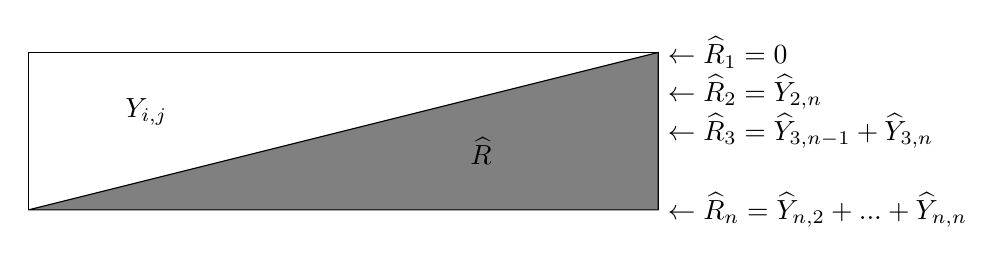
\begin{tikzpicture}
\draw (0,0) rectangle +(8,2);
\draw [fill = gray] (0,0) --(8,2) -- (8,0) -- (0,0);
\node at (1.5,1.25) {$Y_{i,j}$};
\node at (5.75,0.75) {$\widehat{R}$};
\node [right] at (8,2) {$\leftarrow\widehat{R}_1 = 0$};
\node [right] at (8,1.5) {$\leftarrow\widehat{R}_2 = \widehat{Y}_{2,n}$};
\node [right] at (8,1) {$\leftarrow\widehat{R}_3 = \widehat{Y}_{3,n-1} + \widehat{Y}_{3,n}$};
\node [right] at (8,0) {$\leftarrow\widehat{R}_n = \widehat{Y}_{n,2} + ... + \widehat{Y}_{n,n}$};
\end{tikzpicture}
\begin{align*}
\widehat{R}= \sum_{i=1}^{n} \widehat{R}_i
\end{align*}

\begin{align*}
\widehat{Y}_{2,n} &= e^{\widehat{\mu} + \widehat{\alpha}_2 + \widehat{\beta}_n} \\
\widehat{Y}_{3,n-1} &= e^{\widehat{\mu} + \widehat{\alpha}_3 + \widehat{\beta}_{n-1}} \\
\widehat{Y}_{3,n} &= e^{\widehat{\mu} + \widehat{\alpha}_3 + \widehat{\beta}_n} \\
\end{align*}

\end{itemize}

\begin{align*}
\widehat{Y}_{2,n} &= E \Bigg[ e^{\widehat{\mu} + \widehat{\alpha}_2 + \widehat{\beta}_n} \Bigg] \\
&\neq e^{E[\widehat{\mu}] + E[\widehat{\alpha}_2] + E[\widehat{\beta}_n]} \\
\end{align*}
Car $ E[g(X_1,...,X_n)]$ n'égale pas toujours égale à $g(E[X_1],...,E[X_n])$.

\subsection*{Théorème}
Soit $Y = g(X_1,...,X_n)$; une statistique fonction de la $v.a$ $X_1,...,X_n$. En développant la fonction $g(\bullet)$ en série de Taylor multidimensionnelle, et en tronquant après l'ordre 2, on trouve que
\begin{equation}
\label{eq:E[y]}
E[y] \approx g(E[X_1],...,E[X_n]) + \frac{1}{2} \sum_{i=1}^{n} \sum_{j=1}^{n} \frac{\partial^2 g(E[X_1],...,E[X_n])}{\partial X_i \partial X_j} \times \text{Cov}(X_i, X_j) 
\end{equation}
\begin{equation}
\label{eq:Var[y]}
\text{Var}(Y) \approx \sum_{i=1}^{n} \sum_{j=1}^{n} \Bigg( \frac{\partial}{\partial x_i} g(E[X_1],...,E[X_n]) \Bigg) \Bigg( \frac{\partial}{\partial x_j} g(E[X_1],...,E[X_n]) \Bigg) \times \text{Cov}(X_i, X_j)
\end{equation}

\subsubsection*{Exemple}
À partir des équations \ref{eq:E[y]} et \ref{eq:Var[y]} et en posant n = 5, on développe les équations suivantes :
\begin{align*}
\widehat{R}_3 &= \widehat{Y}_{3,4} + \widehat{Y}_{3,5} \\
&= e^{\widehat{\mu} + \widehat{\alpha}_3 + \widehat{\beta}_4} +  e^{\widehat{\mu} + \widehat{\alpha}_3 + \widehat{\beta}_5} \\
&= g(\widehat{\mu}, \widehat{\alpha}_3, \widehat{\beta}_4, \widehat{\beta}_5)
\end{align*}

On développe l'expression de l'espérance de $\widehat{R}_3$
\begin{align*}
E[\widehat{R}_3] & \cong e^{\widehat{\mu} + \widehat{\alpha}_3 + \widehat{\beta}_4} +  e^{\widehat{\mu} + \widehat{\alpha}_3 + \widehat{\beta}_5} \\
& + \frac{1}{2} \Bigg( \Big[ e^{\widehat{\mu} + \widehat{\alpha}_3 + \widehat{\beta}_4} +  e^{\widehat{\mu} + \widehat{\alpha}_3 + \widehat{\beta}_5} \Big] \text{Var}(\widehat{\mu}) \\
& + 2 \Big[ e^{\widehat{\mu} + \widehat{\alpha}_3 + \widehat{\beta}_4} +  e^{\widehat{\mu} + \widehat{\alpha}_3 + \widehat{\beta}_5} \Big] \times \text{Cov}(\widehat{\mu}, \widehat{\alpha}_3) \\
& + 2 \Big[ e^{\widehat{\mu} + \widehat{\alpha}_3 + \widehat{\beta}_4}  \Big] \times \text{Cov}(\widehat{\mu}, \widehat{\beta}_4)\\
& + 2 \Big[ e^{\widehat{\mu} + \widehat{\alpha}_3 + \widehat{\beta}_5}  \Big] \times \text{Cov}(\widehat{\mu}, \widehat{\beta}_5)\\
& + \Big[ e^{\widehat{\mu} + \widehat{\alpha}_3 + \widehat{\beta}_4} +  e^{\widehat{\mu} + \widehat{\alpha}_3 + \widehat{\beta}_5} \Big] \times \text{Cov}(\widehat{\alpha}_3, \widehat{\alpha}_3) \\
& + 2 \Big[ e^{\widehat{\mu} + \widehat{\alpha}_3 + \widehat{\beta}_4}  \Big] \times \text{Cov}(\widehat{\alpha}_3, \widehat{\beta}_4)\\
& + 2 \Big[ e^{\widehat{\mu} + \widehat{\alpha}_3 + \widehat{\beta}_5}  \Big] \times \text{Cov}(\widehat{\alpha}_3, \widehat{\beta}_5)\\
& + \Big[ e^{\widehat{\mu} + \widehat{\alpha}_3 + \widehat{\beta}_4}  \Big] \times \text{Var}(\widehat{\beta}_4)\\
& + 2 \Big[ 0 \Big] \times \text{Cov}(\widehat{\beta}_4, \widehat{\beta}_5)\\
& + 2 \Big[ e^{\widehat{\mu} + \widehat{\alpha}_3 + \widehat{\beta}_5}  \Big] \times \text{Var}(\widehat{\beta}_5) \Bigg)
\end{align*}

On développe l'expression de la variance de $\widehat{R}_3$
\begin{align*}
\text{Var}(\widehat{R}_3) & = \Bigg(  e^{\widehat{\mu} + \widehat{\alpha}_3 + \widehat{\beta}_4} +  e^{\widehat{\mu} + \widehat{\alpha}_3 + \widehat{\beta}_5}\Bigg)^2 \times \text{Var}(\widehat{\mu}) \\
& + 2 \Bigg( e^{\widehat{\mu} + \widehat{\alpha}_3 + \widehat{\beta}_4} +  e^{\widehat{\mu} + \widehat{\alpha}_3 + \widehat{\beta}_5} \Bigg)^2 \text{Cov}(\widehat{\mu}, \widehat{\alpha}_3) \\
& + 2 \Bigg( e^{\widehat{\mu} + \widehat{\alpha}_3 + \widehat{\beta}_4} +  e^{\widehat{\mu} + \widehat{\alpha}_3 + \widehat{\beta}_5} \Bigg) \Bigg( e^{\widehat{\mu} + \widehat{\alpha}_3 + \widehat{\beta}_4} \Bigg)  \times \text{Cov}(\widehat{\mu}, \widehat{\beta}_4) \\
& + 2 \Bigg( e^{\widehat{\mu} + \widehat{\alpha}_3 + \widehat{\beta}_4} +  e^{\widehat{\mu} + \widehat{\alpha}_3 + \widehat{\beta}_5} \Bigg) \Bigg( e^{\widehat{\mu} + \widehat{\alpha}_3 + \widehat{\beta}_5} \Bigg)  \times \text{Cov}(\widehat{\mu}, \widehat{\beta}_5) \\
& + \Bigg( e^{\widehat{\mu} + \widehat{\alpha}_3 + \widehat{\beta}_4} + e^{\widehat{\mu} + \widehat{\alpha}_3 + \widehat{\beta}_5}  \Bigg)^2 \times \text{Var}(\widehat{\alpha}_3)\\
& + 2 \Bigg( e^{\widehat{\mu} + \widehat{\alpha}_3 + \widehat{\beta}_4} +  e^{\widehat{\mu} + \widehat{\alpha}_3 + \widehat{\beta}_5} \Bigg) \Bigg( e^{\widehat{\mu} + \widehat{\alpha}_3 + \widehat{\beta}_4} \Bigg)  \times \text{Cov}(\widehat{\alpha}_3, \widehat{\beta}_4) \\
& + 2 \Bigg( e^{\widehat{\mu} + \widehat{\alpha}_3 + \widehat{\beta}_4} +  e^{\widehat{\mu} + \widehat{\alpha}_3 + \widehat{\beta}_5} \Bigg) \Bigg( e^{\widehat{\mu} + \widehat{\alpha}_3 + \widehat{\beta}_5} \Bigg)  \times \text{Cov}(\widehat{\alpha}_3, \widehat{\beta}_5) \\
& + \Bigg( e^{\widehat{\mu} + \widehat{\alpha}_3 + \widehat{\beta}_4}  \Bigg)^2 \times \text{Var}(\widehat{\beta}_4)\\
& + 2 \Bigg( e^{\widehat{\mu} + \widehat{\alpha}_3 + \widehat{\beta}_4} +  e^{\widehat{\mu} + \widehat{\alpha}_3 + \widehat{\beta}_5} \Bigg) \times \text{Cov}(\widehat{\beta}_4, \widehat{\beta}_5)\\
& + \Bigg( e^{\widehat{\mu} + \widehat{\alpha}_3 + \widehat{\beta}_5}  \Bigg)^2 \times \text{Var}(\widehat{\beta}_5)
\end{align*}

\subsection*{Cas de la loi Poisson}
Dans ce cas, on suppose que $Y_{i,j} \sim Poisson(\mu_{i,j})$ où $\mu_{i,j} = E[Y_{i,j}] = \text{Var}(Y_{i,j})$ et $\mu_{i,j} = e^{\mu + \alpha_i + \beta_j}$ avec $\alpha_1 = \beta_1 = 0$.
Alors, 
\begin{align*}
\phi(\Theta) &= \sum_{i, j \in \triangleleft} \text{ln} \big(f_{Y_{i,j}}(y_{i,j}) \big) \\
&= \sum_{i, j \in \triangleleft} \text{ln} \Bigg( \frac{e^{-\mu_{i,j}} \mu_{i,j}^{y_{i,j}}}{\fact{ y_{i,j}}} \Bigg) \\
&= \sum_{i, j \in \triangleleft} \Bigg( y_{i,j} \text{ln}(\mu_{i,j}) -\mu_{i,j} - \text{ln}(\fact{ y_{i,j}}) \Bigg) \\
\end{align*}

\subsection*{Log-Vraisemblance proportionnelle}
\begin{align*}
\phi(\Theta) &\simeq \sum_{i, j \in \triangleleft} \Bigg( y_{i,j} \text{ln}(\mu_{i,j}) -\mu_{i,j} \Bigg) \\
&= \sum_{i, j \in \triangleleft} \Bigg( y_{i,j} (\mu + \alpha_i + \beta_j) - e^{\mu + \alpha_i + \beta_j} \Bigg) \\
\end{align*}

En pratique, il est impossible de trouver les paramètres tels que $( \widehat{\mu}, \widehat{\alpha_2}, ..., \widehat{\alpha_n}, \widehat{\beta_1},..., \widehat{\beta_n})$ qui maximisent $\phi(\Theta)$ de manière exacte. On utilise donc l'algorithme de  \href{https://fr.wikipedia.org/wiki/Méthode_de_Newton}{Newton-Raphson}.

\begin{align*}
\Theta =
\begin{bmatrix} 
\mu \\
\alpha_2 \\
\vdots \\
\alpha_n \\
\beta_2 \\
\vdots \\
\beta_n \\
\end{bmatrix}
\end{align*}

Avec la méthode de Newton-Raphson : $\Theta^{(i+1)} = \Theta^{(i)} + I(\Theta^{(i)})^{-1}S(\Theta^{(i)})$
Rappel du cours de modèle linéaire : Dans le cas Poisson, on a trouvé que:
$$ S(\Theta) = \mathbb{X}^T \mathbb{W} \text{ ; Où } \mathbb{W} = \mathbb{Y} - \widehat{\mathbb{Y}} $$

De plus, on a
$$
I(\Theta) = \mathbb{X}^\intercal \mathbb{H} \mathbb{X}
$$


\begin{align*}
\mathbb{H} =
\begin{bmatrix} 
e^{X_1 \beta} & \cdots & 0 & \cdots & 0 \\
0  & e^{X_2 \beta} & 0 & \cdots & 0 \\
\vdots & \cdots & \ddots & \cdots & \vdots\\
0 & \cdots & 0 & e^{X_{n-1} \beta} & 0\\
0 & \cdots & 0 & \cdots & e^{X_n \beta}\\
\end{bmatrix}
\end{align*}

\subsubsection*{Remarque}
Dans les formules précédentes de $S(\Theta)$ et $I(\Theta)$; on utilise la formulation sur les GLM acquise dans le cours de modèle linéaire (ACT-2003), soit
$$
Y_{i,j} \sim \text{Poisson}(e^{\mu + \alpha_i + \beta_i}) \sim \text{Poisson}(e^{\mathbb{X} \utilde{\beta}})
$$
Où,
\begin{align*}
\utilde{\beta}=
\begin{bmatrix} 
\beta_0 \\
\beta_1 \\
\vdots \\
\beta_n \\
\end{bmatrix}
\end{align*}

\subsubsection*{Exemple}
Si n = 5, on obtient
\begin{align*}
X_{i,0} &= 1 \\
X_{i,1} &= 1\lbrace i = 2 \rbrace     & X_{i,5} &= 1\lbrace j = 2 \rbrace\\
X_{i,2} &= 1\lbrace i = 3 \rbrace     & X_{i,6} &= 1\lbrace j = 3 \rbrace\\
X_{i,3} &= 1\lbrace i = 4 \rbrace     & X_{i,7} &= 1\lbrace j = 4 \rbrace\\
X_{i,4} &= 1\lbrace i = 5 \rbrace     & X_{i,8} &= 1\lbrace j = 5 \rbrace\\
\end{align*}

\newpage
On exprime les données dans la table suivante:

\begin{center}
\begin{tabular}{|c|c|c|c|c|c|c|c|}
  \hline
   i & j & $Y_{i,j}$ & $X_{i,0}$  & $X_{i,1}$ & $X_{i,2}$ & $\ldots$ & $X_{i,8}$\\
  \hline
  1 & 1 & $\vdots$ & 1 & 1 & 0 & $\cdots$ & 0\\
  1 & 2 & $\vdots$ & 1 & 1 & 0 & $\cdots$ & 0\\
  1 & 3 & $\vdots$ & 1 & 1 & 0 & $\cdots$ & 0\\
  1 & 4 & $\vdots$ & 1 & 1 & 0 & $\cdots$ & 0\\
  1 & 5 & $\vdots$ & 1 & 1 & 0 & $\cdots$ & 1\\
  2 & 1 & $\vdots$ & 1 & 0 & 1 & $\cdots$ & 0\\
  2 & 2 & $\vdots$ & 1 & 0 & 1 & $\cdots$ & 0\\
  2 & 3 & $\vdots$ & 1 & 0 & 1 & $\cdots$ & 0\\
  2 & 4 & $\vdots$ & 1 & 0 & 1 & $\cdots$ & 0\\
  $\vdots$ & $\vdots$ & $\vdots$ & 1 & 0 & 0 & $\vdots$ & $\vdots$ \\
  4 & 1 & $\vdots$ & 1 & 0 & 0 & $\cdots$ & $\vdots$ \\
  4 & 2 & $\vdots$ & 1 & 0 & 0 & $\cdots$ & $\vdots$ \\
  5 & 1 & $\vdots$ & 1 & 0 & 0 & $\cdots$ & $\vdots$ \\
  \hline
\end{tabular}

\end{center}
\subsection*{Suite de l'exemple Excel avec n = 5}
\begin{align*}
\widehat{R} &= 0 \\
&+ \widehat{Y}_{2,5} \\
&+ \widehat{Y}_{3,4} + \widehat{Y}_{3,5} \\
&+ \widehat{Y}_{4,3} + \widehat{Y}_{4,4} + \widehat{Y}_{4,5} \\
&+ \widehat{Y}_{5,2} + \widehat{Y}_{5,3} + \widehat{Y}_{5,4} +  \widehat{Y}_{5,5}\\
\end{align*}

\newpage

On définit $\mathbb{X}^*$ comme suit

\begin{align*}
\mathbb{X}^* =
\begin{bmatrix} 
X^*_0 \\
X^*_1 \\
X^*_2 \\
X^*_3 \\
X^*_4 \\
X^*_5 \\
X^*_6 \\
X^*_7 \\
X^*_8 \\
X^*_9 \\
X^*_{10} \\
\end{bmatrix}
=
\bordermatrix { 
& \mu  &\alpha_2 &\alpha_3 &\alpha_4 & \alpha_5  & \beta_2 & \beta_3 & \beta_4 & \beta_5 \cr 
& 1 & 1 & 0 & 0 & 0 & 0 & 0 & 0 & 1 \cr 
& 1 & 0 & 1 & 0 & 0 & 0 & 0 & 1 & 0 \cr 
& 1 & 0 & 1 & 0 & 0 & 0 & 0 & 0 & 1 \cr 
& 1 & 0 & 0 & 1 & 0 & 0 & 1 & 0 & 0 \cr 
& 1 & 0 & 0 & 1 & 0 & 0 & 0 & 1 & 0 \cr 
& 1 & 0 & 0 & 1 & 0 & 0 & 0 & 0 & 1 \cr 
& 1 & 0 & 0 & 0 & 1 & 1 & 0 & 0 & 0 \cr 
& 1 & 0 & 0 & 0 & 1 & 0 & 1 & 0 & 0 \cr 
& 1 & 0 & 0 & 0 & 1 & 0 & 0 & 1 & 0 \cr 
& 1 & 0 & 0 & 0 & 1 & 0 & 0 & 0 & 1 \cr 
}
\end{align*}


\begin{align*}
\widehat{R} &= e^{X_1^*\widehat{\beta}} + e^{X_2^*\widehat{\beta}} + ... + e^{X_{10}^*\widehat{\beta}} \\
&= g(\beta_0, \beta_1, ..., \beta_{10})
\end{align*}
On obtient ainsi 
\begin{equation}
E[\widehat{R}] = g(\utilde{\widehat{\beta}}) + \frac{1}{2} \sum_{i=0}^{8} \sum_{j=0}^{8} \Bigg( \frac{\partial^2 \widehat{R}}{\partial \utilde{\beta}^2} \Bigg)_{i+1,j+1} \times I^{-1}(\utilde{\widehat{\beta}})_{i+1,j+1}
\end{equation}

Où 
\begin{align*}
\frac{\partial^2 \widehat{R}}{\partial \utilde{\widehat{\beta}}^2} &= [X^*_1]_{i+1} [X^*_1]_{j+1} \times e^{X_1 \utilde{\widehat{\beta}}} + \cdots + [X^*_{10}]_{i+1} [X^*_{10}]_{j+1} \times e^{X_{10}\utilde{\widehat{\beta}}} \\
&= (\mathbb{X}^*)^\intercal \mathbb{W}\mathbb{X}^*
\end{align*}
Où
\begin{align*}
\mathbb{W} = 
\begin{bmatrix} 
e^{X_{1}\utilde{\widehat{\beta}}} & 0 & \cdots & 0 \\
0 & e^{X_{2}\utilde{\widehat{\beta}}}  & \cdots & 0\\
\vdots & \vdots & \ddots & \vdots \\
0 & \cdots & e^{X_{9}\utilde{\widehat{\beta}}} & 0\\
0 & \cdots & 0 & e^{X_{10}\utilde{\widehat{\beta}}} \\
\end{bmatrix}
\end{align*}
Pour la variance de $\widehat{R}$, on obtient
\begin{equation}
\text{Var}(\widehat{R}) = \sum_{i=0}^{8} \sum_{j=0}^{8} \Bigg( \frac{\partial \widehat{R}}{\partial \utilde{\beta}} \Bigg)_{i+1} \times I^{-1}(\utilde{\widehat{\beta}})_{i+1,j+1} \Bigg( \frac{\partial \widehat{R}}{\partial \utilde{\beta}} \Bigg)_{j+1}
\end{equation}
Qu'on peut réécrire en vecteur de la façon suivante,
\begin{equation}
\label{eq:GLM:mat}
\text{Var}(\widehat{R}) = \Bigg( \frac{\partial \widehat{\mathbb{R}}}{\partial \utilde{\beta}} \Bigg)^\intercal I^{-1}(\utilde{\widehat{\beta}}) \Bigg( \frac{\partial \widehat{\mathbb{R}}}{\partial \utilde{\beta}} \Bigg)
\end{equation}

\subsubsection*{Note:}
\begin{align*}
\Bigg( \frac{\partial \widehat{\mathbb{R}}}{\partial \utilde{\beta}} \Bigg) &= [X^*_1] \times e^{X_1 \utilde{\widehat{\beta}}} + \cdots + [X^*_{10}] \times e^{X_{10}\utilde{\widehat{\beta}}} \\
&= (\mathbb{X}^*)^\intercal \mathbb{M}
\end{align*}
Où 
\begin{align*}
\mathbb{M} =
\begin{bmatrix} 
e^{X_1^*\utilde{\beta}} \\
e^{X_2^*\utilde{\beta}}  \\
e^{X_3^*\utilde{\beta}}  \\
e^{X_4^*\utilde{\beta}}  \\
\vdots \\
e^{X_{10}^*\utilde{\beta}} \\
\end{bmatrix}
\end{align*}

Ce qui permet de redéfinir l'équation \ref{eq:GLM:mat} de la façon suivante
\begin{align*}
\text{Var}(\widehat{R}) &= \big( (\mathbb{X}^*)^\intercal \mathbb{M} \big)^\intercal \times I^{-1}(\utilde{\widehat{\beta}}) \times \big( (\mathbb{X}^*)^\intercal \mathbb{M} \big) \\
&= \big( (\mathbb{X}^*)^\intercal \mathbb{\widehat{Y}} \big)^\intercal \times I^{-1}(\utilde{\widehat{\beta}}) \times \big( (\mathbb{X}^*)^\intercal \mathbb{\widehat{Y}} \big)
\end{align*}
Où $\mathbb{\widehat{Y}}$ correspond à la matrice des valeurs des incrémentations estimées.


\subsection*{Tests d'hypothèses avec les GLM}
$H_0$ : Un \textit{sous-modèle} de $M_1$ (noté $M_0$) est acceptable. \newline
$H_1$ : Il est nécessaire d'utiliser le modèle \textit{complet} (noté $M_1$)

Pour tester $H_0$ contre $H_1$, on obtient la statistique 
\begin{equation}
\label{eq:chisquare}
\chi_{obs}^2 = 2 \times \Big( \ell(H_1) - \ell(H_0) \Big)
\end{equation}
Et on rejette $H_0$ au niveau de confiance $100 \times (1 - \alpha) \%$ si \footnote{Où $\Xi$ corresponds au nombre de paramètres.}
\begin{equation}
\label{eq:test:chi}
\chi_{obs}^2 \geq \chi_{\alpha}^2\Big( \text{Nombre de paramètres($\Xi$) de ($M_1$) - Nombre de paramètres($\Xi$) de ($M_0$)} \Big)
\end{equation}


\subsubsection*{Exemple}
Tableau des données : \\
\begin{center}
\begin{tabular}{|c|c|c|c|c|c|}
  \hline
   i / j & 1 & 2  & 3 & 4 \\
  \hline
  1 & 100 & 48 & 23 & 10 \\
  2 & 115 & 55 & 27 &   \\
  3 & 115 & 56 & &   \\
  4 & 115 &  &  &  \\
  \hline
\end{tabular}
\end{center}
\bigskip

\begin{itemize}
\item[A)] 
\begin{align*}
E[Y_{i,j}] &= e^{\mu + \alpha_i + \beta_j} \text{; } \alpha_1 = \beta_1 = 0 \\
\widehat{\mu} &= 4.60 \\
\Xi &= 7 \\
\ell(\widehat{\beta}) & = 2249.283 \\
\end{align*} 
\begin{center}
\begin{tabular}{|c|c|c|}
  \hline
   i / j & 1 & 2\\ 
  \hline
  1 & $\phi$ & $\phi$  \\
  2 & 0.14 & -0.73    \\
  3 & 0.15 & -1.46    \\
  4 & 0.14 &  -2.30  \\
  \hline
\end{tabular}
\end{center}
\bigskip

\item[B)] 
\begin{align*}
E[Y_{i,j}] &= e^{\mu + \alpha_i + \beta \times (j-1)} \text{; } \alpha_1 = 0 \\
\widehat{\mu} &= 4.60 \\
\widehat{\beta} &= -0.74 \\
\Xi &= 5 \\
\ell(\widehat{\beta}) & = 2249.283 \\
\widehat{\alpha}_2 &= 0.15 \\
\widehat{\alpha}_3 &= 0.15 \\
\widehat{\alpha}_4 &= 0.14 \\
\end{align*} 
\subsubsection*{Test}
À l'aide de l'équation \ref{eq:chisquare} on effectue le test d'hypothèse suivant \newline
$H_0$ : Linear developpment $\beta_j = \beta \times (j-1)$ \newline
$H_1$ :  No linear development
\begin{align*}
\chi_{obs}^2 &= 2 \times \Big( 2249.283 - 2248.234 \Big) \\
&= 0.098087 \\
\chi_{0.05}^2(7 - 5) &= 5.99 \\
\end{align*}
Pour rejeter $H_0$, on doit satisfaire l'équation \ref{eq:test:chi},
\begin{align*}
\chi_{obs}^2 &\geq \chi_{\alpha}^2\Big( \Xi (M_1) - \Xi (M_0) \Big) \\
0.098087 &\overset{?}{\geq} 5.99 \\
\end{align*}
On ne peut pas rejeter $H_0$.
\bigskip

\item[C)]
\begin{align*}
E[Y_{i,j}] &= e^{\mu + \alpha\times(i-1) + \beta \times (j-1)} \\
\widehat{\mu} &= 4.64 \\
\widehat{\alpha} &= 0.05 \\
\widehat{\beta} &= -0.73 \\
\Xi &= 3 \\
\ell(\widehat{\beta}, \widehat{\alpha}, \widehat{\mu}) & = 2248.644 \\
\end{align*} 
\subsubsection*{Test}
$H_0$ : Linear trend and developpment ( $e^{\mu + \alpha(i-1) + \beta \times (j-1)}$) \newline
$H_1$ : $H_0$ is false ( $e^{\mu + \alpha_i + \beta_j}$)
\begin{align*}
\chi_{obs}^2 &= 2 \times \Big( 2249.283 - 2248.664 \Big) \\
&= 1.024 \\
\chi_{0.05}^2(7 - 3) &= 9.488 \\
\end{align*}

Pour rejeter $H_0$, on doit satisfaire l'équation \ref{eq:test:chi},
\begin{align*}
\chi_{obs}^2 &\geq \chi_{\alpha}^2\Big( \Xi (M_1) - \Xi (M_0) \Big) \\
1.024 &\overset{?}{\geq} 9.488\\
\end{align*}
On ne peut pas rejeter $H_0$.
\bigskip

\subsubsection*{Alternative au test d'hypothèse}
$H_0$ : Linear trend and developpment ( $e^{\mu + \alpha(i-1) + \beta \times (j-1)}$) \newline
$H_1$ : $H_0$ is false ( $e^{\mu + \alpha_i + \beta \times (j-i)}$)

\bigskip
\item[D)]
On sait qu'il y a eu une nouvelle loi sur le règlement des sinistres à partir de l'année de calendrier 3. $I_{i,j}$ = indicateur de nouvelle loi à i, j.

\begin{center}
\begin{tabular}{|c|c|c|c|c|}
  \hline
   i / j & 1 & 2 & 3 & 4\\ 
  \hline
  1 & 0 & 0 & 1 & 1  \\
  2 & 0 & 1 & 1 &  \\
  3 & 1 & 1 & &   \\
  4 & 1 &  &  &  \\
  \hline
\end{tabular}
\end{center}
\bigskip
\begin{align*}
E[Y_{i,j}] &= e^{\mu + \alpha\times(i-1) + \beta \times (j-1)} + \alpha I_{i,j} \\
\end{align*}
Pour tester si la nouvelle loi a un impact sur le développement, on utilise le $H_0$ suivant
\begin{align*}
H_0 &= e^{\mu + \alpha\times(i-1) + \beta \times (j-1)} \\
\widehat{\mu} &= 4.64 \\
\widehat{\alpha} &= 0.05 \\
\widehat{\beta} &= -0.73 \\
\Xi &= 3 \\
\ell(\widehat{\beta}, \widehat{\alpha}, \widehat{\mu}, \widehat{\alpha}) & = 2248.644 \\
\end{align*}
et le $H_1$ suivant
\begin{align*}
H_1 &= e^{\mu + \alpha\times(i-1) + \beta \times (j-1) + \alpha I_{i,j}} \\
\widehat{\mu} &= 4.64 \\
\widehat{\alpha} &= 0.05 \\
\widehat{\beta} &= -0.73 \\
\widehat{\alpha} &= -001644 \\
\Xi &= 4 \\
\ell(\widehat{\beta}, \widehat{\alpha}, \widehat{\mu}, \widehat{\alpha}) & = 2248.649 \\
\end{align*}
\subsubsection*{Test}
En utilisant les hypothèses $H_0$ et $H_1$ précédentes,
\begin{align*}
\chi_{obs}^2 &= 2 \times \Big( 2248.649-2248.644 \Big) \\
&= 0.009305 \\
\chi_{0.05}^2(4 - 3) &= 3.84 \\
\end{align*}
Pour rejeter $H_0$, on doit satisfaire l'équation \ref{eq:test:chi},
\begin{align*}
\chi_{obs}^2 &\geq \chi_{\alpha}^2\Big( \Xi (M_1) - \Xi (M_0) \Big) \\
0.009305 &\overset{?}{\geq} 3.84\\
\end{align*}
On ne peut pas rejeter $H_0$.
\bigskip
\end{itemize}

\section{Méthode de réserve IARD basée sur la théorie de la crédibilité}

\subsubsection*{Rappel sur C-L }
\begin{enumerate}
\item Le modèle est  bon pour les vieilles AA. Il y a beaucoup de données disponibles, autrement dit, d'expérience individuelle est \textit{crédible}.
\item Par contre, il est moins bon pour les AA récentes. Il y a moins de données, autrement dit, l'expérience individuelle est moins volumineuse et donc moins crédible 
\end{enumerate}
L'idée : Accorder plus de crédibilité à C-L si AA vieille, donc on possède beaucoup de données, et de donner plus de crédibilité à B-F si AA récente.

\subsubsection*{Rappel}
\begin{align*}
\widehat{R}_i^{C-L} &= \widehat{C}_{i,n}^{C-L} - C_{i, n-i+1} \\
&= C_{i,n-i+1} \times \Big(\prod_{j=n-i-1}^{n-1} LDF_j \Big) - C_{i,n-i+1}\\
&= C_{i,n-i+1} \times \Big(\prod_{j=n-i-1}^{n-1} LDF_j - 1 \Big) \\
\end{align*}
\begin{align*}
\widehat{R}_i^{B-F} &= \widehat{C}_{i,n}^{B-F} - C_{i, n-i+1} \\
&= PA_i \times LR_i  - C_{i, n-i+1}\\
&= U_i - \frac{U_i}{\prod_{j=n-i-1}^{n-1} LDF_j}\\
&= U_i \Bigg( 1 - \frac{1}{\prod_{j=n-i-1}^{n-1} LDF_j} \Bigg) \text{; posons } \beta_{n-i+1} = \frac{1}{\prod_{j=n-i-1}^{n-1} LDF_j}\\
&= U_i \Bigg( 1 - \beta_{n-i+1} \Bigg) \\
\end{align*}
L'idée est de combiner $\widehat{R}_i^{C-L}$  et $\widehat{R}_i^{B-F}$.

\begin{align*}
\widehat{R}_i^{Cred} &= C_i \widehat{R}_i^{C-L} + (1 - C_i) \widehat{R}_i^{B-F} \\
&= C_i \times C_{i, n-i+1} \Bigg( \prod_{j=n-i-1}^{n-1} LDF_j - 1 \Bigg) + (1 - C_i) U_i (1 - \beta_{n-i+1}) \\
&= C_i \times C_{i, n-i+1} \Bigg( \prod_{j=n-i-1}^{n-1} LDF_j - 1 \Bigg) + (1 - C_i) U_i (1 - \beta_{n-i+1}) \\
&=C_i \times \widehat{C}_{i, n}^{C-L} - C_i C_{i, n-i+1}  + (1 - C_i) U_i - (1 - C_i)U_i (1 - \beta_{n-i+1}) \\
&= [C_i \times \widehat{C}_{i, n}^{C-L} + (1 - C_i) U_i] - \beta_{n-i+1}\Bigg[ \frac{C_i C_{i, n-i+1}}{\beta_{n-i+1} } + (1 - C_i)U_i\Bigg] \\
\end{align*}
On développe $\beta_{n-i+1}$ afin de réduire l'expression précédante,
\begin{align*}
\beta_{n-i+1} &= \frac{1}{\prod_{j=n-i-1}^{n-1} LDF_j} \\
\frac{1}{\beta_{n-i+1}} &= \prod_{j=n-i-1}^{n-1} LDF_j \\
\frac{C_{i, n-i+1}}{\beta_{n-i+1}} &= C_{i, n-i+1} \prod_{j=n-i-1}^{n-1} LDF_j \\
\frac{C_i C_{i, n-i+1}}{\beta_{n-i+1}} &= C_i C_{i, n-i+1} \prod_{j=n-i-1}^{n-1} LDF_j \\
\frac{C_i C_{i, n-i+1}}{\beta_{n-i+1}} &= C_i \widehat{C}_{i, n}^{C-L} \\
\end{align*}
À partir de cette \textit{identité} et de l'expression suivante, on obtient le résultat suivant
\begin{align*}
\widehat{R}_i^{Cred} &= [C_i \times \widehat{C}_{i, n}^{C-L} + (1 - C_i) U_i] - \beta_{n-i+1} \Bigg[ C_i C_{i, n}^{C-L}  + (1 - C_i)U_i \Bigg] \\
&= [C_i \times \widehat{C}_{i, n}^{C-L} + (1 - C_i) U_i] ( 1 - \beta_{n-i+1}) \\
\end{align*}

Que l'on peut réécrire de la façon suivante
\begin{equation}
\widehat{R}_i^{Cred} = \Bigg[C_{i, n - i + 1} + \Bigg(1 - \frac{1}{\prod_{j = n - i + 1}^{n- 1} \widehat{LDF}_j} \Bigg) PA_i \times LR_i \Bigg] \Bigg(1 - \frac{1}{\prod_{j = n - i + 1}^{n- 1} \widehat{LDF}_j} \Bigg) \\
\end{equation}


Au début des années 1980, Benktander et Hovinen ont trouvé le raisonnement suivant :
\begin{itemize}
\item[i)] $U_i (1 - \beta_{n-i+1}) = R_i^{B-F}$
\item[ii)] $\widehat{R}_i^{B-F} = U_i - C_{i,n-i+1} \Rightarrow \widehat{R}_i^{B-F} = U_i^{B-H} - \widehat{C}_{i,n}\beta_{n-i+1}$
\end{itemize}
À partir de i) $\rightarrow$ ii), on obtient le développement suivant
\begin{align*}
\widehat{C}_{i, n}^{B-F} ( 1 - \beta_{n-i+1} )  &= U_i ^{B-H} - \beta_{n-i+1} \widehat{C}_{i, n}^{C-L} \\
U_i ^{B-H} &= \beta_{n-i+1} \widehat{C}_{i, n}^{C-L} + ( 1 - \beta_{n-i+1} )\widehat{C}_{i, n}^{B-F}  \\
\widehat{C}_{i,n}^{B-H} &= \beta_{n-i+1} \widehat{C}_{i, n}^{C-L} + ( 1 - \beta_{n-i+1} )\widehat{C}_{i, n}^{B-F}  \\
\end{align*}
Où $\beta_{n-i+1}$ correspond à $C_i$ et $( 1 - \beta_{n-i+1} )$ correspond à $ 1 - C_i$.
\newline

En conclusion, pour que l'hypothèse de Benktander - Hoviden soit respectée, autrement dit, à la coïncidence  des diagonales du triangle,  il faut que 
\begin{equation}
C_i = \beta_{n-i+1} = \frac{1}{\prod_{j=n-i+1}^{n-1}} = \text{ La proportion de ce qui a été fait}
\end{equation}

\subsubsection*{Remarque}
En pratique, cette méthode est appelée Bornhuetter - Ferguson itérée. \newline
En répétant  m fois ce raisonnement d'itération, on trouve :
\begin{align*}
 \widehat{C}_{i,n}^{B-H} =
     	\left\{
     	\begin{array}{rl}
     	C_{i,n-i+1} + ( 1 - \beta_{n-i+1} )\widehat{C}_{i, n}^{B-H (m-1)} &, \text{si } m \geq 1 \\
		  C_{i,n-i+1} + ( 1 - \beta_{n-i+1} )U_i &, \text{si } m = 0
     	\end{array}
     	\right.
\end{align*}
Où $U_i = PA_i \times LR_i$
\begin{align*}
\widehat{R}_i^{B-H(m)} = \widehat{C}_{i, n}^{B-H (m)} - C_{i,n-i+1}
\end{align*}
\section{Actualisation des réserves IARD}
Il faut se rappeler qu'on actualise selon l'année de calendrier (Calendar Year (CY))

\begin{center}
\begin{tabular}{|c|c|c|c|c|c|c|c|c|c|}
  \hline
   i & 0 & 12 & 24 & 36 & 48 & 72 & 84 & 0  \\
  \hline
  2005 & & & & & & & & \\
  2006 & & & & & & & & \\
  2007 & & & & & & & & \\
  2008 & & & & & & & & 2015 \\
  2009 & & & & & & & 2015 & 2016 \\
  2010 & & & & & & 2015 & 2016 & 2017 \\
  2011 & & & & & 2015 & 2016 & 2017 & 2018 \\
  2012 & & & & 2015 & 2016 & 2017 & 2018 & 2019  \\
  2013 & & & 2015 & 2016 & 2017 & 2018 & 2019 & 2020  \\
  2014 & & 2015 & 2016 & 2017 & 2018 & 2019 & 2020 & 2021  \\
  \hline
\end{tabular}
\end{center}

\subsubsection*{Étapes}
\begin{itemize}
\item[1)] Développer le triangle avec l'une des méthodes vues en classe : C-L, B-F, Mack, GLM ou B-H.
\item[2)] Calculer les sinistres incrémentaux $Y_{i,j}$ dans la partie inférieure du triangle
\item[3)] Sommer les $Y_{i,j}$ de l'étape 2 par année de calendrier (CY)
\item[4)] Actualiser par CY

\begin{center}
\begin{tabular}{|c|c|c|c|c|c|}
  \hline
   CY & $\sum Y_i$ & Duration & Annual yield curve rate & Actualized figure \\
  \hline
  2015 & $CF_{15}$ & 0.5 & 1 \% & $CF_{15} (1 + 0.01)^{-0.5}$ \\
  2016 & $CF_{16}$ & 1.5 & 2 \% &  $CF_{16} (1 + 0.02)^{-1.5}$\\
  $\vdots$ & $\vdots$ & $\vdots$ & $\vdots$ & $\vdots$  \\
  2021 & $CF_{21}$ & 6.5 & 5 \% & $CF_{21} (1 + 0.05)^{-6.5}$  \\
  \hline
\end{tabular}
\end{center}
\bigskip
$ \widehat{R} = \sum \text{Actualized figure}$ 
\\

\textbf{Notes:} Pour simplifier les calculs, on suppose une distribution uniforme [0, 1] des montants de la réserve et on utilise le point milieu pour l'actualisation.
\end{itemize}







%%%%%%%%%%%%%%%%%%%%%%%%%%%%%%%%%%%%%%%%%% Annexe #################################


\appendix
\input{tex/ann_res_intra}

\chapter{Résumé examen final}

\subsection*{But et notation} 

\begin{itemize}
\item Évaluation des réserves: Rôle de l'actuaire \textbf{corporatif}
\item Réserve IARD: Montant nécessaire pour payer les \textbf{sinistres déjà survenus à la date d'évaluation} (Sinistres dont le développement n'est pas complet)
\item Les réserves doivent être signées par un \textbf{actuaire désigné}
\item Les réserves \textbf{doivent} être évaluées au 31 décembre, mais plusieurs compagnies les évaluent au \textbf{trimestre} ou au \textbf{mois}
\end{itemize}

Il est important de bien évaluer les réserves, car

\textbf{Si les réserves sont surévaluées }:
\begin{itemize}
  \item Dépenses $\nearrow$
  \item Profits $\searrow$
  \item Impôts à payer $\searrow$
  \item Surplus de l'assureur $\searrow$
  \item Valeur de la compagnie (prix de l'action) $\searrow$
\end{itemize}


\textbf{Si les réserves sont sous-évaluées}
\begin{itemize}
  \item Surévalue la santé financière de la compagnie
  \item Expose l'assuré à ne pas être payé en cas de réclamation
  \item Expose l'assureur à la ruine
\end{itemize}


\subsection*{Définitions}

\textbf{Dossier de sinistre}:
\begin{itemize}
  \item Un dossier est ouvert à chaque fois qu'un assuré fait une réclamation.
  \item Ce dossier contient toutes les informations relatives à la réclamation (date d'accident, date de réclamation, montants et moments de chaque paiement, information qualitative).
\end{itemize}

\textbf{Case Reserves}:
\begin{itemize}
  \item Une \textit{Case Reserve} est la meilleure estimation d'un montant de sinistre avant même qu'un paiement soit fait (\textbf{expert en sinistre} ou \textbf{modèle prédictif}).
  \item Les \textit{Case Reserves} sont la somme des Case Reserves individuelles.
\end{itemize}

\textbf{Gross IBNR (ou Bulk Reserve)}
\begin{itemize}
  \item IBNR = Incurred but not Reported
  \item Contiens les provisions pour:
  \begin{itemize}
    \item Développement futur des sinistres
    \item Sinistres fermés pouvant rouvrir
    \item Sinistres encourus, mais non rapportés (Pure IBNR)
    \item Sinistres rapportés, mais non codés dans le système informatique
  \end{itemize}
\end{itemize}
 
\textbf{Réserve totale}:
$$\text{Réserve totale} = \text{Case Reserves} + \text{Gross IBNR}$$

\textbf{Développement}:
\begin{itemize}
\item Changement temporel de la somme des paiements effectués sur tous les dossiers de sinistre (Prestations payées durant une période)
\end{itemize}
  
\textbf{Paid Age-to-Age}
\begin{itemize}
\item Développement entre deux dates données (on suit généralement après chaque année ou mois d'âge successifs)
\end{itemize}
 
\textbf{Age-to-ultimate Development}
\begin{itemize}
\item Développement des sinistres ayant atteint un certain âge jusqu'à l'ultime.
\end{itemize}

\textbf{Paid Loss Development Factor ($\text{PLDF}_{j-1,j}$)}

$$\text{PLDF}_{j-1,j} = \frac{\text{Somme des paiements faits par l'assureur sur tous les dossiers de sinistres à t=j}}{\text{Somme des paiements faits par l'assureur sur tous les dossiers de sinistres à t=j-1}}$$

\textbf{Sinistres en suspend ($SS$)}
\begin{itemize}
  \item Somme des \textit{Case Reserves} qui ne sont pas encore fermées à une date donnée.
 \end{itemize}
\textbf{Sinistres payés ($SP$)}
\begin{itemize}
  \item Somme des indemnités versées aux réclamants (\textbf{inclus les frais de règlement})
 \end{itemize} 
\textbf{Sinistres encourus ($SE$)}
\begin{itemize}
  \item Somme des montants engendrés par un sinistre (Passé + Futur)
\end{itemize}
$$SE = SP + SS$$

\textbf{Incurred Loss Development Factor ($\text{ILDF}_{j-1,j}$)}

$$\text{ILDF}_{j-1,j}=\frac{\sum SE@j}{\sum SE@j-1}=\frac{C_j}{C_{j-1}}=\frac{\text{Encouru cumulatif @ t=j}}{\text{Encouru cumulatif @ t=j-1}}$$

\textbf{Notation en triangles cumulatifs}

Il est commode de noter $C_{i,j}$, le total des sinistres survenus dans l'année i développés pendant j années de la façon suivante:

\begin{tabular}{|c|c|c|c|c|c|}
  \hline
   i/j & Age 1 & Age 2 & Age 3 & Age 4 & Age 5 \\
  \hline
1 & $C_{1,1}$ & $C_{1,2}$ & \color{red} $C_{1,3}$ & $C_{1,4}$ & $C_{1,5}$ \\
2 & $C_{2,1}$ & \color{red} $C_{2,2}$ & $C_{2,3}$ & $C_{2,4}$ & \\
3 & \color{red} $C_{3,1}$ & $C_{3,2}$ & $C_{3,3}$ &  & \\
4 & $C_{4,1}$ & $C_{4,2}$ &  &  & \\
5 & $C_{5,1}$ &  &  &  & \\
  \hline
\end{tabular}\\


$\Rightarrow$ \color{red} Année de calendrier 3 \color{black}

\subsection*{Méthode de Chain-Ladder}

\subsubsection*{Notions mathématiques}

Pour la méthode de Chain-Ladder, on assume tout simplement que $LDF_j$, le taux de développement pour l'année j est le même pour toutes les années de sinistres. On a donc
$$C_{i,j+1} = C_{i,j} \times LDF_j$$

Avec
$$\widehat{LDF}_j = \frac{\sum_{i=1}^{n-j} C_{i,j+1}}{\sum_{i=1}^{n-j} C_{i,j}}, \forall j=1,...,n-1$$

Pour le calcul de la réserve IBNR, on s'intéresse à la différence entre les coûts à l'ultime, soit les coûts totaux lorsque les sinistres seront pleinement développés, et les prestations qui ont été payé jusqu'à la date d'évaluation. Il est donc crucial de bien calcul $C_{i,n}$. Pour Chain-Ladder, on a
$$\widehat{C}_{i,n} = (\widehat{LDF}_{n+1-i}\times...\times\widehat{LDF}_{n-1})\times C_{i,n+1-i}$$

Et la réserve pour l'année i est
$$\widehat{R}_i=\widehat{C}_{i,n}-C_{i,n+1-i},\forall i=2,...,n$$
Et la réserve totale est
$$\widehat{R}=\sum_{i=2}^{n} \widehat{R}_i$$

\subsubsection*{Remarques}

\begin{itemize}
\item Cette méthode suppose que les années d'accident sont indépendantes entre elles.
\item On assume aussi implicitement que l'âge des sinistres est la seule variable explicative du développement des sinistres.
\item On fait l'hypothèse simplificatrice que $LDF_{i,j}=LDF_j$. Ceci n'est pas nécessairement vrai, car plusieurs facteurs peuvent venir influencer la vitesse de développement de l'année i:
	\begin{itemize}
	\item Changements internes dans les procédures de la compagnie
	\item Changement de loi
	\item ...
	\end{itemize}
\item Avec Chain-Ladder, la réserve de l'année d'accident la plus récente est sujette à une forte incertitude, car elle dépend seulement des paiements effectués dans l'année de calendrier la plus récente.
\end{itemize}


\subsection*{Méthode de Bornhuetter-Ferguson}

\subsubsection*{Notions mathématiques}

La méthode de B-F se fait en trois grandes étapes

\subsubsection*{ Étape 1: Estimation des sinistres ultimes}

On assume que le \textbf{taux de sinistre} (Loss Ratio) est connu pour chaque année d'accident. Ainsi, soit $LR_i$ le taux de sinistre de l'année i et $PA_i$ les primes acquises pour l'année d'accident i, on a
$$\boxed{\widehat{C}_{i,n}^{(B-F)}=\widehat{LR_i} \times PA_i}$$

\subsubsection*{ Étape 2: Calcul des facteurs de développement }

Le calcul des facteurs de développement est exactement le même que pour Chain-Ladder, c'est à dire
$$\widehat{LDF}_j=\frac{\sum_{i=1}^{n-j} C_{i,j+1}}{\sum_{i=1}^{n-j} C_{i,j}}$$

\subsubsection*{ Étape 3: Calcul de la réserve }

Pour B-F, on a 

$$\boxed{\widehat{R}_i^{(B-F)}=\widehat{C}_{i,n}^{(B-F)}\times \left(1 - \frac{1}{\prod_{j=n+1-i}^{n-1} \widehat{LDF}_j} \right)}$$

\subsubsection*{  Remarques }

\begin{enumerate}
\item L'avantage de cette méthode est qu'elle permet une meilleure stabilité des réserves des années de survenance récentes.
\item L'inconvénient majeur de cette méthode est qu'elle requiert l'utilisation de données externes ($LR_i$, $PA_i$) qui introduisent de la subjectivité.
\item Dans cette méthode, c'est comme si on assumait que l'âge n'affecte pas le développement du sinistre
\end{enumerate}

$$\widehat{C}_{i,n}^{(B-F)}=PA_i \times LR_i = a_i \Rightarrow \text{ordonnée à l'origine}$$
$$\begin{aligned}
\widehat{C}_{i,n}^{(C-L)}&=C_{i,n+1-i} \times \left(\prod_{j=n+1-i}^{n-1} LDF_j \right) \\
                    &= C_{i,n+1-i} \times B_i \Rightarrow \text{Pente}
\end{aligned}$$

Il serait donc intéressant de mélanger C-L et B-F afin d'obtenir une régression linéaire avec pente et ordonnée à l'origine.

\subsection*{Méthode de Mack}

Essentiellement, la méthode de Mack est simplement la méthode de Chain-Ladder, mais avec un cadre statistique plus solide qui permet une estimation de la variance des réserves qui peut être très utile afin d'avoir une meilleure idée du risque auquel s'expose la compagnie.

\subsubsection*{ Hypothèses du modèle de Mack}

\begin{enumerate}
\item $\{C_{1,1},...,C_{1,n} \}\perp\!\!\!\perp \{C_{2,1},...,C_{2,n} \} \perp\!\!\!\perp...\perp\!\!\!\perp \{C_{n,1},...,C_{n,n} \}$
\item $ E(C_{i,k+1} | C_{i,1},...,C_{i,k})=LDF_k$
\item $Var(C_{i,k+1} | C_{i,1},...,C_{i,k}) = \sigma_k^2 \times C_{i,k}$
\end{enumerate}


\subsubsection*{ Estimation des LDF}

Notons tout d'abord $H_i$ les données historiques pour l'année d'accident i et $D$ le triangle de données complet. Comme pour le modèle Chain-Ladder, on a
$$\widehat{LDF}_j=\frac{\sum_{i=1}^{n-j} C_{i,j+1}}{\sum_{i=1}^{n-j} C_{i,j}}$$

De plus, le cadre théorique du modèle de Mack nous permet de prouver que:

$$E(C_{i,j}|D)=C_{i,n+1-i} \times LDF_{n+1-i}\times...\times LDF_{j-1}$$

On a aussi, avec $D_k$, le triangle tronqué à l'âge k, 
$$E(C_{i,k+1}|D_k) \overset{H2}{=} C_{i,k} \times LDF_k$$
et 
$$E(\widehat{LDF}_k|D_k)= \frac{\sum_{i=1}^{n-k} C_{i,k}LDF_k}{\sum_{i=1}^{n-k} C_{i,k}}=LDF_k$$

Un autre résultat important que l'on peut prouver par la méthode de Mack est que
$$\text{Cov}(\widehat{LDF}_k,\widehat{LDF}_j)=0$$

et
$$E(\widehat{R}_i)=R_i$$

\subsubsection*{ Estimation des $\sigma_j^2$}

L'estimateur non-biaisé de $\sigma^2$ est
$$\boxed{\widehat{\sigma}_j^2 = \frac{1}{n-j-1}\sum_{i=1}^{n-j}C_{i,j} \times \left(\frac{C_{i,j+1}}{C_{i,j}}-\widehat{LDF}_j \right)^2}$$
Qui correspond à l'équation \ref{eq:est:sigm}.

De plus, comme on peut le voir, le calcul de $\widehat{\sigma}^2$ est problématique pour $j=n-1$. On utilise donc l'approximation suivante:
$$\boxed{\widehat{\sigma}_{n-1}^2=min \left(\frac{\widehat{\sigma}_{n-2}^4}{\widehat{\sigma}_{n-3}^2},min \left(\widehat{\sigma}_{n-3}^2,\widehat{\sigma}_{n-2}^2 \right) \right)}$$

\subsubsection*{Estimation de l'erreur quadratique moyenne}

Tout d'abord, puisque $\widehat{R}_i$ est un estimateur non biaisé de $R$, on a $Var(\widehat{R}_i)=MSE(\widehat{R}_i)$

$$\boxed{\begin{aligned}
MSE(\widehat{R}_i) &= E\left((\widehat{R}_i-R_i)^2 | D \right) \\
MSE(\widehat{R}_i) &= \widehat{C}_{i,n}^2 \times \sum_{k=n-i+1}^{n-1} \frac{\widehat{\sigma}_k^2}{\widehat{LDF}_k^2} \times \left(\frac{1}{\widehat{C}_{i,k}}+ \frac{1}{\sum_{j=1}^{n-k} C_{j,k}} \right)
\end{aligned}}$$

\subsubsection*{ Intervalles de confiance}

En ayant maintenant estimé l'erreur quadratique moyenne des réserves calculées, il est possible de poser des hypothèses quant à la loi suivie par la réserve afin de construire une intervalle de confiance.

\subsubsection*{ Hypothèse de normalité}

Puisqu'on assume ici
$$\widehat{R}_i \sim N(E[\widehat{R}_i], \widehat{MSE}(\widehat{R}_i))$$
Ce qui impose
$$\boxed{I.C.^N(\widehat{R}_i)=\left[\widehat{R}_i - Z_{\frac{\alpha}{2}} \times \sqrt{\widehat{MSE}(\widehat{R}_i)}, \widehat{R}_i + Z_{\frac{\alpha}{2}} \times \sqrt{\widehat{MSE}(\widehat{R}_i)} \right]}$$

\subsubsection*{ Hypothèse de log-normalité}

On suppose ici
$$R_i \sim LN(\mu_i, \sigma_i^2)$$
Avec
$$\begin{aligned}
E[R_i] &= \widehat{R}_i = e^{\mu_i + \frac{\sigma^2}{2}} \\
MSE(R_i) &= E(R_i)^2 \times \left(e^{\sigma_i^2}-1 \right) \\ \\
\Leftrightarrow \mu_i &= ln(\widehat{R}_i)-\frac{\sigma_i^2}{2} \\
\Leftrightarrow \sigma_i^2 &= ln \left(1 + \left(\frac{\sqrt{\widehat{MSE}(\widehat{R}_i)}}{\widehat{R}_i}\right)^2 \right)
\end{aligned}$$

Ce qui impose
$$\boxed{I.C.^{LN}(\widehat{R}_i) = \left[e^{\mu_i - Z_{\frac{\alpha}{2}}\sigma_i}, e^{\mu_i + Z_{\frac{\alpha}{2}}\sigma_i} \right]}$$

\subsubsection*{ Variabilité de la réserve totale}

On a tout simplement 
$$\begin{aligned}
MSE(\widehat R) &= E\left[(\widehat{R}-R)^2|D \right] \\
   &= E\left(\left(\sum_{i=2}^n \widehat R_i - \sum_{i=2}^n R_i\right)^2|D \right)
\end{aligned}$$

$$\boxed{\widehat{MSE}(\widehat{R}) = \sum_{i=2}^n \left( \widehat{MSE}(\widehat{R}_i) + \widehat{C}_{i,n} \times \left(\sum_{j=i+1}^n \widehat{C}_{j,n} \right) \times \sum_{k=n-i+1}^{n-1} \frac{\frac{2\widehat{\sigma}_k^2}{\widehat{LDF}_k^2}}{\sum_{j=1}^{n-k} C_{j,k}} \right) }$$

\subsection*{ Méthode GLM}

\begin{itemize}
\item La méthode GLM ne se limite pas à la loi normale. En effet, on peut utiliser n'importe quelle loi de la famille exponentielle. (Normale, Log-Normale, Binomiale, Poisson, Gamma, Exponentielle, Inverse Gaussienne,...)
\item Permets d'incorporer au modèle des variables explicatives autres que l'âge et l'année d'accident. (Changement de VP, Changement de loi, catastrophe naturelle)
\item Permets de faire des réserves granulaires au lieu d'agréger les données par âge et année d'accident.
\end{itemize}

\subsubsection*{Remarques}
\begin{enumerate}
\item Avec les GLM, on utilise le triangle des sinistres incrémentaux ($Y_{i,j}$) et non cumulatifs ($C_{i,j}$).
\item En pratique, on utilise une loi de la famille exponentielle selon la variance observée dans les $Y_{i,j}$.
\end{enumerate}

%% Voir document goulet pour bien faire le tableau 
\begin{tabular}{|c|c|c|}
  \hline
   Loi & Fonction de variance & Utilisation en réserves  \\
  \hline
  Normale & $\sigma^2 \neq f(u)$ & Très rare, car la variance diminue avec l'âge j \\
  Poisson & $\mu$ & Souvent \\
  Gamma & var $ = f(\mu^2)$ & Moins souvent \\
  Inverse Gaussienne & var $ = f(\mu^3)$ & Très rare  \\
  \hline
\end{tabular}\\
\subsubsection*{Le modèle de base}

Si on ne se sent pas exotique, on peut passer un modèle GLM sans variables explicatives autres que l'âge et l'année d'accident. Dans ce cas, on a donc
$$\begin{aligned}
\alpha_1 &= \beta_1 = 0 \\
E[Y_{i,j}] &= \mu_{i,j} = e^{\mu + \alpha_i + \beta_j} 
\end{aligned}$$

Où on obtient ici $\tilde{\beta}=[\mu, \alpha_2,...,\alpha_n,\beta_2,...,\beta_n]$ par maximum de vraisemblance.

\subsubsection*{Un modèle plus élaboré}

Si on se sent aventurier, on peut ajouter d'autres variables explicatives à notre modèle de calcul des réserves. On pourrait par exemple ajouter la variable indicatrice d'un changement de VP $X_{i,j}$ et on obtiendrait ainsi:
$$E[Y_{i,j}]=\mu_{i,j} = e^{\mu + \alpha_i + \beta_j + \gamma X_{i,j}}$$

\subsubsection*{Théorème de Taylor multidimensionnel (nice...)}

Soit $Y=g(X_1,X_2,...,X_n)$ une fonction statistique des variables aléatoires ($X_1,...,X_n$), on a 

$$\boxed{E[Y] \approx g(E[X_1],...,E[X_n])+\frac{1}{2}\sum_{i=1}^n \sum_{j=1}^n \frac{\partial^2 g(E[X_1],..,E[X_n])}{\partial x_i \partial x_j}\text{Cov}(X_i,X_j)}$$
et
$$\boxed{Var(Y) \approx \sum_{i=1}^n \sum_{j=1}^n \left(\frac{\partial}{\partial x_i}\ g(E[X_1],...,E[X_n]) \right) \left(\frac{\partial}{\partial x_j}\ g(E[X_1],...,E[X_n]) \right) \text{Cov}(X_i, X_j)}$$

Malheureusement, puisque $Y$ peut facilement être une quantité souvent utilisée telle $\widehat{R}_i$, il faut le sentir.

\subsubsection*{Estimation des coefficients}

Tel que vu en ACT-2003, la meilleure façon d'estimer les coefficients nécessaires au calcul des réserves IARD est le maximum de vraisemblance. Dans le cas Poisson, on aurait donc

$$\begin{aligned}
\mu_{i,j} &= e^{\mu + \alpha_i + \beta_j} \\
l(\Theta) &= \sum_{(i,j) \in \rhd} ln\left(\frac{e^{-\mu_{i,j}}(\mu_{i,j})^{y_{i,j}}}{(y_{i,j})!} \right) \\
 &= \sum_{(i,j) \in \rhd} \left(y_{i,j} \ln(\mu_{i,j}) - \mu_{i,j} - \ln(y_{i,j}!) \right) \\
 &\propto \sum_{(i,j) \in \rhd} \left(y_{i,j}\ln(\mu_{i,j}) - \mu_{i,j} \right)
\end{aligned}$$

On utilise le log-vraisemblance proportionnelle pour éviter les problèmes numériques que pourraient poser le calcul de $2000!$ par exemple. 
Maintenant que la fonction à optimiser est posée, il ne reste plus qu'à la maximiser par la méthode de Newton-Raphson. On a donc

\[
\Theta = 
\begin{bmatrix}
\mu \\
\alpha_2 \\
... \\
\alpha_n \\
\beta_2 \\
... \\
\beta_n
\end{bmatrix}
\]

$$\boxed{\Theta^{(i+1)}=\Theta^{(i)}+I(\Theta^{(i)})^{-1}S(\Theta^{(i)})}$$
avec
$$\boxed{\begin{aligned}
S(\Theta) &= X^T W,W=Y-\widehat Y \\
I(\Theta) &=X^T H X
\end{aligned}}$$

\[
H = 
\begin{bmatrix}
e^{X_1 \beta} & 0 & ... & 0 \\
0 & e^{X_2 \beta} & ... & 0 \\
... & ... & ... & ... \\
0 & 0 & ... & e^{X_n \beta}
\end{bmatrix}
\]

\subsubsection*{Quantités importantes dans le cas Poisson (Sûrement à l'examen)}

Maintenant que nous avons estimé les coefficients, on peut se laisser aller. Ainsi, soit $X^*$, la matrice schéma servant à prédire la partie inférieure du triangle de données, on a:
$$\widehat{R}=e^{X_1^* \beta}+e^{X_2^* \beta}+...+e^{X_n^* \beta}$$

$$\boxed{E[\widehat{R}]  = g(\widehat{\beta}) + \frac{1}{2} \sum_{i=0}^8 \sum_{j=0}^8 \left(\frac{\partial^2 R}{\partial \widehat{\beta}^2}  \right)_{i+1,j+1} I^{-1}(\widehat{\beta})_{i+1,j+1}}$$
Avec
$$\frac{\partial^2 R}{\partial \widehat{\beta}^2}=(X^*)^T W X^*$$
\[
W = 
\begin{bmatrix}
e^{X_1^* \widehat{\beta}} & 0 & ... & 0 \\
0 & e^{X_2^* \widehat{\beta}}  & ... & 0 \\
... & ... & ... & ... \\
0 & 0 & ... & e^{X_n^* \widehat{\beta}}
\end{bmatrix}
\]

$$\boxed{\begin{aligned}
Var(\widehat{R}) &= \sum_{i=0}^8 \sum_{j=0}^8 \left(\frac{\partial \widehat{R}}{\partial \widehat{\beta}} \right)_{i+1} I^{-1}(\widehat{\beta})_{i+1,j+1} \left(\frac{\partial \widehat{R}}{\partial \widehat{\beta}} \right)_{j+1} \\
 &= \left(\frac{\partial \widehat{R}}{\partial \widehat{\beta}} \right)^T I^{-1}(\widehat{\beta}) \left(\frac{\partial \widehat{R}}{\partial \widehat{\beta}} \right)
\end{aligned}}$$

De plus, il est important de noter que

$$\left(\frac{\partial \widehat{R}}{\partial \widehat{\beta}} \right)_{i+1} = [X_1^*]_{i+1}e^{X_1^* \beta} + [X_2^*]_{i+1}e^{X_2^* \beta} + ... + [X_n^*]_{i+1}e^{X_n^* \beta}$$

$$\boxed{\left(\frac{\partial \widehat{R}}{\partial \widehat{\beta}} \right) = (X^*)^T M}$$
\[
M = 
\begin{bmatrix}
e^{X_1^* \beta} \\
e^{X_2^* \beta} \\
... \\
e^{X_n^* \beta}
\end{bmatrix}
\]

\subsubsection*{Tests d'hypothèses avec les GLM (\#TBT)}

Cette section est exactement la même matière que vue en ACT-2003. On a donc les cas suivants:

\begin{enumerate}
\item $H_0$: Un sous-modèle de M1 (noté M0) est acceptable
\item $H_1$: Il est nécessaire d'utiliser le modèle complet (noté M1)
\end{enumerate}

Pour tester $H_0$ contre $H_1$, on utilise la statistique:

$$\chi^2_{\text{obs}}=2\left(l(H_1) - l(H_0) \right)$$

et on rejette $H_0$ au niveau $100(1- \alpha)$\% si

$$\chi^2_{\text{obs}} \ge \chi_\alpha^2(\Delta \text{Nombre de paramètres})$$

\subsection*{Méthode de réserves IARD basée sur la théorie de la crédibilité}

Comme on a vu précédemment, Chain-Ladder est inefficace pour estimer la réserve des années d'accident récentes alors que Bornhutter-Ferguson est plutôt inefficace pour estimer les vieilles années d'accident. La méthode basée sur la théorie de la crédibilité cherche donc à estimer la réserve pour l'année d'accident $i$ en faisant une pondération entre les réserves obtenues par C-L et B-F de sorte à surpondérer la méthode la plus adéquate.

En évitant une majeure partie du développement mathématique, on retrouve donc

$$\boxed{\begin{aligned}
\widehat{R}_i^{\text{cred}} &= c_i \widehat{R}_i^{\text{C-L}} + (1-c_i) \widehat{R}_i^{\text{B-F}} \\
 &= ... \\
 &= \left[c_i \widehat{C}_{i,n}^{C-L} + (1-c_i) U_i \right](1 - \beta_{n-i+1})
\end{aligned}}$$

De plus, Benktander et Hovinen ont posé les hypothèses suivantes:
\begin{enumerate}
\item $U_i(1-\beta_{n-i+1}) = \widehat{R}_i^{B-F}$
\item $\widehat{R}_i^{B-F} = U_i - C_{i,n-i+1}$
\end{enumerate}

Qui nous permettent de faire un lien entre les deux méthodes et donc d'obtenir

$$\boxed{\widehat{C}_{i,n}^{B-H}=\beta_{n-i+1} \widehat{C}_{i,n}^{C-L} + (1-\beta_{n-i+1}) \widehat{C}_{i,n}^{B-F}}$$
Avec
$$\boxed{c_i = \beta_{n-i+1}= \frac{1}{\prod_{j=n-i+1}^{n-1} LDF_j}}$$

On appelle aussi cette méthode la méthode Bornhuetter-Ferguson itérée

\subsection*{Actualisation des réserves IARD}

Cette section est très simple. L'idée est simplement que l'on doit actualiser les flux monétaires selon les années de calendrier et non par année d'accident. On suit donc les étapes suivantes:

\begin{enumerate}
\item Développer le triangle (partie inférieure) avec la méthode souhaitée (C-L, B-F, Mack, GLM, B-H).
\item Calculer les sinistres incrémentaux $Y_{i,j}$ dans la partie inférieure du triangle,
\item Sommer les $Y_{i,j}$ de l'étape 2 par CY.
\item Actualiser par CY avec la structure à terme du problème.
\end{enumerate}



\end{document}
